%
% FH Technikum Wien
% !TEX encoding = UTF-8 Unicode
%
% Erstellung von Master- und Bachelorarbeiten an der FH Technikum Wien mit Hilfe von LaTeX und der Klasse TWBOOK
%
% Um ein eigenes Dokument zu erstellen, müssen Sie folgendes ergänzen:
% 1) Mit \documentclass[..] einstellen: Master- oder Bachelorarbeit, Studiengang und Sprache
% 2) Mit \newcommand{\FHTWCitationType}.. Zitierstandard festlegen (wird in der Regel vom Studiengang vorgegeben - bitte erfragen)
% 3) Deckblatt, Kurzfassung, etc. ausfüllen
% 4) und die Arbeit schreiben (die verwendeten Literaturquellen in Literatur.bib eintragen)
%
% Getestet mit TeXstudio mit Zeichenkodierung ISO-8859-1 (=ansinew/latin1) und MikTex unter Windows
% Zu beachten ist, dass die Kodierung der Datei mit der Kodierung des paketes inputenc zusammen passt!
% Die Kodierung der Datei twbook.cls MUSS ANSI betragen!
% Bei der Verwendung von UTF8 muss dnicht nur die Kodierung des Dokuments auf UTF8 gestellt sein, sondern auch die des BibTex-Files!
%
% Bugreports und Feedback bitte per E-Mail an latex@technikum-wien.at
%
% Versionen
% *) V0.7: 9.1.2015, RO: Modeline angepasst und verschoben
% *) V0.6: 10.10.2014, RO: Weitere Anpassung an die UK
% *) V0.5: 8.8.2014, WK: Literaturquellen überarbeitet und angepasst
% *) V0.4: 4.8.2014, WK: Initalversion in SVN eingespielt
%
\documentclass[MSE,Master,english]{twbook}%\documentclass[Bachelor,BMR,ngerman]{twbook}
\usepackage[utf8]{inputenc}
\usepackage[T1]{fontenc}
\usepackage{float}
\usepackage{csquotes}

\newboolean{showImages}
\setboolean{showImages}{true}

\newboolean{showListings} 
\setboolean{showListings}{true}

\newboolean{showTables}
\setboolean{showTables}{true} 

\newboolean{showAppliedMethodsCustomNginxConfSection}
\setboolean{showAppliedMethodsCustomNginxConfSection}{false}

\newboolean{showAppliedMethodsLoadRemoteSettingsSection}
\setboolean{showAppliedMethodsLoadRemoteSettingsSection}{true}

\newboolean{showAppliedMethodsSecondaryEntrypoints}
\setboolean{showAppliedMethodsSecondaryEntrypoints}{true}

\newboolean{showAppliedMethodsTestingQueryReduction}
\setboolean{showAppliedMethodsTestingQueryReduction}{true}

\newboolean{showResultsChapter}
\setboolean{showResultsChapter}{true}

\newboolean{showDiscussionChapter}
\setboolean{showDiscussionChapter}{true}

\newboolean{showConclusionChapter}
\setboolean{showConclusionChapter}{true}

\newboolean{showFutureWorkChapter}
\setboolean{showFutureWorkChapter}{false}

%
% Hier biblatex & Biber konfigurieren; Vergessen Sie nicht, dass Sie biber verwenden müssen um eine Bibliothek zu erzeugen
%
\usepackage[backend=biber, style=numeric]{biblatex}
\usepackage{pgfplots} 
\addbibresource{literature.bib}

%
% Bei Bedarf bitte hier die Syntax-Highlightings anpassen
%
\usepackage{minted}
\makeatletter
% Setzen der Bezeichnungen für das Quellcodeverzeichnis/Abkürzungsverzeichnis in Abhängigkeit von der eingestellten Sprache
\providecommand\listacroname{}
\@ifclasswith{twbook}{english}
{%
    \renewcommand\listoflistingscaption{List of source codes}
    \renewcommand\listacroname{List of Abbreviations}
}{%
    \renewcommand\listoflistingscaption{Quellcodeverzeichnis}
    \renewcommand\listacroname{Abkürzungsverzeichnis}
}
\makeatother

% Die nachfolgenden Pakete stellen sonst nicht benötigte Features zur Verfügung
\usepackage{blindtext}

%
% Einträge für Deckblatt, Kurzfassung, etc.
%
\title{Can GraphQL bring a performance improvement in micro-frontend architectures?}
\author{Florian Mold, BSc}
\studentnumber{11776836}
%\author{Titel Vorname Name, Titel\and{}Titel Vorname Name, Titel}
%\studentnumber{XXXXXXXXXXXXXXX\and{}XXXXXXXXXXXXXXX}
\supervisor{David Leitner, MSc}
%\supervisor[Begutachter]{Titel Vorname Name, Titel}
%\supervisor[Begutachterin]{Titel Vorname Name, Titel}
\secondsupervisor{Gehard Apfelthaler}
%\secondsupervisor[Begutachter]{Titel Vorname Name, Titel}
%\secondsupervisor[Begutachterinnen]{Titel Vorname Name, Titel}
\place{Wien}
\kurzfassung{In diesem Projektbericht wird untersucht, ob eine Mikro-Frontend-Architektur von einer gemeinsamen Caching-Schicht profitieren kann. Außerdem wird untersucht, ob das Senden von einem Teil einer GraphQL Query an das GraphQL-Backend, welche Felder entfernt, die sich bereits im Cache befinden, einen Leistungsvorteil bietet. Der Prototyp wurde mit drei verschiedenen Ansätzen evaluiert und anhand der Anfrage- und Antwortgröße verglichen. Es wird diskutiert, ob die Vorteile der zusätzlichen Komplexität durch die Verbesserungen durch Caching die Nachteile überwiegen.}
\schlagworte{GraphQL, Micro-frontend, Caching, Backend For Frontend}
\outline{This project report evaluates whether a micro-frontend architecture can benefit from a shared caching layer. Furthermore, we evaluate whether sending partial queries to the GraphQL backend that remove fields that are already in the cache provides a performance benefit. The prototype was evaluated using three different approaches and compared based on query and response size. The debate is whether the benefits of the added complexity from the improvements through caching outweigh the disadvantages.}

\keywords{GraphQL, Micro-frontend, Caching, BackendFor Frontend}
%\acknowledgements{\blindtext}

\begin{document}

\maketitle


\chapter{Introduction}\label{chapter:introduction}

The company AGnet\footnote{\url{https://www.agnet.at/}} has an outdated monolithic \ac{ERP} system to manage its customers, sales, and so on. The technology stack is deprecated and must be upgraded, and therefore a migration to newer technology is necessary. The new architecture should consist of micro-frontends in the frontend and microservices on the backend. Some microservices are already in development, and a prototypical micro-frontend architecture should be developed within the scope of this master thesis. Micro-frontends face different problems than traditional frontend applications, and the developed prototype should tackle the problems that a distributed architecture brings to the table. The prototype should be able to replace the old monolithic application in the future entirely, and the prototype should be able to provide the same functionality as the old application.

\bigskip

\noindent The work is structured in a theoretical part, and a practical part follows it. The final chapters present and discuss the results of the work. This Chapter describes the motivation for the hypothesis for this thesis. Chapter \ref{chapter:background} describes the principles of software monoliths, \ac{API} abstractions, micro-frontends, and GraphQL. Chapter \ref{chapter:applied-methods} covers the methods applied to the micro-frontend prototype to deal with over-fetching and over-requesting. It describes the most significant problems and hurdles during the development and the solutions. The results can be found in Chapter \ref{chapter:results}, and the discussion revolving around the result is in Chapter \ref{chapter:discussion}. Chapter \ref{chapter:conclusion} concludes the thesis. Finally, Chapter \ref{chapter:future-work} gives an outlook for planned and possible extensions in the future.

\section{Motivation}\label{section:introduction:motivation}

The motivation behind this thesis is the creation of a micro-frontend prototype that should replace the old monolithic application within the company sometime in the future. The prototype should be more or less equal to the old application in terms of functionality. The first step is to break down the existing monolithic frontend into micro-frontends. The existing functionality must be reimplemented using a state-of-the-art approach. The architecture style involves decomposing an application into smaller, loosely coupled services, which are easier to manage. The services are independently developable, deployable, and scalable. Having a single frontend application for multiple microservices circumvents the idea of independent development and deployment on the frontend. The goal behind micro-frontends is to provide greater flexibility, agility and scalability. However, other hurdles have to be overcome, when this architectural style is implemented. Introducing multiple distinct applications that run on a single webpage introduces complexity in the form of communication between the application, state management, and versioning. Another challenge is to have an integration mechanism, that can orchestrate the micro-frontends at runtime. Another problem might be over-fetching and over-requesting. Each micro-frontend might request the same data from the backend, which leads to unnecessary network traffic and a higher load on the backend.

\bigskip

\noindent These problems should be researched and solved when implementing the prototype. The problem of over-fetching and over-requesting should be handled using GraphQL. GraphQL can improve performance and reduce network traffic by allowing the client to specify the needed data fields. Combined with a micro-frontend architecture, GraphQL could significantly improve the user experience. Many GraphQL clients for the frontend provide some form of caching GraphQL query results. By default, every micro-frontend would have its cache instance. However, the prototype should explore whether a single caching layer for all applications can bring improvements by avoiding multiple requests to fetch the same resource. Another approach to improve performance that should be explored is removing fields from a GraphQL query already stored in the cache. It is to be investigated whether loading only parts of the data improves network traffic in the form of request size and response size. These possible improvements should be examined to see if they have an advantage over the naive approach. The evaluation should also discuss whether the potential improvement is worth the added complexity due to the shared cache layer and query reduction mechanism.

\section{Hypothesis}\label{section:introduction:hypothesis}

The first hypothesis focuses on the performance improvement that GraphQL can bring to micro-frontend architectures.

\paragraph{Hypothesis 1} 
A micro-frontend architecture using a shared GraphQL caching layer with query reduction can solve the problems of over-fetching and over-requesting inside a distributed architecture. The total number of network requests and network traffic can be drastically reduced.

\bigskip

\noindent The second hypothesis suggests that the caching strategy proposed in the thesis is adaptable and flexible enough to be applied successfully in various contexts, regardless of the specific technologies used. The strategy is not limited to a technology stack and can be applied to various systems with different architectures. The thesis focuses on the caching strategy rather than the technologies used, indicating that the proposed approach can be implemented across different technologies and systems.

\paragraph{Hypothesis 2}
The caching strategy proposed in this thesis is versatile enough to be effectively implemented in various contexts, providing sufficient flexibility to be independent of the technology used.

\bigskip

\noindent The work results prove that GraphQL can solve the performance problems of a micro-frontend architecture. The proof is provided by designing and implementing a micro-frontend architecture, writing a shared caching layer, and implementing a mechanism to remove fields from a query that are already stored in the cache.


\chapter{Background}\label{chapter:background}

This chapter will give insights into the most important topics and technologies relevant to this thesis. At the beginning, the topic of software monoliths is briefly introduced. The following section is about the abstraction of \acp{API} focusing on \acp{BFF}. Afterwards, the micro-frontend architecture is described with its characteristics, advantages, and disadvantages. Then the section explains different integration strategies as well as communication patterns. The section also goes into the topic of Generic \acp{API} vs. Consumer Driven \acp{API}. Next, a brief overview of GraphQL's characteristics, advantages, and disadvantages is given. Then the section describes implementations of GraphQL specification in the form of Apollo Server and Apollo Client. Particular importance is attached to explaining how the Apollo Client's in-memory cache works. In the end, the chapter briefly describes how removing fields from a GraphQL query with a caching mechanism could work in theory.

\section{Software Monoliths}\label{section:background:software-monolith}

A monolithic architecture is characterized that there is only one single codebase. Many developers, regardless of which team, are working on the same application. This approach to development was the standard for a very long time and is well supported by various modern development tools. By just having one application, the developers have an overview of the entire application. This software development approach uses a single database with one schema. A prototypical architecture for a monolithic application is shown in Figure \ref{fig:background:monolith:monolith-sketch}.

\ifshowImages
\begin{figure}[H]
  \centering
  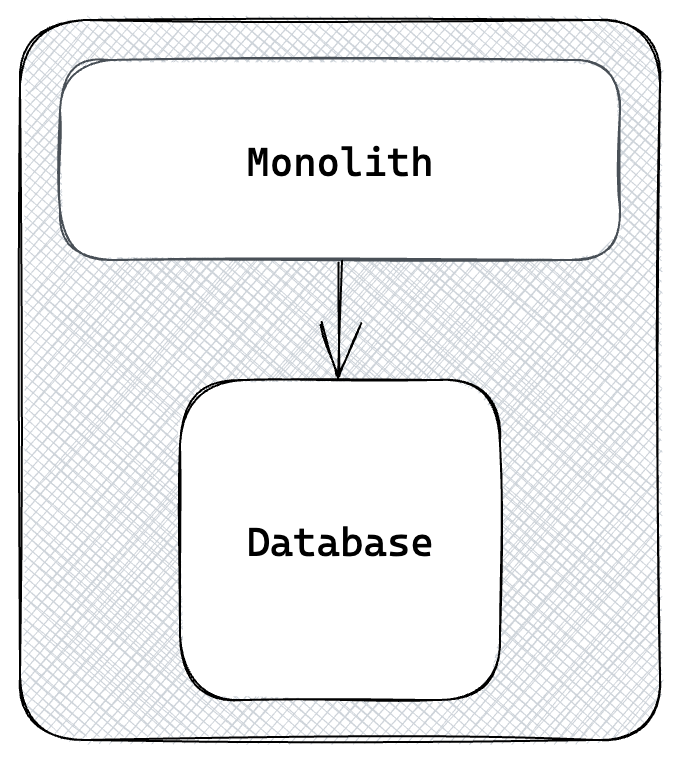
\includegraphics[width=0.3\linewidth]{images/background/monolith/monolith-sketch.png}
  \caption{The typical architecture of a software monolith. (Adapted from \cite[12]{book:2019:newman:background:monolith:monolith-to-microservices})}\label{fig:background:monolith:monolith-sketch}
\end{figure}
\fi

\bigskip

\noindent With a monolith, applying drastic changes to the complete codebase is easier. Modern \acp{IDE} support refactoring properties, for example, over the complete project. Therefore it is relatively easy to apply changes to every layer of the application, even the database schema. All project parts can be tested directly by running the application and the related database. Moreover, the complete application can be built and deployed in one step. Furthermore, it is easy to scale, as multiple instances can be run behind a load balancer. \cite[4]{book:2018:richardson:background:bff:microservices-patterns}

\bigskip

\noindent If a monolith starts to grow in size, it is essential to have a good software architecture. The code should be put in modules that follow the rules of high cohesion and low coupling of source code. The modularization splits the code into multiple chunks, which are easier to understand, but the application is still just a single process. Modules can be developed separately, but the application has to be deployed as one unit. This approach requires the coordination of various development teams. \cite[12-13]{book:2018:richardson:background:bff:microservices-patterns} \cite[12-13]{book:2019:newman:background:monolith:monolith-to-microservices} An example of such architecture is shown in the Figure \ref{fig:background:monolith:module-monolith-sketch}.

\ifshowImages
\begin{figure}[H]
    \centering
    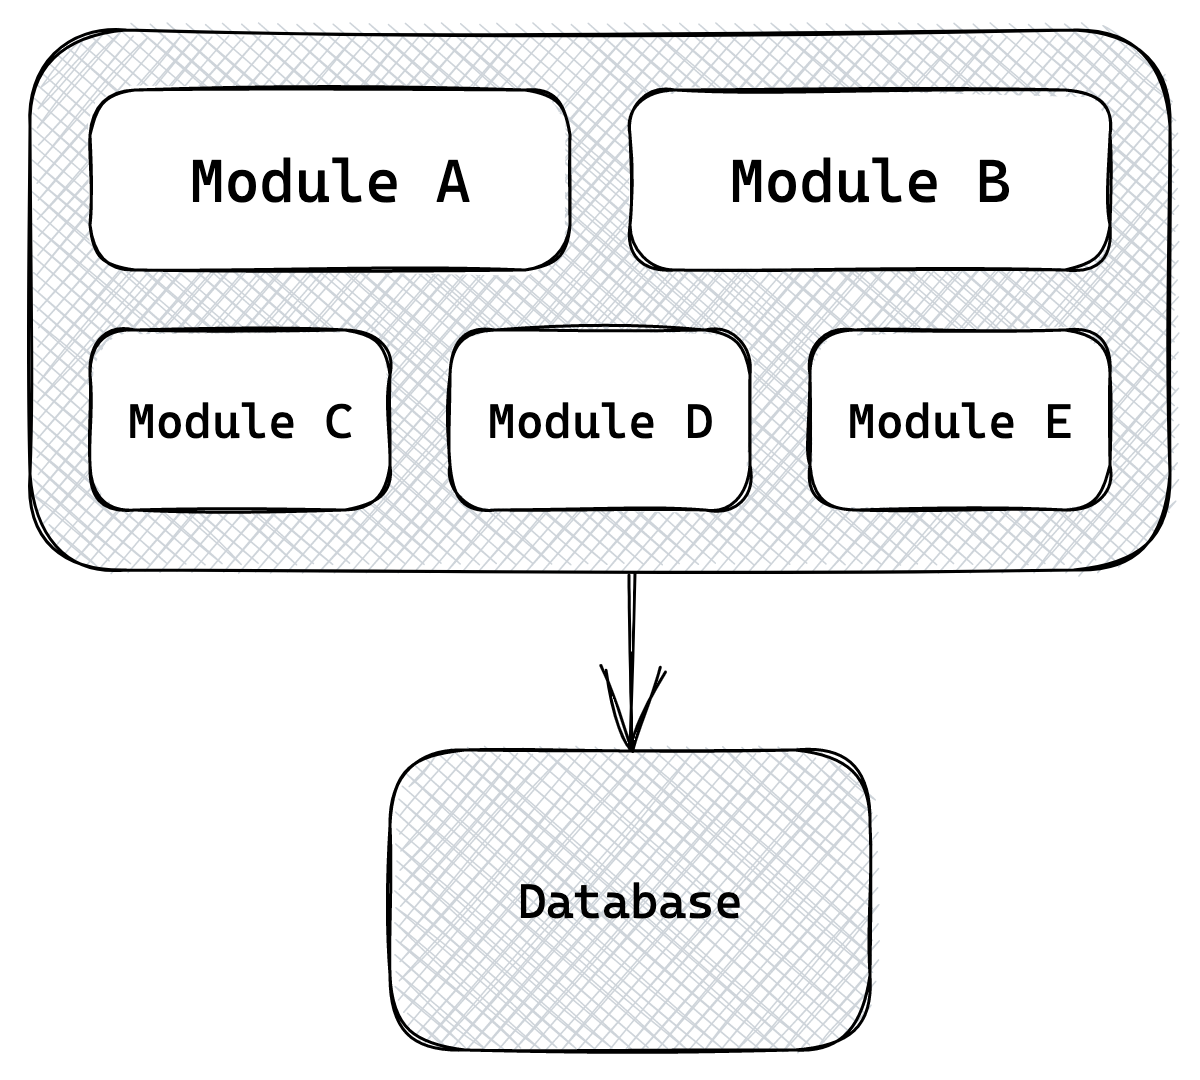
\includegraphics[width=0.4\linewidth]{images/background/monolith/modular-monolith-sketch.png}
    \caption{Structure of a modular monolith. (Adapted from \cite[13]{book:2019:newman:background:monolith:monolith-to-microservices})}\label{fig:background:monolith:module-monolith-sketch}
\end{figure}
\fi

\noindent Modular monoliths provide an excellent choice for many organizations. If there are well-defined module boundaries, parallel working is possible quite easily. However, a database cannot decompose the program logic into low-coupled modules like on the code level. \cite[12-13]{book:2019:newman:background:monolith:monolith-to-microservices}

\subsection{Disadvantages}\label{subsection:background:software-monolith:disadvantages}

With a growing code base, monolithic architectures come with increased complexity. Each new feature adds another complexity level, leading to reduced developer performance. Due to the existing entry hurdle, developing a new feature might be a very long process. The sheer size of the source code base makes it difficult to comprehend because program comprehension is an essential factor in software maintenance. \cite{article:1995:mayrhauser:background:monoliths:program-comprehension-during-software-maintenance-and-evolution} Therefore, developers might create side effects when fixing a bug. The time for developing a new feature increases drastically, and the internal architecture can also become challenging to understand and maintain. \cite[4-6]{book:2018:richardson:background:bff:microservices-patterns}

\bigskip

\noindent Another problem is that multiple teams might work on the same chunks of code. Two different developers might need to make a change to code in a shared library. A developer could change code inside a module, which he needs more information about. The change might also not be coordinated with other software engineers, which might lead to unexpected behavior in the other developer's code. The circumstance is also known as \textit{confused lines of ownership}, which are frequent sources of errors in a software system. \cite[15]{book:2019:newman:background:monolith:monolith-to-microservices} \cite[7]{inproceedings:2011:bird:background:monoliths:dont-touch-my-code}

\bigskip

\noindent With a monolithic approach, using different technologies is no longer possible, and the technology stack is restricted for the entire lifespan of the monolith. Introducing a different programming language or a different framework is impossible and often leads to a complete rewrite of an application. \cite[6-7]{book:2018:richardson:background:bff:microservices-patterns} The problem with technology is that it always becomes deprecated and obsolete at one point. Applications based on such deprecated technology must be reimplemented with a different programming language or framework. Simply rewriting the application in another framework is not straightforward because the application's functionality must be understood.

\subsubsection{Monolithic Systems are not Legacy Systems}\label{subsection:background:software-monolith:not-legacy-systems}

Developing a monolithic application should not be synonymous with writing a legacy application, and the term legacy application should not be used for monolithic systems. \cite[15]{book:2019:newman:background:monolith:monolith-to-microservices} The monolithic architecture is a good starting point for new applications. If some domains of the applications need to be better understood and when drastic changes can happen to already implemented features. It is easier to understand the complete application and make code changes. \cite[43]{book:2019:newman:background:monolith:monolith-to-microservices}


\section{API Abstraction Layer}

Every microservice provides its functionality to consumers with APIs. But it is not advisable that clients directly communicate with microservice APIs. Microservice offer fine-grained interfaces which were made especially for the communication between microservices. Therefore, the client usually has to make multiple requests to fetch the data and aggregate them to display a view inside the application. \cite{book:2021:newman:background:bff:micro-services} This leads to many requests, which is also known as over-requesting, which has a negative impact on the user experience. \cite{book:2018:richardson:background:bff:microservices-patterns}

% TODO: Progressive enhancement missing

Another problem could be that a cluster of microservices uses another form of communication. For example an asynchronous message-bus or another protocol like GRPC. Clients usually communicate using synchronous communication, where microservices might use asynchronous communication. Without an adapter in between, the communication will not work properly. Even if the communication is possible, the client needs to know many internal details about the cluster of microservices like the IP-address. It is not clear, which microservice offers the data that is needed for the client. Changing the API of a microservice would have a ripple effect on the requests on the frontends, because they would have to be changed in many places. \cite{book:2018:richardson:background:bff:microservices-patterns}

To solve this problem the clients communicate with an API gateway or a more client centric backend-for-frontend service. API gateways present an abstraction of a microservice APIs. It is the entry point to the system that is composed of multiple microservices. \cite{book:2020:siriwardena:background:bff:microservice-security-in-action}

The main task of a gateway is to forward tasks to the correct microservice and compose API for loading the needed data in one request. The even might implement functionalities like authorization and authentication or transform the protocol. Like transforming HTTP to GRPC. With API gateways it is also easier to split a microservice into two service, without a ripple effect to change all clients that consume that microservice as well. \cite{book:2018:richardson:background:bff:microservices-patterns}

But the problem with API gateways is the ownership. Multiple teams will add their functionality to the gateway and might come into conflict. The APIs are often not suited for the needs of clients and it has to be avoided that client logic is developed into the API gateway. Another pattern to bypass the problems with API gateways is the backend-for-frontend pattern. \cite{book:2018:richardson:background:bff:microservices-patterns}

With this approach each client application has its own API gateway, which is called backend-for-frontend service. This service is specially adapted for the needs of the client. \cite{book:2018:richardson:background:bff:microservices-patterns} \cite{book:2021:newman:background:bff:micro-services} This allows every team to develop their backend-for-frontend isolated and autonomous. Therefore a team can develop a complete vertical product starting from the microservice to the backend-for-frontend and finally the micro-frontend. \cite{book:2020:geers:background:micro-frontends:micro-frontends-in-action}

\subsection{Backend-for-frontend}


\section{Micro-Frontend Architecture}

Micro-frontends should bring the same advantages of microservices from the backend to the frontend. Instead of creating a large frontend monolith, a micro-frontend architecture contains many small applications. The advantage is that every micro-frontend can be developed and deployed by a separate team. \cite{book:2020:geers:background:micro-frontends:micro-frontends-in-action} The difference between frontend-monoliths and micro-frontends can be seen in figure \ref{figure:state-of-the-art:ui-monolith-micro-frontend}.

\ifshowImages
\begin{figure}[H]
\centering
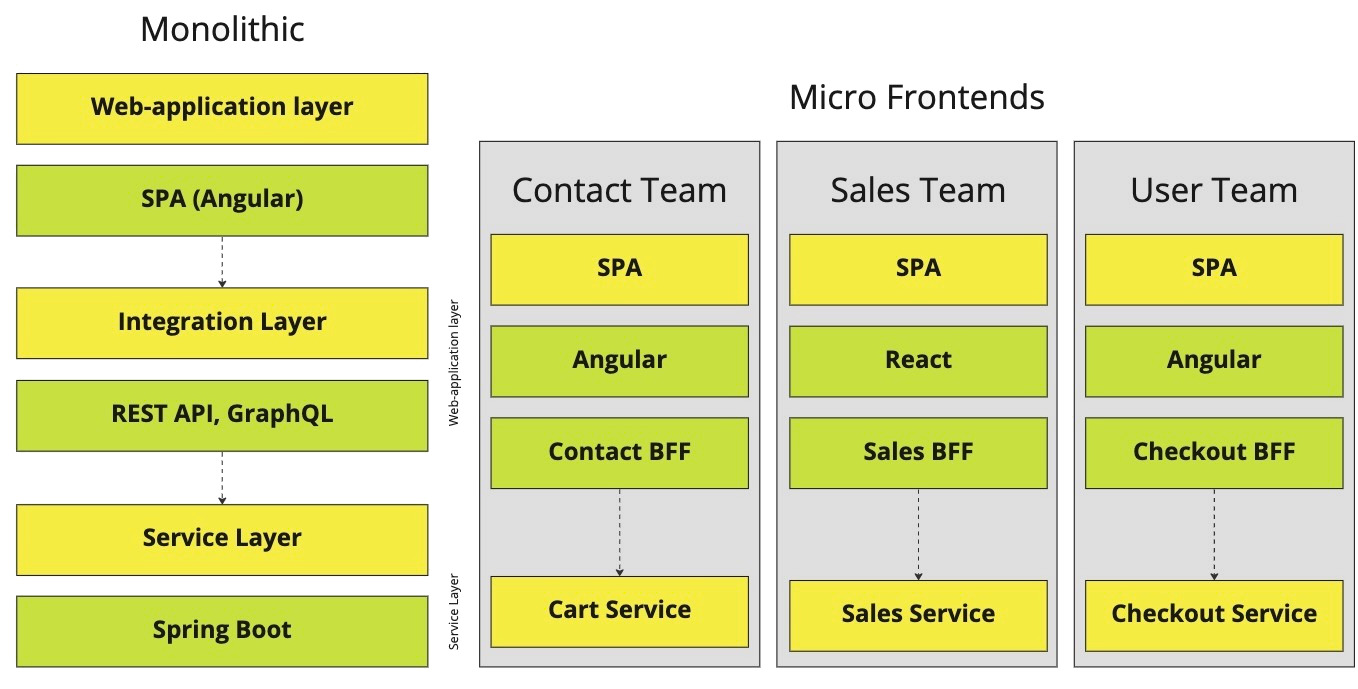
\includegraphics[width=0.8\linewidth]{images/ui-monolith-micro-frontends.jpeg}
\caption{A comparison between frontend-monoliths and micro-frontends.}\label{figure:state-of-the-art:ui-monolith-micro-frontend}
\end{figure}
\fi

Benefits gained from working with microservices on the backend are lost, when working with a monolithical frontend. With a monolithic frontend, the ability to deploy independently is lost. The entire frontend has to be deployed at once. Another problem is, that distinct operations are not really possible. If one part of the frontend is broken, there is a good chance that the entire frontend is broken. Another problem is the parallel development. The speed of development cannot be increased because it is very difficult to have multiple teams working on one frontend application. \cite{misc:2019:leitner:micro-frontends}

The term micro-frontend can be misleading, as can the term microservice. It has no meaning in terms of the size of the application. It can be a simple widget that only displays data, or a full-blown one-page application. Ideally, a micro frontend covers an area of the entire frontend application.


Micro-frontends try to apply the same principles from the microservice architecture to frontend development. Often times a microservice architecture with is developed by several teams has only one frontend application. Therefore, when adding new features a single team can be overwhelmed. Like a microservice architecture, a micro-frontend architecture focuses on developing many small frontend-applications, instead of developing a large software monolith. Each micro-frontend can be developed independently by another team. But a challenge is that the micro-frontend should appear as a single application to the user. Therefore, the different applications have to be integrated, which can be a challenge.

The term micro-frontend should not lead to false conclusions about the size of an application. The size of micro-frontends can vary. It can range from a simple login to a complex single-page application.

Building micro-frontends with the web allows different strategies of integrating the applications. Three different strategies exist to combine multiple micro-frontends into an app-shell. The client-side integration, the server-side integration and the combination of these two strategies and the combination of both strategies.

\subsection{Characteristics}

Micro-frontends tend to follow the same characteristics as microservices.

\subsubsection{Autonomous}

Technically a micro-frontend is a completely independent and runnable application. The integration of the micro-frontends happens only through the frontend. The different micro-frontends are composed withing an app-shell. The application shell is a separate application that is usually the entry-point for the user to interact with all micro-frontends. The app-shell also provides the layout of the page and defines where the micro-frontends are placed. The autonomy should not go in the direction of complete isolation. But no dependencies should emerge, which could the autonomy. \cite{book:2020:geers:background:micro-frontends:micro-frontends-in-action}

\subsubsection{Technology Agnostic}

Just as microservices architectures, micro-frontend architectures can be technology agnostic. The current frontend development landscape offers a lot of JavaScript frameworks to choose from. The advantage of an application that consists of small independent building blocks is that parts can be rewritten with another technology more easily. \cite{book:2020:geers:background:micro-frontends:micro-frontends-in-action} But using different technologies for different micro-frontends can lead to problems with the chosen form of integration and communication. The communication should be technology agnostic as well and should use browser native tools like Broadcast API.

Another problem that could arise is the bundle size of modern JavaScript frameworks. If two frameworks like React and Angular are fetched, the total bundle size can be very large and a strain for network connections. Loading an running multiple micro-frontends is also resource intensive. Due bypass this problem and offer a standardized API, micro-frontends can be developed with the help of Web Components. With this approach, no specific framework is needed to the application. \cite{book:2020:geers:background:micro-frontends:micro-frontends-in-action} 

\subsubsection{Independently Depoyable}

The autonomy of micro-frontends offer the possibility for independent deployments. A large monolithical frontend application is more complex to deploy. There is no need to have communication and coordination over multiple teams to deploy the application. Organizational dependencies have a negative impact on the time-to-market, because development teams would have to wait for the release of another team. \cite{book:2020:geers:background:micro-frontends:micro-frontends-in-action} 

\subsubsection{Small and Easy to Maintain}

Because micro-frontends only cover a small domain of an application, the source code is smaller and easier to understand. A smaller codebase is especially helpful for understanding the inner workings of software. 
Due to the easier understanding of the domain, the application can be easier rewritten with a state of the art technology, if the old one becomes deprecated. \cite{book:2020:geers:background:micro-frontends:micro-frontends-in-action}

\subsubsection{Resilience}

Micro-frontends offer the possibility to build an application by composing multiple independent applications into a fully fledged application. Depending on the integration strategy micro-frontends are usually combined at runtime. But the network, especially for mobile devices is not always without failures. A micro-frontend architecture provide better failure isolation. One micro-frontend crashing does not have an effect on the other micro-frontends inside the application. Some parts of the application might not work, but other parts of the application are still useable. The app-shell can react to a failure and tell users that the application is not working as expected and will be available back soon. \cite{article:2021:perltonen:background:micro-frontends:motivations-benefits-and-issues}

\subsection{Downsides of Micro-frontend architecture}

Due to the many advantages of micro-frontends there are also a downsides using this architectural approach. The independent development comes with the disadvantage of having redundancies. Each micro-frontend needs a separate build-process and also a continuous integration pipeline. And if the backend-for-frontend approach is, every micro-frontend needs it own backend-for-frontend service. It might happen that a lot of code is duplicated. when implementing this pattern. If multiple teams use the same code and a bug is found, the wrong behavior can't be fixed in a central place. Therefore, it is important to share knowledge between the teams to avoid running in the same bad situations over and over again. But this should not lead to inter-team dependencies between the different teams.
\cite{book:2020:geers:background:micro-frontends:micro-frontends-in-action} 


\subsection{Integration strategies}\label{subsection:background:micro-frontend-architecture:integration-strategies}

Micro-frontends can be integrated with different strategies. The integration strategy depends on the requirements of the system. They can be composed using a client-side integration strategy, a server-side strategy, or a combination of both.

\subsubsection{Server-Side Integration}\label{subsubsection:background:micro-frontend-architecture:integration-strategies:server-side-integration}

A Service between the client and the backend usually does server-side composition. \cite[60]{book:2020:geers:background:micro-frontends:micro-frontends-in-action} The server responds with references to micro-frontends that should be included and their required assets. The service in the middle intercepts that response and replaces the references to the micro-frontends with the actual content before the response is sent to the browser. The micro-frontends are included in their position and later appear in the HTML. An example of a server-side include can be seen in listing \ref{code:background:micro-frontends:server-side-include}. The other micro-frontends are referenced with URLs. \cite[61-63]{book:2020:geers:background:micro-frontends:micro-frontends-in-action}

\ifshowListings
\begin{listing}[H]
    \begin{minted}{html}
<html>
  <body>
    <!--#include virtual="/erp/dashboard" -->
  </body>
</html>
    \end{minted}
    \caption{An example server-side include.}\label{code:background:micro-frontends:server-side-include}
\end{listing}
\fi

\bigskip

\noindent One advantage of server-side integration is the fast first-load performance, which is the principle of progressive enhancement. \cite{book:2010:parker:background:micro-frontends:designing-with-progressive-enhancement} The browser fetches the HTML and renders it. It does not have to assemble parts of a page, like with client-side integration. The computation is only done on the server, which reduces the strain on the user's device. \cite{book:2020:geers:background:micro-frontends:micro-frontends-in-action} However, assets like stylesheets and images must still be fetched from the server. Server Side Integration is helpful if the application's primary concern is presenting static content to the end user and instant reaction to the users' inputs is unnecessary.  \cite[83]{book:2020:geers:background:micro-frontends:micro-frontends-in-action}

\subsubsection{Client-Side Integration}\label{subsubsection:background:micro-frontend-architecture:integration-strategies:client-side-integration}

When the application should react promptly to user input, a client-side integration strategy is preferred. For example, when developing an online marketplace, the user should be able to add items to the cart without making a complete roundtrip to the server to see the updated value. The application should provide a seamless user experience, as the end user just uses one application. Modern Frameworks like Angular and React offer the development of Single Page Applications, which provide reactive, client-side rendered applications. The HTML Markup is produced on the client instead of the server. \cite{book:2020:geers:background:micro-frontends:micro-frontends-in-action}

\bigskip

\noindent Client-side integration can be achieved through different approaches. The most straightforward approach combines the micro-frontends by linking the different applications with Hyperlinks. Each micro-frontend is deployed and accessible via a different URL, and the different micro-frontend applications are then linked with Hyperlinks. As the approach implies, switching to another micro-frontend requires a complete page reload and a roundtrip to the server. However, the integration with Hyperlinks breaks the SPA approach. This strategy makes it necessary that every micro-frontend is accessible via its URL and that it can be served as a standalone application.

\bigskip

\noindent Another client-side approach is to combine micro-frontend with iFrames or Web-Components. Integrating micro-frontends with this approach enables the page to be a SPA still. The client can navigate multiple micro-frontends without noticing, and no page reloads are needed. An iFrame is an isolated area with its own browser context \cite[35]{book:2020:geers:background:micro-frontends:micro-frontends-in-action}, Web Components are self-created HTML elements that are embedded into the DOM of the browser \cite[103]{book:2019:farrell:background:micro-frontends:web-components-in-action}. Integrating applications with the client-side strategy using Module Federation is explained in more detail in section \ref{subsubsection:background:micro-frontend:module-federation:101}.


\subsection{Communication between Micro frontends}

Micro-frontends should not depend on each other. But sometimes it is necessary have communication. For example if a user adds an item to the shopping-cart. The product micro-frontend has to inform the shopping-cart micro-frontend with the item that was added. The reduce the coupling between applications and development teams it is recommended to keep the communication at a minimum.

\subsection{Generic APIs vs Consumer Driven APIs}\label{subsection:background:micro-frontend:generic-vs-consumer-driven-apis}

The big decision in micro-frontend \ac{API} development is to use either generic or consumer-oriented \acp{API}. The difference is that generic \acp{API} emphasize reusability, while consumer-oriented \acp{API} tailor the \acp{API} to the customer.

\subsubsection{Generic \acp{API}}\label{subsubsection:background:micro-frontend:generic-vs-consumer-driven-apis:generic-apis}

Generic \acp{API} refer to \acp{API} that are very general and can be used by different clients. However, this type of \ac{API} has two significant drawbacks. Over-fetching describes the problem of getting more data than is needed, and Over-requesting describes the problem of needing multiple requests to get the data for a use case. Both problems are discussed in more detail in the following paragraphs. \cite{misc:2019:leitner:background:micro-frontends:backend-for-frontends}

\paragraph{Over-Fetching}\label{paragraph:background:micro-frontend:generic-vs-consumer-driven-apis:generic-apis:over-fetching}


For example, a contact service provides a contact model that includes \texttt{customerNumber}, \texttt{firstName}, \texttt{secondName}, \texttt{uidNumber}, and the user's address, as seen in the listing \ref{code:background:micro-frontends:over-fetching}. However, one application requirement is to display only a contact's first and last name inside the header. Only two fields of the model are used, and the rest are unnecessarily queried. \cite{misc:2019:leitner:background:micro-frontends:backend-for-frontends}

\ifshowListings
\begin{listing}[H]
    \begin{minted}{typescript}
interface ContactModel {
  id: string;
  customerNumber: string;
  firstName: string;
  secondName: string;
  uidNumber: string;

  Address: {
    id: string;
    postalCode: string;
    location: string;
    Country: string;
  }
}
    \end{minted}
    \caption{Contact-Model that contains too many fields for the requirement.}\label{code:background:micro-frontends:over-fetching}
\end{listing}
\fi

\paragraph{Over-Requesting}\label{paragraph:background:micro-frontend:generic-vs-consumer-driven-apis:generic-apis:over-requesting}

Attempting to solve the problem of over-fetching by reducing the amount of data set that is returned leads directly to this problem. Listing \ref{code:background:micro-frontends:over-requesting} shows the problem of over-requesting. If another requirement inside the application should display the address alongside the contact, two requests have to be performed every time. Afterwards, the two data sets have to be merged, leading to high client complexity. \cite{misc:2019:leitner:background:micro-frontends:backend-for-frontends}

\ifshowListings
\begin{listing}[H]
    \begin{minted}{typescript}
interface ContactModel {
  id: string;
  customerNumber: string;
  firstName: string;
  secondName: string;
  uidNumber: string;

  address_id: string;
}
    \end{minted}
    \caption{Contact-Model model that links the address-model with an id.}\label{code:background:micro-frontends:over-requesting}
\end{listing}
\fi

\subsubsection{Consumer Driven \acp{API}}\label{subsubection:background:micro-frontend:generic-vs-consumer-driven-apis:consumer-driven-apis}

Consumer-driven \acp{API} are the opposite of generic \acp{API}. They follow the idea of providing the client with exactly the data it needs. Following the example above, the contact service would have an endpoint that returns only the first and last name as required for the request. These endpoints make communication with a client straightforward, and there is no problem of over-fetching and over-requesting. However, creating an endpoint for each request creates an unmanageable set of endpoints.  \cite{misc:2019:leitner:background:micro-frontends:backend-for-frontends} To solve the problems of Over-fetching and Over-requesting, the \ac{BFF} pattern is often used. This pattern provides each client with their own \ac{API}, which is adapted to their needs. \cite{book:2018:richardson:background:bff:microservices-patterns}

\ifshowImages
\begin{figure}[H]
    \centering
    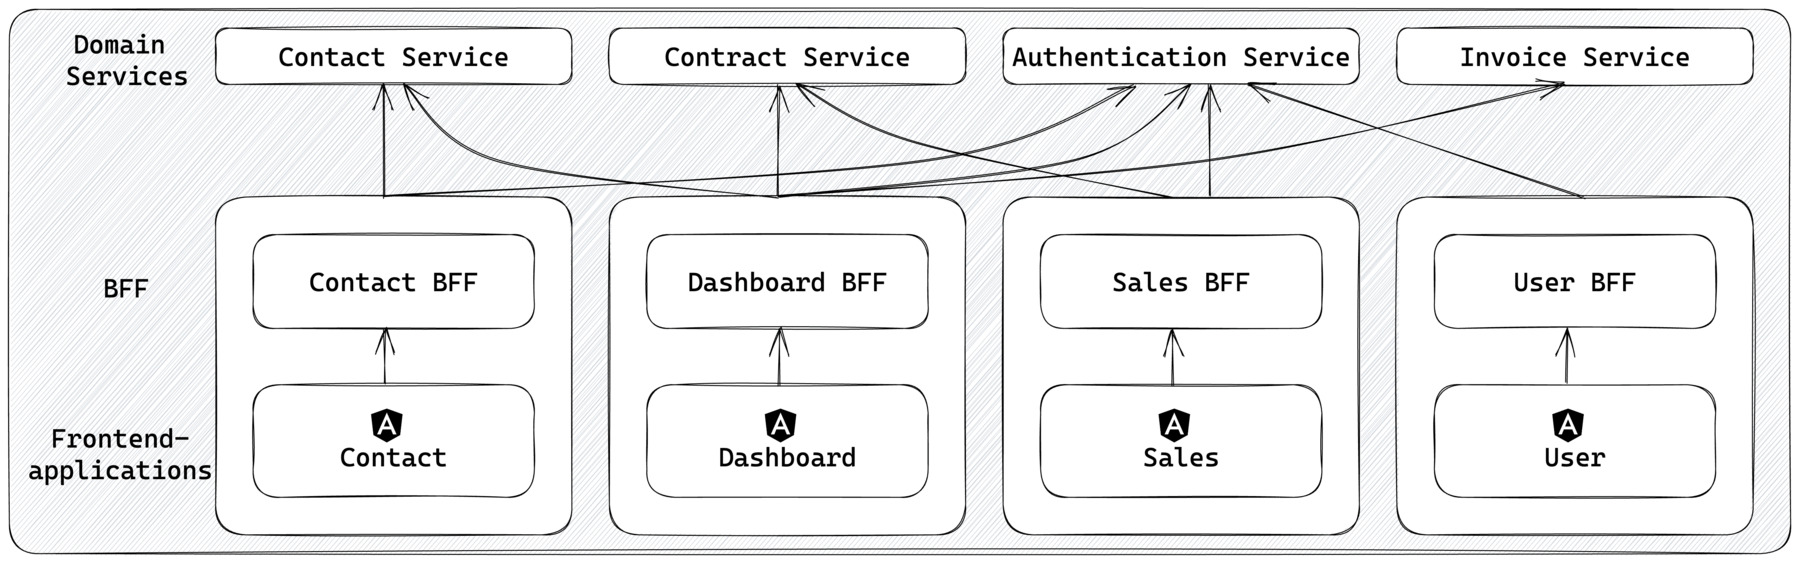
\includegraphics[width=1\linewidth]{images/background/micro-frontends/bff-architecture.jpg}
    \caption{Frontend architecture with the \ac{BFF} pattern.}\label{fig:background:micro-frontend:bff-architecture}
\end{figure}
\fi

\noindent Figure \ref{fig:background:micro-frontend:bff-architecture} shows an exemplary micro-frontend architecture using the \ac{BFF} pattern. Each frontend has a service that retrieves data only for that specific client. Because the \acp{BFF} function as a gateway to the domain services, the domain services can stay very generic and be reused by different clients. \acp{BFF} should implement only the presentation logic that puts the data into the form that the client needs, and it should avoid storing state. \cite{misc:2019:leitner:background:micro-frontends:backend-for-frontends}

\bigskip

\noindent With this architectural approach, the \ac{BFF} and the frontend form a single deployment unit. If one application changes, the other must adapt to the changes. GraphQL is a perfect technology for implementing a \ac{BFF} because it is specifically designed for implementing the presentation layer.


\section{GraphQL}\label{section:background:graphql}

GraphQL was initially developed by Facebook and refers to itself as the query language for \acp{API}. It allows the client to ask precisely for the data fields necessary. GraphQL offers the advantage that all requests can be fetched from only one endpoint. Data types provide an understandable implicit description of \ac{API} for consumers within the GraphQL schema. \cite{misc:-:background:graphql:graphql-org} The functionality of GraphQL can be compared to \ac{SQL} for databases. The client writes its queries with the desired fields from a query.

\bigskip

\noindent According to the official documentation, GraphQL is both a query language for \acp{API} and a runtime that executes those queries by using existing data. By providing a clear and comprehensive description of the data in the \ac{API}, GraphQL empowers clients to request only the data that they require, streamlining the data transfer process. This approach facilitates the evolution of \acp{API} over time and facilitates the development of powerful developer tools. The GraphQL specification is implemented in programming many languages and frameworks and has an extensive library and tool ecosystem.

\subsection{Origins and history}\label{subsection:background:graphql:origins-and-history}

GraphQL was initially developed in 2012. In 2015 the project was made open-source and available to the public. The reason behind the initial creation of GraphQL was the restricted flexibility of known \ac{API} technologies like \ac{REST}. Mobile devices needed only a subset of the fields that a \ac{REST} endpoint offered. Furthermore, the exact number of fields can change dynamically, based on the current state. The static background of \ac{REST} does not offer this behavior. Using \ac{REST}-based \acp{API} for clients that only need some fields would introduce the problem of over-fetching. Clients will be provided with information that exceeds their requirements. This approach leads to problems as mobile networks often have limited network traffic. Over-fetching puts additional strain on the user's data plan, as multiple requests have to be made. \cite{misc:2015:bryon:background:graphql:graphql-query-language}

\subsection{GraphQL Characteristics}\label{subsection:background:graphql:graphql-characteristics}

GraphQL has several design principles: \cite{misc:-:background:graphql:graphql-specification}

\begin{itemize}
  \item \textbf{Hierarchical}: Queries in GraphQL are structured hierarchically, allowing the clients to specify what data they need and in what format. This approach enables efficient data retrieval and reduces network overhead.

  \item \textbf{Product-centric}: GraphQL is designed to be product-centric rather than data-centric. That means that developers can create \acp{API} that match the needs of specific products or features rather than being constrained by the limitations of a pre-defined data schema.

  \item \textbf{Strong typing}: GraphQL is strongly-typed, meaning the data types are defined explicitly in the schema. The typing provides clarity and reduces ambiguity in the \ac{API} design while also enabling powerful tools for type checking and code generation.

  \item \textbf{Client-specified queries}: In GraphQL, the client specifies the structure of the query rather than the server. This approach allows clients to retrieve only the necessary data, reducing network overhead and enabling faster, more responsive applications.

  \item \textbf{Introspective}: GraphQL provides a built-in introspection system that enables clients to query the schema, allowing for powerful self-documentation and tooling capabilities.
\end{itemize}

\subsection{Advantages}\label{subsection:background:graphql:graphql-advantages}

GraphQL helps to reduce the network traffic between the clients and the service they query. Research indicates that the dynamic approach to fetching data can reduce the number of fields to be fetched and, therefore, the bytes sent back and forth to the GraphQL server. \cite{inprocessdings:2019:background:graphql:migration-to-graphql}

\bigskip

\noindent Because the client specifies the required fields that should be fetched, the complexity on the server can be reduced. The backend service does not need to implement many endpoints, that are only used by a small subset of clients. The \ac{API} can implement a single endpoint that all clients can query. \cite{book:2018:richardson:background:bff:microservices-patterns}

\bigskip

\noindent The characteristic that GraphQL can query its schema allows service discovery potential. Introspection allows GraphQL tools like GraphQL Voyager\footnote{\url{https://ivangoncharov.github.io/graphql-voyager/}} to visualize the schema in an \ac{UML} class diagram style. Other tools like GraphiQL\footnote{\url{https://github.com/graphql/graphiql}} can be used to analyze the schema and run queries. The functionality of such tools is explained in more detail in Section \ref{subsection:background:graphql:apollo-server-client}. \ac{REST} provides the same functionality to some degree, but additional tooling is needed because \ac{REST} cannot generate specification files.

\subsection{Disadvantages}\label{subsection:background:graphql:graphql-disadvantages}

\noindent The advantage that GraphQL reduces complexity on the server is a disadvantage for the client-side application. It leads to higher complexity when consuming GraphQL services compared to \ac{REST}. With \ac{REST}, only an endpoint has to be queried, whereas, with GraphQL, the requested data has to be specified at the field level. However, the introspection abilities of GraphQL allow consumers to understand better the query and data structure, which mitigates the disadvantage. A study \cite{inproceedings:2020:brito:background:graphql:rest-vs-graphql} showed that the study participants found it easier to consume a GraphQL Service than a \ac{REST} Service \cite{inproceedings:2017:de-pauda:background:graphql:handling-anti-patterns}. GraphQL shifts responsibilities from the server to the client, generally done with a gateway. \ac{API} composition can transfer the responsibility from the server to the client.

\bigskip

\noindent Allowing the client to specify the structure of a query might make the potential complexity of the query not transparent to the client. The approach makes it possibile that the client may specify a query which does not complete in a reasonable time or takes up a lot of resources. \cite{book:2018:richardson:background:bff:microservices-patterns}

\subsection{Apollo Server and Apollo Client}\label{subsection:background:graphql:apollo-server-client}

GraphQL has a specification and is a query language. Developing a GraphQL server and client is up to the application developer. Facebook has created its own GraphQL implementation of the specification in \ac{JS} with GraphQL.js for the backend and Relay for the frontend. Relay is a prominent example of a GraphQL client, but it is only available for Facebook's React framework. When evaluating different GraphQL clients, Apollo Client was chosen because it supports almost every possible programming language and framework.

\bigskip

\noindent Apollo Server is an open-source implementation of the GraphQL specification, and it offers any feature that the GraphQL specification states. Moreover, it supports Apollo Sandbox\footnote{\url{https://www.apollographql.com/docs/graphos/explorer/sandbox/}} out of the box. \cite{misc:-:background:graphql:apollo-server-introduction} Apollo Sandbox helps local development. Apollo Sandbox loads the GraphQL Schema from the server with the help of the Introspection Query. \cite{misc:-:background:graphql:apollo-sandbox} Such a development environment enables executing queries and mutations directly inside the browser.

\bigskip

\noindent Apollo Client is a community-driven project with npm packages for almost all frontend development environments like Angular, React, and Vue.js. The library fetches, caches, and manages the data of the application. The package for Angular is designed with Angular patterns in mind to integrate perfectly with the framework. Apollo Client offers the possibility to cache already made requests. \cite{misc:-:background:graphql:apollo-angular-client-overview} \cite{misc:-:background:graphql:apollo-client-overview} Caching is especially important as it can reduce the number of roundtrips to the server. The inner workings of the cache to prove or disprove the first hypothesis are explained in the following sections.

\subsubsection{How does the in-memory cache work?}\label{subsubsection:background:graphql:apollo-server-client:in-memory-cache-working}

This section describes how the caching mechanism of the Apollo Client works. The structure of the cache is a local, normalized, in-memory cache. All GraphQL requests made with Apollo Client are cached inside the browser's memory by default. The cache enables Apollo Client to respond almost immediately to queries for already-cached data without sending a network request. This mechanism is needed to reduce round-trips to the server in subsequent requests of the same query because the requested data can be served from the cache. \cite{misc:-:background:graphql:apollo-client-cache-overview} Caching mechanisms generally reduce the server's load but introduce issues with cache management.

\bigskip

\noindent \textbf{Apollo Client} includes a caching interface called \texttt{ApolloCache} and a proprietary implementation named \texttt{InMemoryCache}. Several Open-Source alternatives implement the \texttt{ApolloCache} interface, but Apollo's implementation is well-supported and receives regular updates.

\bigskip

\noindent Figure~\ref{fig:background:graphql:user-query-first-time} shows an exemplary query to fetch a user with its unique id. First, the Apollo Client checks whether the user with the given id is already stored inside the cache. If the query with that id has yet to be executed, a network query to fetch the user must be made. The result from the GraphQL Server is stored inside the cache and returned to the application. Four steps must be made to render data on the screen. \cite{misc:-:background:graphql:apollo-client-cache-overview}

\ifshowImages
\begin{figure}[H]
  \centering
  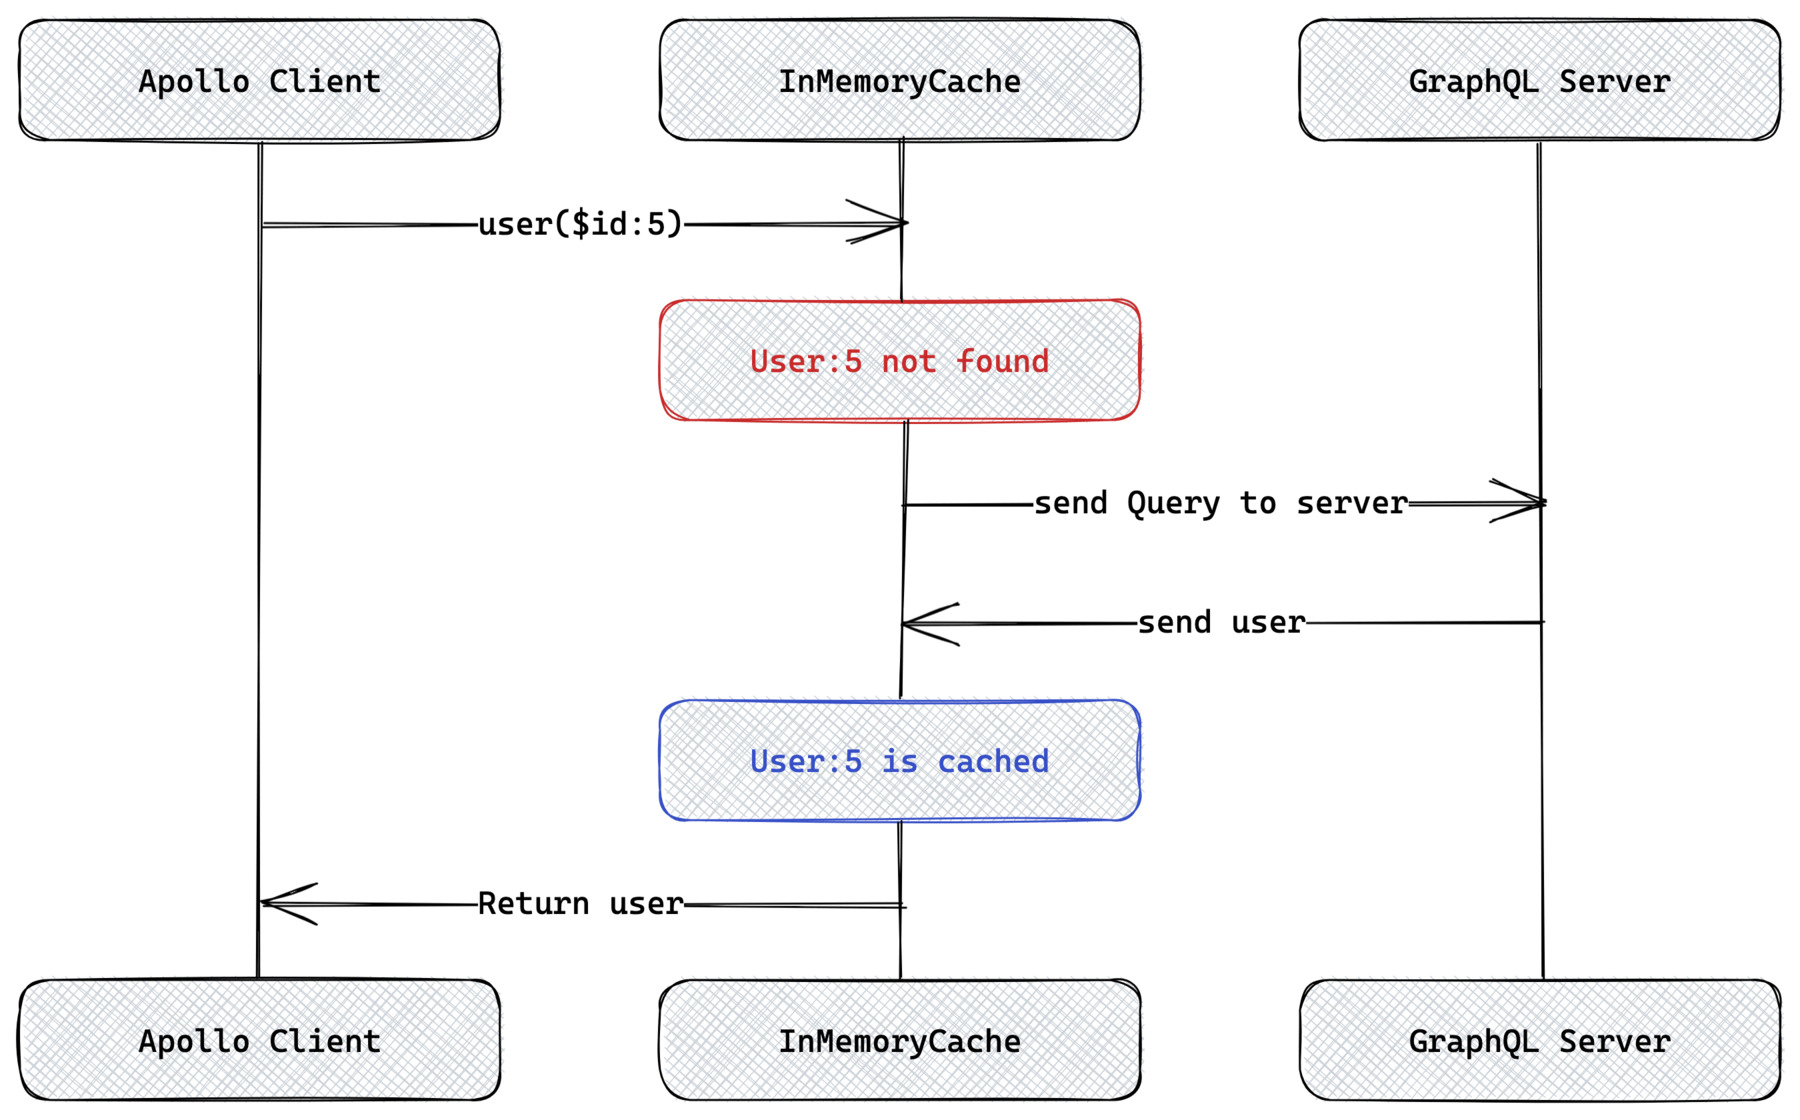
\includegraphics[width=0.6\linewidth]{images/background/graphql/apollo/apollo-client-basic-cache.jpg}
  \caption{The execution of a GraphQL query that is not stored in the cache. (Adapted from \cite{misc:-:background:graphql:apollo-client-cache-overview})}\label{fig:background:graphql:user-query-first-time}
\end{figure}
\fi

\noindent If a request with the same user id is made again, the flow of execution looks like in Figure \ref{fig:background:graphql:user-query-second-time}. As seen in the figure, no network request has to be made to the GraphQL \ac{API}, because everything is served from the Apollo Cache alone. Compared to the four steps in Figure \ref{fig:background:graphql:user-query-first-time}, only two steps need to be done here. \cite{misc:-:background:graphql:apollo-client-cache-overview}

\ifshowImages
\begin{figure}[H]
  \centering
  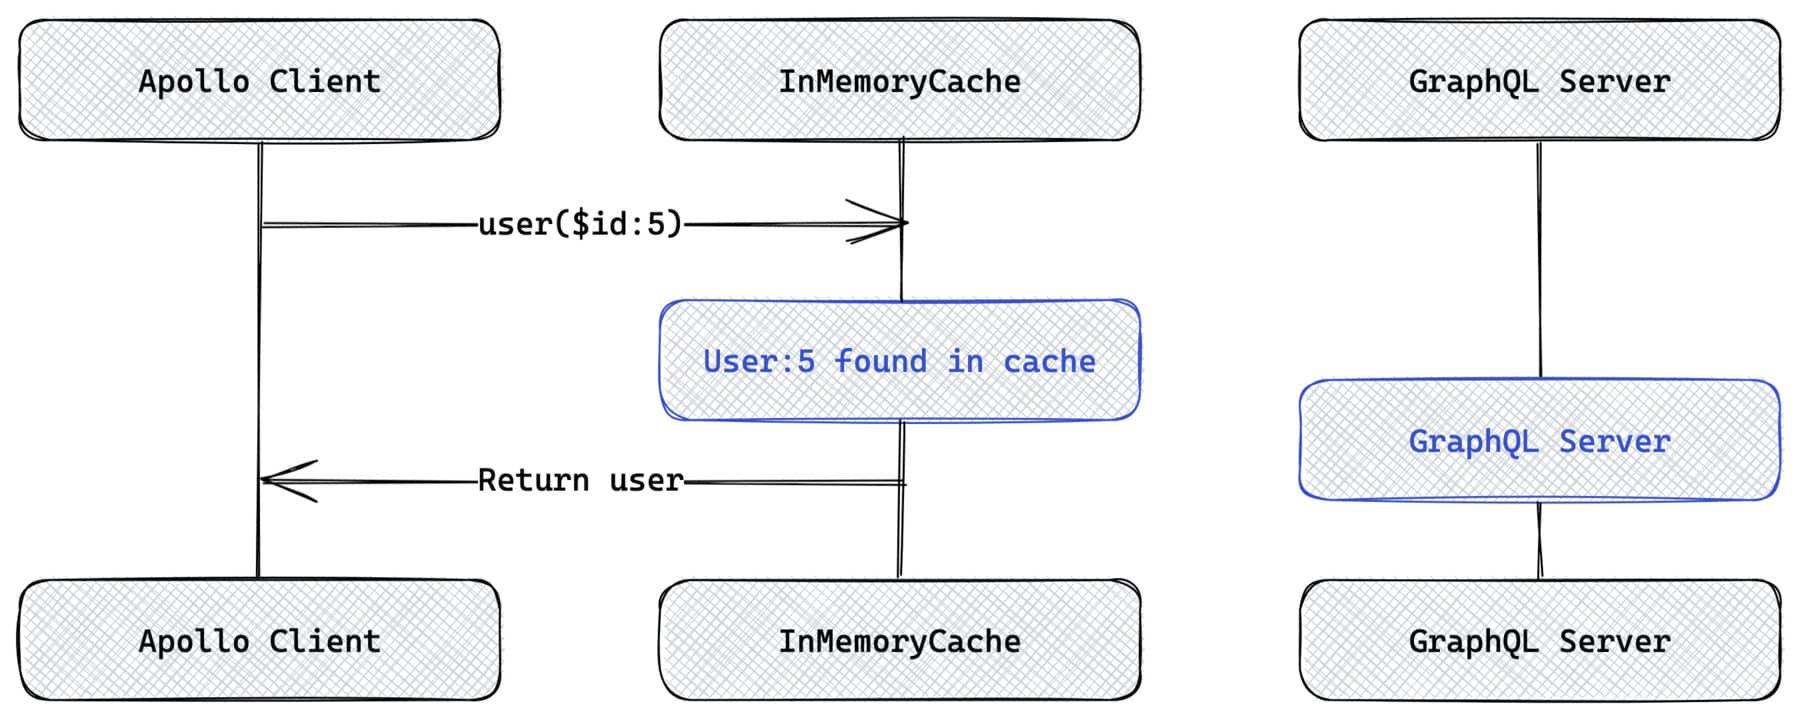
\includegraphics[width=0.7\linewidth]{images/background/graphql/apollo/apollo-client-basic-cache-warm.jpg}
  \caption{Execute the same query, which reduces the necessary steps. (Adapted from \cite{misc:-:background:graphql:apollo-client-cache-overview})}\label{fig:background:graphql:user-query-second-time}
\end{figure}
\fi

\subsubsection{Data normalization}\label{subsubsection:background:graphql:apollo-server-client:data-normalization}

Whenever the Apollo Client receives the response data of a query, it does the following. To correctly understand cache updates, it is essential to the structure of the cache before. The \texttt{InMemoryCache} is a simple normalized \ac{JS} object. The Apollo Client stores the data as a flat lookup table of objects referencing each other. An empty cache is just an empty object. These objects correspond to the objects that are returned by GraphQL queries. A single cache object might include fields fetched by multiple queries, allowing multiple queries to fetch different fields for the same object. \cite{misc:-:background:graphql:apollo-client-cache-overview} The following paragraphs describe the steps from a GraphQL query to the objects inside the cache.

\paragraph{1. Identify objects}\label{paragraph:background:graphql:apollo-server-client:data-normalization:identify-objects}

The cache identifies all distinct objects included in the query response. For example, take the query from Listing \ref{code:background:graphql:query-user-cache}, which returns the \texttt{id}, \texttt{username}, and \texttt{email} of every user.

\ifshowListings
\begin{listing}[H]
  \begin{minted}{typescript}
query {
  users {
    id
    username
    email
  }
}
  \end{minted}
  \caption{GraphQL query that fetches the id, username, and email of every user.}\label{code:background:graphql:query-user-cache}
\end{listing}
\fi

\noindent The server responds with the following response seen in Listing \ref{code:background:graphql:query-user-response-result}. The \texttt{\_\_typename} property is automatically appended to the query by the Apollo Client to identify the object.

\ifshowListings
\begin{listing}[H]
  \begin{minted}{typescript}
{
  users: [
    {
      __typename: 'User',
      id: '36bad921-8fcf-4f33-9f29-0d3cd70205c8',
      username: 'Florian',
      email: 'florian@test.io'
    },
    {
      __typename: 'User',
      id: 'a2096556-9a4e-4994-9de8-86c9e85ed6a1',
      username: 'Lisa',
      email: 'lisa@test.io'
    }
  ]
}
  \end{minted}
  \caption{The result of the GraphQL query from Listing \ref{code:background:graphql:query-user-cache}.}\label{code:background:graphql:query-user-response-result}
\end{listing}
\fi

The caching mechanism identifies the following objects to be cached.

\begin{itemize}
  \item A \texttt{User} with id \texttt{36bad921-8fcf-4f33-9f29-0d3cd70205c8}
  \item A \texttt{User} with id \texttt{a2096556-9a4e-4994-9de8-86c9e85ed6a1}
\end{itemize}

\paragraph{2. Generate cache IDs}\label{paragraph:background:graphql:apollo-server-client:data-normalization:generate-cache-ids}

After identifying all objects, the cache generates a cache ID for each object. A cache ID uniquely identifies a particular object while it is in the \texttt{InMemoryCache}.

\noindent So, the cache IDs for the objects from the previous section are:

\begin{itemize}
    \item \texttt{User:36bad921-8fcf-4f33-9f29-0d3cd70205c8}
    \item \texttt{User:a2096556-9a4e-4994-9de8-86c9e85ed6a1}
\end{itemize}

\noindent By default, an object's cache ID is concatenated with the object's \texttt{\_\_typename} and \texttt{id} (or \texttt{\_id}) fields. If the cache cannot generate a cache ID for a particular object, that object is directly stored inside its parent object and must be referenced via the parent. Therefore the cache is not always completely flat. This behavior is shown with the query in Listing \ref{code:background:graphql:no-id-query-user-cache}. 

\ifshowListings
\begin{listing}[H]
  \begin{minted}{typescript}
query {
  allUsers {
    id
    username
    Title {
      name
    }
  }
}
  \end{minted}
  \caption{Fetch the \texttt{id}, \texttt{username} and the \texttt{name} of the title of the user, without the \texttt{id} of the title.}\label{code:background:graphql:no-id-query-user-cache}
\end{listing}
\fi

\noindent The query from the listing misses the \texttt{id} field inside the Title field. Therefore the cache stores the Title object directly inside the user object. The result inside the cache is shown in the listing
\ref{code:background:graphql:no-id-query-user-cache-representation}. 

\ifshowListings
\begin{listing}[H]
  \begin{minted}{typescript}
{
  'User:36bad921-8fcf-4f33-9f29-0d3cd70205c8': {
    __typeName: 'User',
    id: '36bad921-8fcf-4f33-9f29-0d3cd70205c8',
    username: 'Florian',
    Title: { name: 'BSc.' }
  },
  'User:a2096556-9a4e-4994-9de8-86c9e85ed6a1': {
    __typeName: 'User',
    id: 'a2096556-9a4e-4994-9de8-86c9e85ed6a1',
    username: 'Lisa',
    Title: { name: 'BSc.' }
  }
}
  \end{minted}
  \caption{The content of the cache after fetching the query from Listing \ref{code:background:graphql:no-id-query-user-cache}.}\label{code:background:graphql:no-id-query-user-cache-representation}
\end{listing}
\fi

\noindent Omitting IDs from a query should be avoided. If data of an un-normalized object has to be updated, every occurrence of the item in the cache has to be updated manually. It should be avoided that the same thing is queried, sometimes with an id and sometimes without, because Apollo Client will throw an error when trying to update the cache after such a query.

\paragraph{3. Replace object fields with references}\label{paragraph:background:graphql:apollo-server-client:data-normalization:replace-object-fields-with-references}

Next, the cache takes each field that contains an object and replaces its value with a reference to the appropriate object. Listing \ref{code:background:graphql:nested-query-user-cache} shows a query that demonstrates how the objects from a query are transformed in the \texttt{InMemoryCache} representation.

\ifshowListings
\begin{listing}[H]
  \begin{minted}{typescript}
query {
  allUsers {
    id
    username
    Title {
      id
      name
    }
  }
}
  \end{minted}
  \caption{A GraphQL query to fetch all users.}\label{code:background:graphql:nested-query-user-cache}
\end{listing}
\fi

Listing \ref{code:background:graphql:nested-query-response-user-cache} shows a single result from the GraphQL server for the query from Listing \ref{code:background:graphql:nested-query-user-cache}.

\ifshowListings
\begin{listing}[H]
    \begin{minted}{typescript}
{
  __typename: 'User',
  id: '36bad921-8fcf-4f33-9f29-0d3cd70205c8',
  username: 'Florian',
  title: {
    __typename: 'Title',
    id: '2adb1120-d911-4196-ab1b-d5043cc7a00a',
    name: 'BSc.'
  }
}
    \end{minted}
    \caption{The result of the GraphQL query from Listing \ref{code:background:graphql:nested-query-user-cache}.} \label{code:background:graphql:nested-query-response-user-cache}
\end{listing}
\fi

\noindent And Listing \ref{code:background:graphql:nested-query-response-after-replacement} shows how the object is stored inside the \texttt{InMemoryCache}.

\ifshowListings
\begin{listing}[H]
  \begin{minted}{typescript}
{
  __typename: 'User',
  id: '36bad921-8fcf-4f33-9f29-0d3cd70205c8',
  username: 'Florian',
  title: { __ref: 'Title:36bad921-8fcf-4f33-9f29-0d3cd70205c8' }
}
  \end{minted}
  \caption{The structure of the cache after the user object is stored.}\label{code:background:graphql:nested-query-response-after-replacement}
\end{listing}
\fi

\noindent The \texttt{title} field now references the appropriate normalized \texttt{Title} object. If another \texttt{User} with the same \texttt{title} is stored inside the in-memory cache, that normalized \texttt{Title} object is reused. Normalization can drastically reduce data duplication inside the cache, and it also helps to make the data stay synchronous with the server.

\paragraph{4. Store normalized objects}\label{paragraph:background:graphql:apollo-server-client:data-normalization:store-normalized-objects}

The resulting objects are stored inside the cache's flat lookup table. Whenever an incoming object has the same cache ID as an existing cached object, the fields of those objects are merged. If the incoming and the existing object share existing fields, the incoming object overwrites the cached value for those fields. Fields that exist in only one object are preserved. This normalization constructs a partial copy of the graph on our client. \cite{misc:-:background:graphql:apollo-client-cache-overview}

\bigskip

\noindent Listing \ref{code:background:graphql:nested-query-user-cache-representation} shows how normalized objects are stored. Each user contains a reference to a title. Both users have the same title. Therefore the server returned duplicate data. However, the cache normalization causes the title to be only present once inside the cache. This behavior is constructive because when a cache item is updated, the entire cache object does not have to be traversed in search of the instance that has been changed. Only a single item has to be updated. The cache normalization works when the query contains either a \texttt{\_id} or \texttt{id} field.

\ifshowListings
\begin{listing}[H]
    \begin{minted}{typescript}
{
  'User:36bad921-8fcf-4f33-9f29-0d3cd70205c8': {
    __typeName: 'User',
    id: '36bad921-8fcf-4f33-9f29-0d3cd70205c8',
    username: 'Florian',
    Title: { __ref: 'Title:2adb1120-d911-4196-ab1b-d5043cc7a00a' },
  },
  'User:a2096556-9a4e-4994-9de8-86c9e85ed6a1': {
    __typeName: 'User',
    id: 'a2096556-9a4e-4994-9de8-86c9e85ed6a1',
    username: 'Lisa',
    Title: { __ref: 'Title:2adb1120-d911-4196-ab1b-d5043cc7a00a' },
  }
  'Title:2adb1120-d911-4196-ab1b-d5043cc7a00a': {
    __typeName: 'Title',
    id: '2adb1120-d911-4196-ab1b-d5043cc7a00a',
    name: 'BSc.',
  },
}
  \end{minted}
  \caption{The structure of the cache with the result from the query from Listing \ref{code:background:graphql:nested-query-user-cache}.}\label{code:background:graphql:nested-query-user-cache-representation}
\end{listing}
\fi

\subsubsection{Understanding the structure of the cache}\label{subsubsection:background:graphql:apollo-server-client:understanding-cache-structure}

Apollo Client offers development tools for the browser in the form of browser extensions. The Apollo Client Developer Tools\footnote{\url{https://chrome.google.com/webstore/detail/apollo-client-devtools/jdkknkkbebbapilgoeccciglkfbmbnfm}} can be installed for Chrome and Firefox. The extension can be found in the Chrome Web Store and the Firefox Add-ons Store. The browser extension adds a tab to the browser inspection tools. \cite{misc:-:background:graphql:apollo-developer-tools} The view of the cache contents from the Apollo Client Development Tools can be seen in Figure \ref{fig:background:graphql:apollo:apollo-dev-tools}.

\ifshowImages
  \begin{figure}[H]
    \centering
    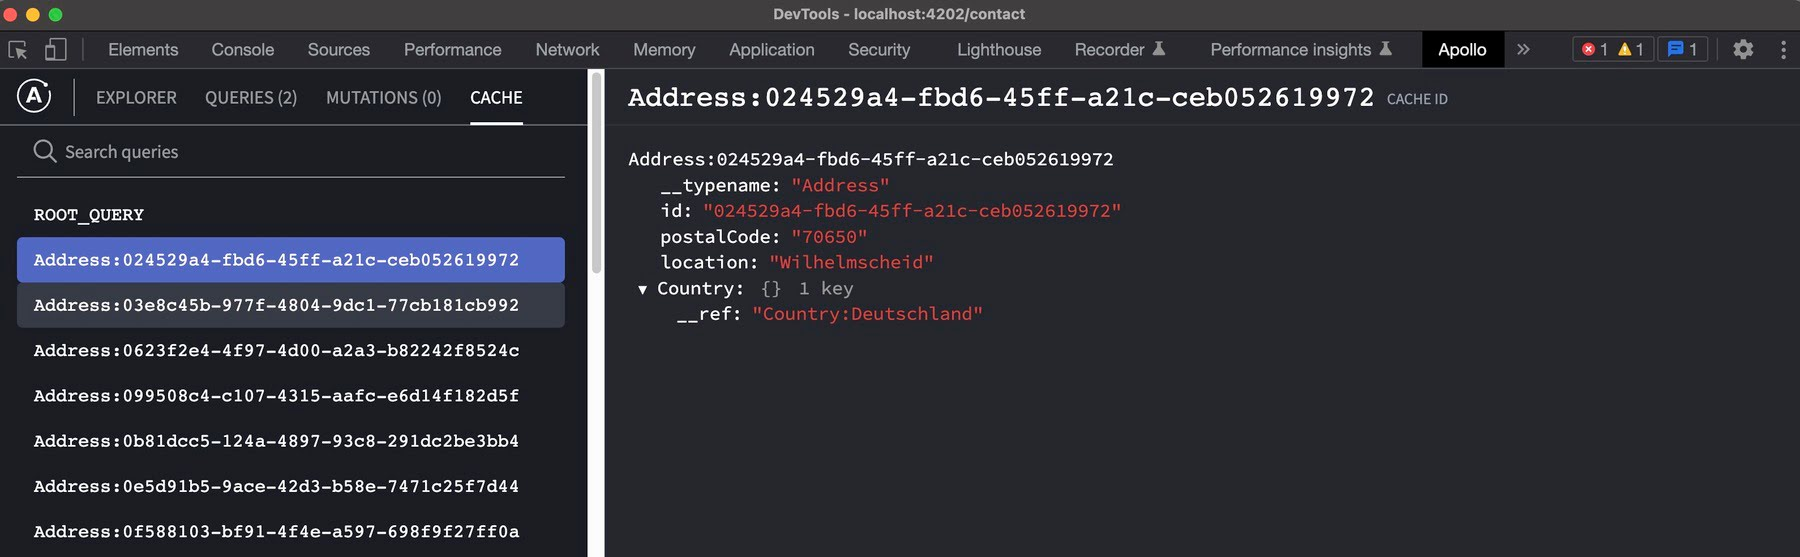
\includegraphics[width=1\linewidth]{images/background/graphql/apollo/apollo-dev-tools.jpg}
    \caption{The content of the cache inside the Apollo Client Developer Tools.}\label{fig:background:graphql:apollo:apollo-dev-tools}
  \end{figure}
\fi

\noindent The development tools offer the following four main features: \cite{misc:-:background:graphql:apollo-developer-tools}

\begin{itemize}
  \item \textbf{GraphiQL}: Send queries to the server through the web application's configured Apollo Client instance, or query the Apollo Client cache to see what data is loaded.
  \item \textbf{Watched query inspector}: View active queries, variables, cached results, and re-run individual queries.
  \item \textbf{Mutation inspector}: View active mutations and their variables, and re-run individual mutations.
  \item \textbf{Cache inspector}: Visualize the Apollo Client and search it by field name and/or value.
\end{itemize}

\noindent Another method to access the content of the cache is through the \texttt{window} object in \ac{JS}. The object can be accessed through \texttt{window.\_\_APOLLO\_CLIENT\_\_.cache.extract()} inside the browser's development tools. The result of this method invocation can be seen in Figure \ref{fig:background:graphql:apollo:apollo-cache-browser-window}.

\ifshowImages
  \begin{figure}[H]
    \centering
    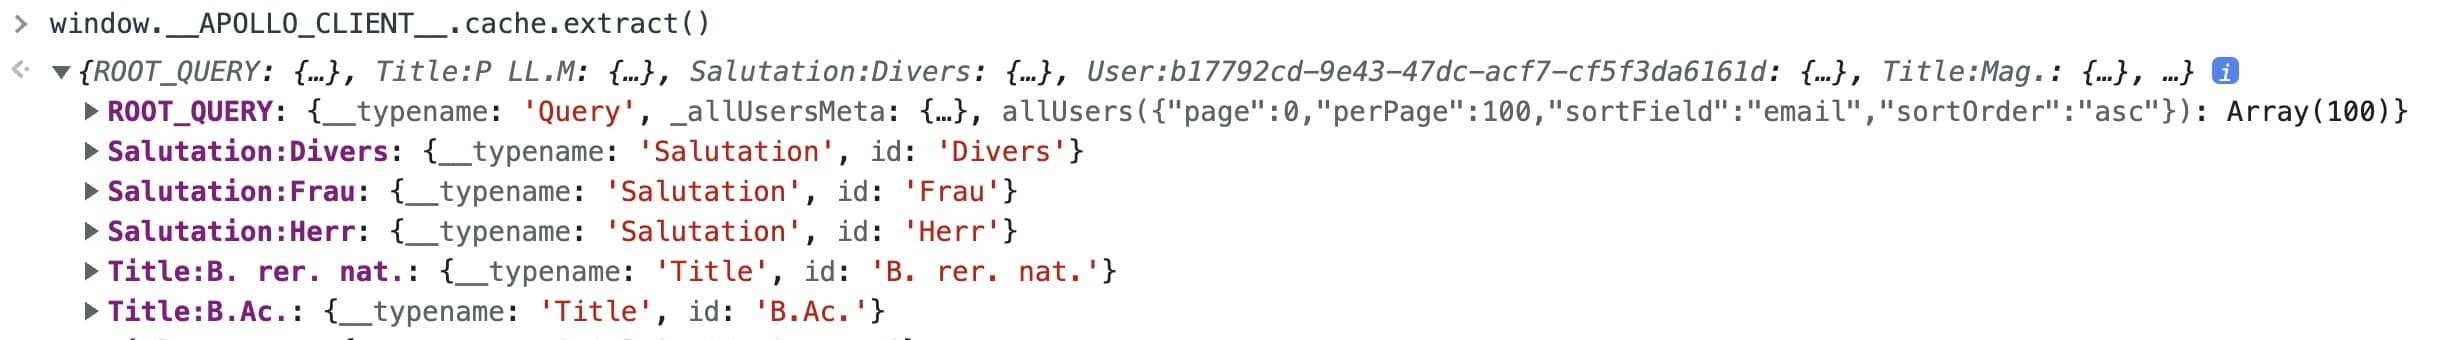
\includegraphics[width=1\linewidth]{images/background/graphql/apollo/apollo-cache-browser-window.jpg}
    \caption{View the content of the cache inside the development tools.}\label{fig:background:graphql:apollo:apollo-cache-browser-window}
  \end{figure}
\fi

\noindent With this approach, the content of the cache can be explored with the help of \ac{JS} methods inside the browser development tools.

\subsubsection{Type-Policies}\label{subsubsection:background:graphql:apollo-server-client:type-policies}

Type policies are a way to define how the client stores and manages data in the cache. The constructor of the \texttt{InMemoryCache} accepts type policies as an object. The \texttt{typePolicies} object the behavior of the cache can be customized on a type-by-type basis. Type policies are fine-grained; they allow to customize how a specific field inside the cache is read and written. A type policy contains multiple field policies that customize the behavior of the fields for that type. \cite{misc:-:background:graphql:apollo-client-cache-reading-writing}

\bigskip

\noindent A field policy for a field consists of: \cite{misc:-:background:graphql:apollo-client-cache-reading-writing}

\begin{itemize}
  \item A \texttt{read} function which is called when the field is read from the cache.
  \item A \texttt{merge} function which is called when the field is written to the cache.
  \item An array of fields, which are the key arguments that identify an object. This so-called \texttt{keyArgs} avoids storing duplicate data in the cache.
\end{itemize}

\paragraph{Read function}

Listing \ref{code:background:graphql:read-type-policy} shows the definition of a \texttt{read} function. The cache calls that function when the client queries for a user's first name. The \texttt{InMemoryCache} then returns the function's response instead of the cached value. The first parameter of the function is the current value of the field. The second parameter is an object that contains the arguments of the field and several helper functions and properties. \cite{misc:-:background:graphql:apollo-client-cache-reading-writing} The \texttt{read} function of Listing \ref{code:background:graphql:read-type-policy} returns a default value for the \texttt{firstName} of the \texttt{User} type when a value is unavailable in the cache. If a value exists in the cache, the value is returned unmodified.

\ifshowListings
\begin{listing}[H]
    \begin{minted}{typescript}
new InMemoryCache({
  typePolicies: { User: { fields: {
    firstName: {
      read(value, options) {
        return value ?? 'Unknown';
      }
    }
  }}}
});
    \end{minted}
    \caption{Provide a default value for the  \texttt{firstName} field.}\label{code:background:graphql:read-type-policy}
\end{listing}
\fi

\paragraph{Merge function}

The \texttt{merge} function for a field is called whenever the field is about to be written with an incoming value. The field's new value is set to the \texttt{merge} function's return value instead of the original value.  An everyday use case for the \texttt{merge} function is to define a field policy for a field that holds an array. By default, the existing collection is completely replaced by the incoming array. However, sometimes, both arrays should be concatenated. This pattern is used with paginated lists, where the incoming page should be merged with the existing pages. The parameters are the current value, the incoming value, and the options, just like in the \texttt{read} function. \cite{misc:-:background:graphql:apollo-client-cache-reading-writing}

\bigskip

\noindent Listing \ref{code:background:graphql:write-type-policy} shows the definition of a \texttt{merge} function. Whenever a new transaction for the bank account is fetched, the existing and the incoming transactions are merged. Initially, \texttt{existing} is undefined; therefore, \texttt{existing} is assigned a default parameter.

\ifshowListings
\begin{listing}[H]
    \begin{minted}{typescript}
new InMemoryCache({
  typePolicies: { BankAccount: { fields: {
    transaction: {
      merge(existing = [], incoming: unknown[], options) {
        return [...existing, ...incoming];
      },
    },
  }}},
});
    \end{minted}
    \caption{Merge the existing and incoming transactions in a \texttt{merge} function.}\label{code:background:graphql:write-type-policy}
\end{listing}
\fi

\subsection{Query Reduction}

This section describes the theory behind reducing queries with already existing data inside the cache. Apollo Client does not offer this behavior by default. The Github repository features a lot of feature requests that want such a feature implemented for queries. Unfortunately this did not happen. The next section describes how the theory behind reduction works.

\subsubsection{Theoretical Concept}

In large applications, it is likely that the same query is executed with different selection sets over and over again. Unless the selection set of the query is perfectly identical, Apollo Client will fetch the query from the server. Ignoring the fact that many of the queries fields are already inside the cache. An example query is shown in listing \ref{code:background:graphql:query-reduction:example-query-simple}

\ifshowListings
\begin{listing}[H]
\begin{minted}{typescript}
query {
  allUsers {
    id
    username
    Title {
      id
      name
    }
  }
  allTitles {
    id
    name
  }
}
\end{minted}
\caption{An exemplary GraphQL query that fetches all users}\label{code:background:graphql:query-reduction:example-query-simple}
\end{listing}
\fi

The first time this query is executed, a request is sent to the server. Each subsequent execution of the query with the same selection set is served from the cache and a round trip to the server is saved. Afterwards the same query is executed with a different selection set. The query is sent to the server again, even though the selection set is only slightly different. The selection set of the query is extended by the email field and is shown in listing \ref{code:background:graphql:query-reduction:example-query-extended}

\ifshowListings
\begin{listing}[H]
\begin{minted}{typescript}
query {
  allUsers {
    id
    username
    email // Additional field
    Title {
      id
      name
    }
  }
  allTitles {
    id
    name
  }
}
\end{minted}
\caption{An exemplary GraphQL query that fetches all users with an additional field}\label{code:background:graphql:query-reduction:example-query-extended}
\end{listing}
\fi

The queries are almost identical, but there is an additional field, this will result in a cache miss. The entire query will be requested from the server. This is quite unnecessary because the most part of the data is already in the cache. A better approach would be to fetch only the field which is missing inside the cache like shown in \ref{code:background:graphql:query-reduction:example-query-reduced}.

\ifshowListings
\begin{listing}[H]
\begin{minted}{typescript}
query {
  allUsers {
    id
    email
  }
}
\end{minted}
\caption{The part of the exemplary query that is necessary}\label{code:background:graphql:query-reduction:example-query-reduced}
\end{listing}
\fi

The id can't be removed from the query as it needed to merge the existing and incoming data together afterwards. Depending how many shared selections exist inside the application's queries, a lot of server resources can be saved by reducing the queries. 





\chapter{Applied Methods}\label{chapter:applied-methods}

This chapter documents how the prototype micro-frontend architecture was built step by step. It starts with building the foundation of the application and continues with building the communication between the shell and the remote application. Then, with the common caching layer and the reduction of queries, the basis for the evaluation of the hypothesis of the work was established. The final section is a comparison between the original and reduced queries.

\section{Identification of micro-frontends}\label{section:applied-methods:identification-micro-frontends}

The first step before starting to implement the micro-frontend architecture was to identify the parts of the legacy application that should be extracted into microservices and micro-frontends. The application is a large software monolith with a single database. In collaboration with the product owner, the bounded contexts of the legacy application were identified as candidates for micro-frontends and microservices. 

\bigskip

\noindent The complete legacy application can't be prototyped in the course of this master thesis, therefore the three most important bounded contexts were identified. The first bounded contexts to implement are the following:

\begin{itemize}
  \item User
  \item Sales
  \item Contact
  \item Dashboard
\end{itemize}
%% \section{GraphQL client comparison}

\section{Implementing a prototypical micro-frontend architecture}\label{section:applied-methods:prototypical-implementation}

The first step was to implement a prototypical micro-frontend application to evaluate the hypothesis. The base architecture was developed to lay the groundwork for later use in a production environment. The micro-frontends are integrated using client-side integration, more precisely, run-time integration. The integration strategy was implemented with Webpack's Module Federation, which was described in more detail in Section \ref{subsection:background:micro-frontend:module-federation}. The majority of the implementation is written in Angular. One micro-frontend was implemented in React to showcase the technology agnosticism of the caching strategy. The prototype contains an application shell that consumes the other micro-frontends. The architecture is divided into nine widgets that display only simple data and four complex single-page applications. The four \acp{SPA} are Dashboard, Contact, Sales, and User.

\bigskip

\noindent The library Nx from the company Nwrl is used for managing the micro-frontends and libraries in a single monorepo. An essential feature of Nx is the support for monorepos, which is the perfect match for managing micro-frontend applications. It offers support and tooling for almost any \ac{JS} framework and can be customized with plugins. Multiple related projects can be managed in a single workspace. Additionally, it ensures that every project uses the same version of a dependency across the workspace. Besides, Nx offers helper functions for working with Module Federation in micro-frontends. \cite{misc:-:applied-methods:intro-to-nx}

\bigskip

\noindent A rough overview of the architecture is shown in Figure \ref{fig:applied-methods:prototype-micro-frontend-architecture}. It shows a wireframe of the structure of the application. The icons inside the squares represent the \ac{JS} framework used. Each widget is a separate micro-frontend that exposes a remote module through Module Federation, which is then consumed by the Dashboard micro-frontend.

\ifshowImages
\begin{figure}[H]
  \centering
  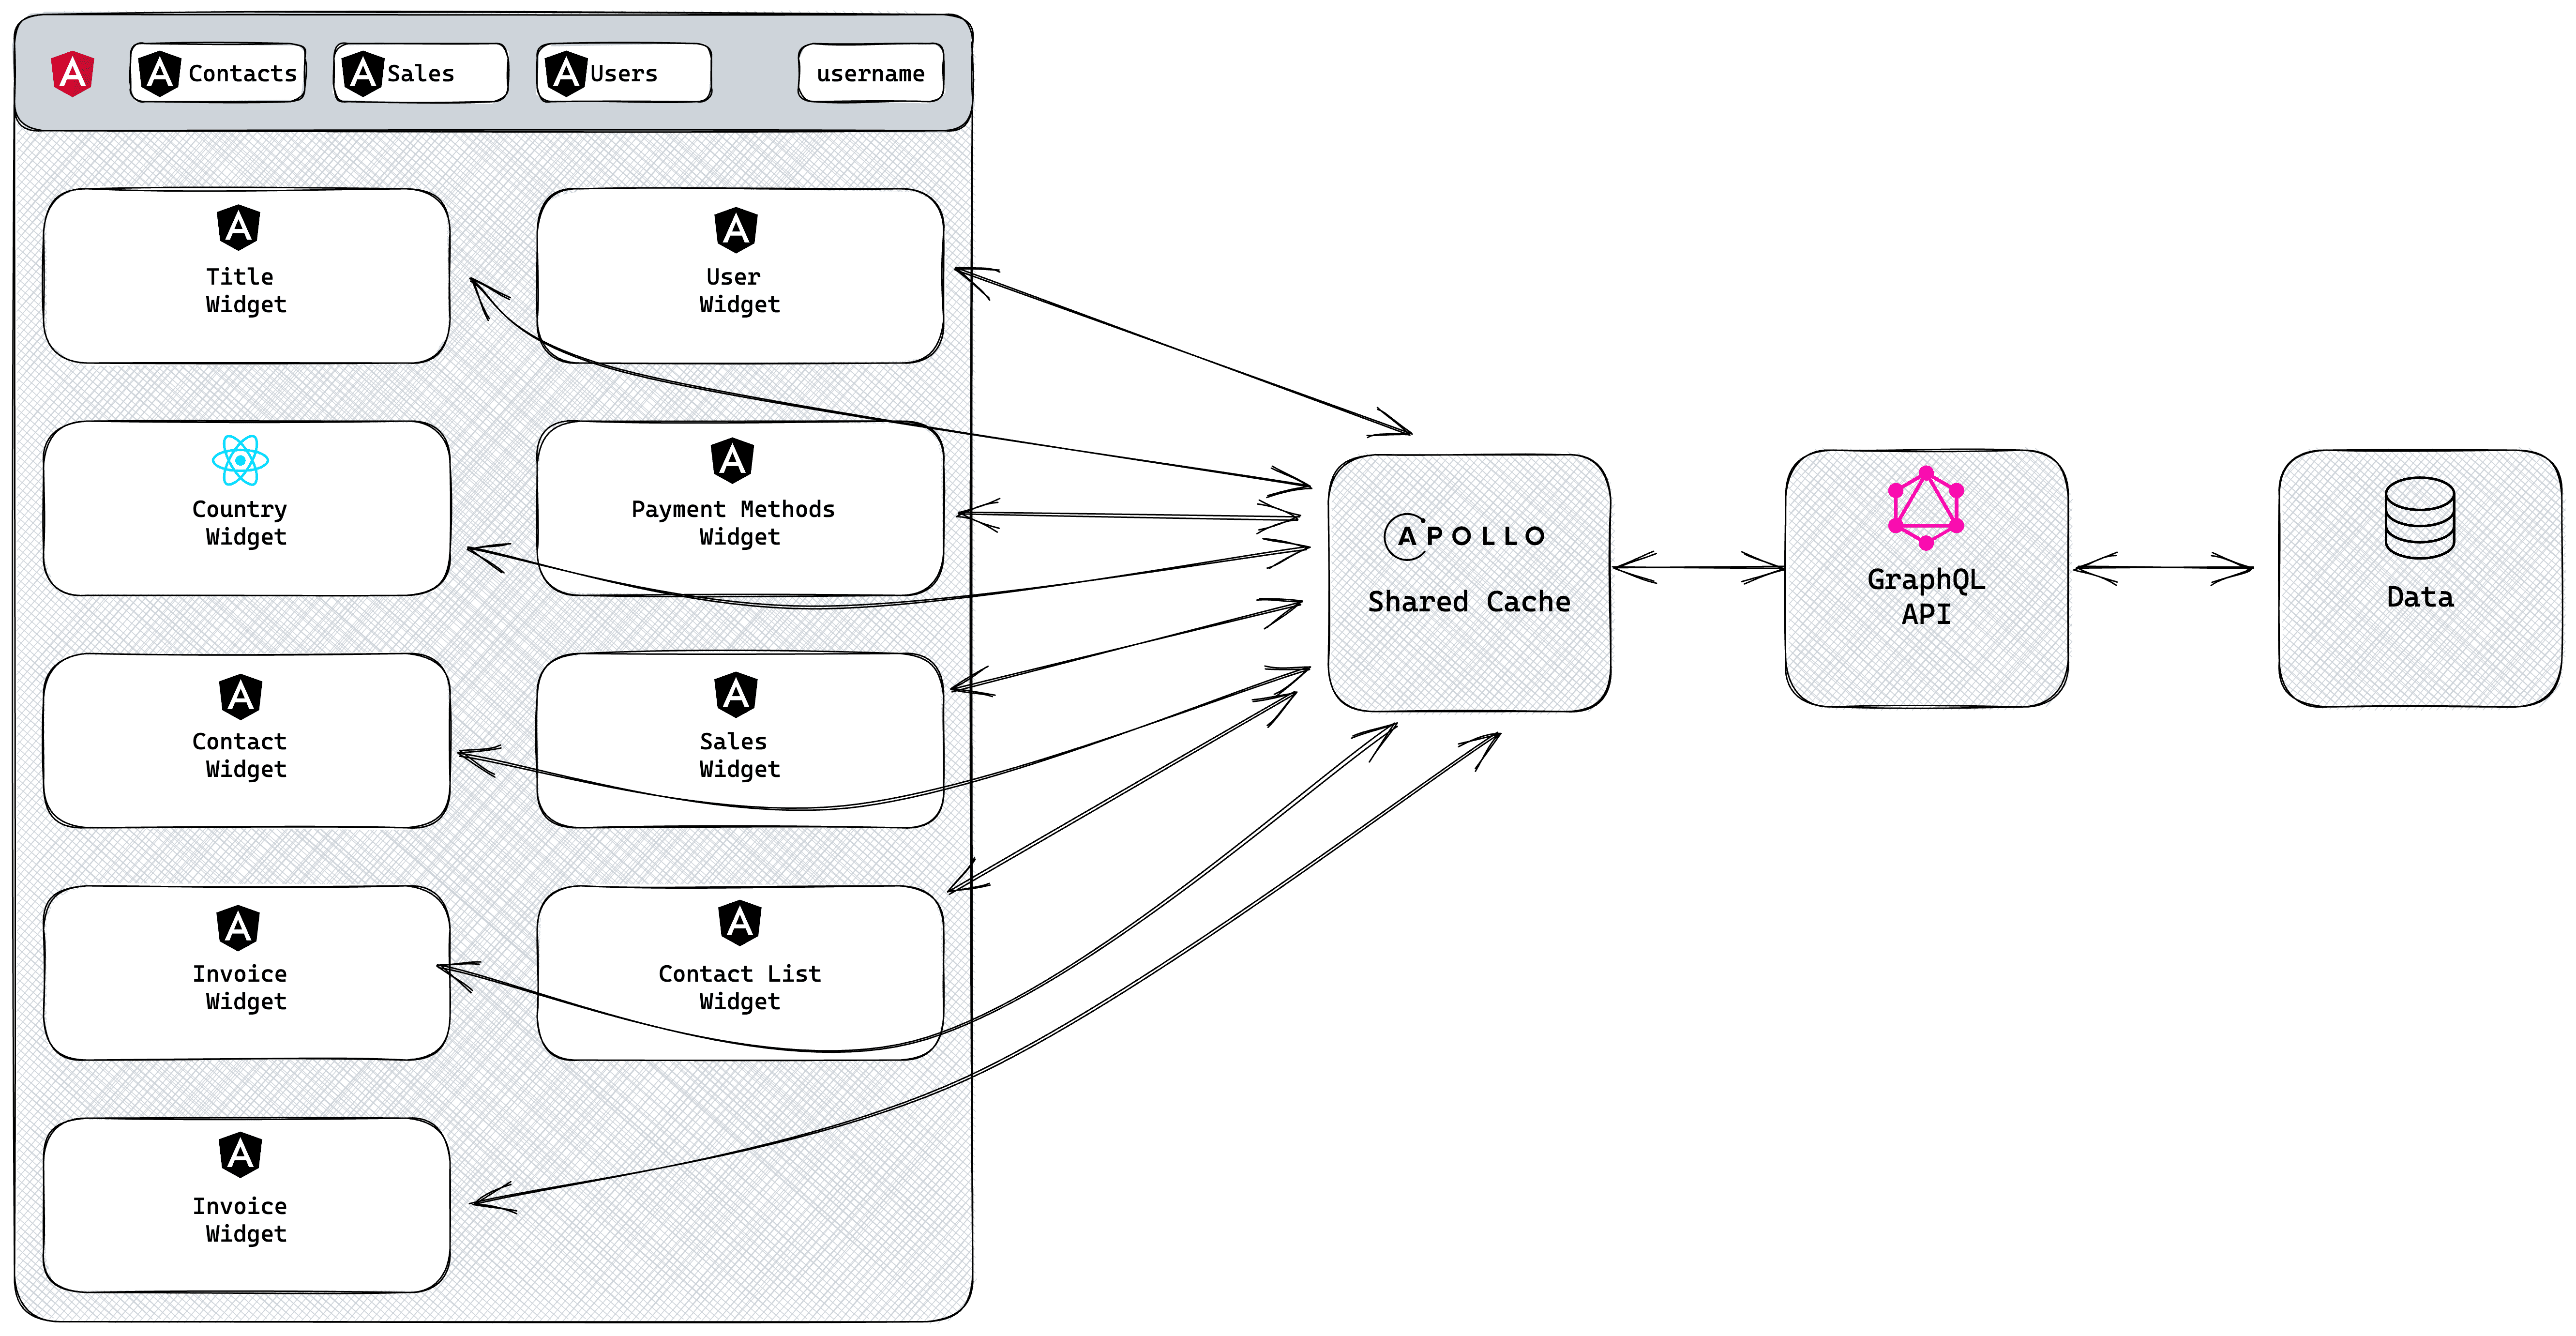
\includegraphics[width=1\linewidth]{images/applied-methods/prototypical-implementation/host-architecture.png}
  \caption{The structure of the micro-frontend prototype.}\label{fig:applied-methods:prototype-micro-frontend-architecture}
\end{figure}
\fi

\noindent Each micro-frontend is deployed separately and is accessible by a separate \ac{URL}. The application shell is the entry point for the client, and it consumes the Dashboard, Contact, Sales, and User application. The main functionality of the micro-frontends is encapsulated in modules. These modules of the applications can be easily accessed through the Module Federation and used by the application shell. The modules are used in exactly the same way in the standalone application.

\bigskip

\noindent The Listing \ref{code:applied-methods:module-federation-config-expose} shows the configuration of the contact micro-frontend to expose its primary implementation through module federation in the form of the \texttt{entry.module}. The configuration of the other micro-frontends looks similar. The properties of the module-federation plugin were already discussed in Section \ref{subsection:background:micro-frontend:module-federation}. All Angular- and Apollo- dependencies are specified to be shared across all micro-frontends. Sharing the dependencies ensures that all micro-frontends use the same and only one version of the dependencies. Listing \ref{code:applied-methods:module-federation-config-expose}, the versions of the dependencies are explicitly specified. Inside the prototype, the versions are read from the root \texttt{package.json} to ensure consistency with the installed versions.

\ifshowListings
\begin{listing}[H]
  \begin{minted}{typescript}
module.exports = {
  name: 'contact',
  exposes: {
    './Module': 'apps/contact/src/app/remote-entry/entry.module.ts',
  },
  shared: [
    '@angular/core': {
      singleton: true, strictVersion: true, requiredVersion: '^15.1.1' 
    },
    ...
    'apollo-angular': { 
      singleton: true, strictVersion: true, requiredVersion: '^4.0.1' 
    },
    ...
  ]
};
  \end{minted}
  \caption{The Module Federation configuration to expose the contact's functionality.}\label{code:applied-methods:module-federation-config-expose}
\end{listing}
\fi

\noindent The application shell is configured to consume the remote modules listed inside the \texttt{remotes}-object. The configuration to consume the four micro-frontends of the architecture can be seen in the Listing \ref{code:applied-methods:module-federation-config-consume}. This configuration allows the application shell to consume the \texttt{entry.module} of the micro-frontend, which was exposed before with the configuration from Listing \ref{code:applied-methods:module-federation-config-expose}. As with the remote module configuration, the application shell shares the same dependencies. Dependency sharing is required so that micro-frontends can load their runtime dependencies from the application shell and use the same dependency version.

\ifshowListings
\begin{listing}[H]
  \begin{minted}{typescript}
module.exports = {
  name: 'host',
  remotes: {
    contact: 'contact@http://localhost:4201/remoteEntry.js'
    sales: 'sales@http://localhost:4202/remoteEntry.js'
    dashboard: 'dashboard@http://localhost:4203/remoteEntry.js'
    user: 'user@http://localhost:4204/remoteEntry.js'
  },
  shared: {
    '@angular/core': {
      singleton: true, strictVersion: true, requiredVersion: '^15.1.1' 
    },
    ...
    'apollo-angular': { 
      singleton: true, strictVersion: true, requiredVersion: '^4.0.1' 
    },
    ...
  }
};
  \end{minted}
  \caption{The configuration of the application shell to be able to consume micro-frontends.}\label{code:applied-methods:module-federation-config-consume}
\end{listing}
\fi

\noindent Using the Module Federation configuration from Listing \ref{code:applied-methods:module-federation-config-consume}, the application shell can load and display the remote modules. Listing \ref{code:applied-methods:angular-route-to-remote-module} shows the route configuration for displaying the contact micro-frontend using Angular's router. Nx offers helper methods like \texttt{loadRemoteModule} for Module Federation to load remote modules into a route of the application shell. The application shell follows the approach of showing one micro-frontend per route. The dashboard on the other hand displays multiple micro-frontend widgets on a page.

\ifshowListings
\begin{listing}[H]
  \begin{minted}{typescript}
const routes: Routes = [
  {
    path: 'contact',
    loadChildren: () => loadRemoteModule('contact', './Module')
      .then((m) => m.ContactRemoteEntryModule),
  },
  ...
]
  \end{minted}
  \caption{An Angular route to the contact application.}\label{code:applied-methods:angular-route-to-remote-module}
\end{listing}
\fi

\ifshowAppliedMethodsCustomNginxConfSection
  \subsection{Deployment problems}\label{subsection:applied-methods:prototypical-implementation:nginx-problems}

Docker is used to run the micro-frontends in production. The Nginx web server in a Docker container is used to deliver the application files to the client. The dockerfile for the micro-frontends is shown in Listing \ref{code:applied-methods:prototype-implementation-dockerfile}. The application to deploy needs to be built before creating the docker image. Afterwards the necessary files are copied into the docker image.

\ifshowListings
  \begin{listing}[H]
  \begin{minted}{dockerfile}
FROM nginx:alpine
COPY nginx/nginx.conf /etc/nginx/nginx.conf
COPY dist/apps/contact/ /usr/share/nginx/html/
    
CMD [
  "/bin/sh", 
  "-c", 
  "envsubst < /usr/share/nginx/html/assets/settings.template.json >" 
  "/usr/share/nginx/html/assets/settings.json && exec nginx -g daemon off;"
]
  \end{minted}
  \caption{The dockerfile for containerizing a micro-frontend.}\label{code:applied-methods:prototype-implementation-dockerfile}
  \end{listing}
\fi

\noindent Module Federation applications expose a file called \texttt{remoteEntry.mjs}, which is consumed by an application shell. However, Nginx currently cannot interpret the mime-type of \texttt{\*.mjs} files which would be \ac{JS}. Therefore, it falls back to the default mime-type \texttt{text/plain}, where \ac{JS} is not executed in the browser. As a workaround for this problem, a custom \texttt{nginx.conf} has been created that sets the default mime-type to \texttt{text/javascript}, which allows the execution of the script in the browser. A part of the configuration is shown in Listing \ref{code:applied-methods:prototype-implementation-custom-nginx-conf}.

\ifshowListings
  \begin{listing}[H]
  \begin{minted}{bash}
default_type text/javascript;
  \end{minted}
  \caption{The custom configuration for Nginx to set the default mime type.}\label{code:applied-methods:prototype-implementation-custom-nginx-conf}
  \end{listing}
\fi

\noindent The custom configuration allows Nginx to correctly load and interpret the remote module files. Setting another default mime type will not break the web server because modern frameworks like Angular just work with \ac{JS} files.

\fi

\subsection{Integrating the React micro-frontend}\label{subsection:applied-methods:prototypical-implementation:react-micro-frontend}

One widget for the dashboard micro-frontend was implemented using the popular frontend framework React. Implementing one micro-frontend in another technology was done to show that the concept of sharing a single cache instance between multiple micro-frontends is technology agnostic. The React widget exposes its functionality like the Angular counterparts through Module Federation. In comparison to Angular, React does not have the concept of modules. Therefore, the functionality of the widget is exported as a simple, functional React component, as shown in listing  \ref{code:applied-methods:module-federation-react-config-expose}.

\ifshowListings
\begin{listing}[H]
    \begin{minted}{typescript}
module.exports = {
  name: 'react-dashboard',
  exposes: { './Module': './src/remote-entry.ts' },
  shared: [
    react: {
      singleton: true, strictVersion: true, requiredVersion: '^18.2.0' 
    },
    ...
  ]
};
    \end{minted}
    \caption{Module Federation config for exposing the \texttt{remote.entry} of the React micro-frontend.}\label{code:applied-methods:module-federation-react-config-expose}
\end{listing}
\fi

\noindent The host application can consume the React application in the same way as the Angular remote modules. However, rendering a React component in an Angular application is natively impossible. Therefore, an Angular wrapper component loads the React remote bundle and renders it inside an HTMLElement. The Angular adapter makes it possible for the Angular router to point to the component, which is impossible with the React component directly.

\bigskip

\noindent Angular modules consumed through Module Federation can access the \ac{DI} tree from the application shell. However, React does not offer a \ac{DI} system like Angular and cannot access the necessary dependencies. React uses contexts to pass down data through the component tree without manually passing properties down level by level. It enables data sharing between components not directly connected in the component tree. The make the shared caching layer inside the React application work, the React widget needs the \texttt{InMemoryCache} instance from the application shell. The shared caching layer is explained in Section \ref{section:applied-methods:shared-caching-layer} in more detail, but the general concept is needed to understand the need to incorporate the instance into the React context. Therefore, the Angular wrapper creates the exposed widget inside a React context provider with the necessary dependencies. The function in listing \ref{code:applied-methods:prototypical-implementation:render-react-component-with-context} shows the React context provider's creation and the React component's rendering. 

\ifshowListings
\begin{listing}[H]
    \begin{minted}{typescript}
render<Comp extends ElementType>(rootEl: Root, Comp: Comp) {
  rootEl.render(
    createElement(
      NgReactContext, {
        ctx: {
          graphQLClientCache: this.injector.get(GRAPHQL_CLIENT_CACHE),
          ...
        },
      },
      createElement(Comp, compProps)
    )
  );
}
    \end{minted}
    \caption{The function to render the React widget into an Angular component.}\label{code:applied-methods:prototypical-implementation:render-react-component-with-context}
\end{listing}
\fi

\noindent With the help of the function, the widget can access the instance of the \texttt{InMemoryCache} from the application shell and use it to share the cache between the Angular and the React micro-frontend. How the \texttt{InMemoryCache} from the application shell is injected and consumed is shown in listing \ref{code:applied-methods:prototypical-implementation:consume-react-context}. The cache is used to create a new instance of the ApolloClient, and afterwards the client is provided to the application using another context.

\ifshowListings
\begin{listing}[H]
    \begin{minted}{typescript}
const injector = useContext(InjectorCtx);

const client = new ApolloClient({
  uri: injector.graphQLEndpoint,
  cache: injector.graphQLClientCache,
  ...
});

return (
  <ApolloProvider client={client}>
    <PaymentMethodList />
  </ApolloProvider>
);

    \end{minted}
    \caption{Use the \texttt{InMemoryCache} instance from the React context.}\label{code:applied-methods:prototypical-implementation:consume-react-context}
\end{listing}
\fi


\subsection{Backend for frontend}\label{subsection:background:prototypical-implemenation:bff}

The \ac{BFF} pattern was implemented using GraphQL. A single \ac{BFF} service is used for all micro-frontends of the architecture. Apollo Server is used as the GraphQL server and was chosen to implement the \ac{API}. Every micro-frontend uses the same \ac{BFF} service, however, multiple GraphQL \acp{API} could be used. Each micro-frontend is a standalone application, therefore it could communicate with multiple GraphQL \acp{API}.
The GraphQL \ac{API} fetches the data from a cluster of microservices and brings the results into the correct shape for the micro-frontends. The GraphQL \ac{API} was developed, while the microservices were still under development. However, the data model was already finalized. Therefore, the GraphQL \ac{API} was implemented using mock data. The mock data was generated using the database schemas of the microservices. The queries and mutations were implemented by directly reading and writing the mock data. Once the microservices are implemented, the GraphQL \ac{API} will be modified to communicate directly with the microservices within the company.


\ifshowAppliedMethodsLoadRemoteSettingsSection
  \subsection{Remote application configuration}\label{subsection:applied-methods:prototypical-implementation
:load-remote-settings}

The application shell is set up to use dynamic Module Federation. The location of the remote applications is determined at runtime. The problem with the so-called static Module Federation is that the \ac{URL} of the remote application must be known at build time. However, this is troublesome if the application should be built once and deployed to multiple stages. It is very cumbersome to build an artifact for every environment.

\bigskip

\noindent One possibility to fetch the remote definitions at runtime is to store them in a simple \ac{JSON} file, which can easily be configured for every environment. The host makes a simple GET request to get the definitions inside the \ac{JSON} file. The content of the file has to be a simple mapping between the name of the remote and their location, as shown in Listing \ref{code:applied-methods:define-module-federation-manifest}.

\ifshowListings
\begin{listing}[H]
\begin{minted}{json}
{
  "sales": "http://localhost:4201",
  "contact": "http://localhost:4202",
  "dashboard": "http://localhost:4203",
  "user": "http://localhost:4204"
}
\end{minted}
\caption{The structure of the micro-frontend definition file with the name and \ac{URL}.}\label{code:applied-methods:define-module-federation-manifest}
\end{listing}
\fi

\noindent The host has to fetch the definitions when starting up the application. The definitions are stored and stored for the Webpack configuration, as shown in Listing \ref{code:applied-methods:load-module-federation-settings}. If the file can be fetched successfully, the bootstrap process of the application gets imported dynamically.

\ifshowListings
\begin{listing}[H]
\begin{minted}{typescript}
fetch('/assets/module-federation.manifest.json')
  .then((res) => res.json())
  .then((definitions) => setRemoteDefinitions(definitions))
  .then(() => import('./bootstrap').catch((err) => console.error(err)));
\end{minted}
\caption{Loading the micro-frontend definition file during initialization.}\label{code:applied-methods:load-module-federation-settings}
\end{listing}
\fi

\noindent Another use case for dynamic content is the configuration of an application. This configuration includes the endpoint of the GraphQL \ac{API}, which can be different in staging and production. Therefore, the configuration should also be fetched dynamically. The settings are fetched during the first load of the application and stored for later use. The configuration is stored inside a file called \texttt{settings.json}, served alongside the application. Angular provides a handy mechanism to run code when the application is loaded.

\bigskip

\noindent With the help of the \texttt{APP\_INITIALIZER} injection token, asynchronous code can be executed when the application starts up. Such tasks include fetching data from a remote \ac{API} and setting up configuration or initializing third-party libraries. When an Angular app starts, it will execute all the functions registered with \texttt{APP\_INITIALIZER} in the order they were defined. If one of the initialization tasks fails, the application will not load. \cite{misc:-:applied-methods:prototype-implementation:angular-app-initializer}

\bigskip

\noindent The Listing \ref{code:applied-methods:fetch-and-store-settings} shows a simplified version to fetch and store the settings in the local storage. The settings are fetched from the \texttt{settings.json} file, which content is used to configure the application. The settings of the application shell are stored with the key \texttt{host}. Each application of the micro-frontend architecture stores its settings with its application name as the key.

\ifshowListings
\begin{listing}[H]
\begin{minted}{typescript}
@NgModule({
  providers: [{
    provide: APP_INITIALIZER,
    async useFactory(http: HttpClient, storage: StorageClient) {
      const environmentConfig = await lastValueFrom(
        http.get('assets/settings.json')
      );
      storage.store('host', environmentConfig);
    },
    multi: true,
    deps: [HttpClient, StorageClient],
  }]
})
class CoreModule {}
\end{minted}
\caption{Fetch \& store the settings of the application shell.}\label{code:applied-methods:fetch-and-store-settings}
\end{listing}
\fi

\subsubsection{Loading the configuration of the remote applications}\label{subsubsection:applied-methods:prototypical-implementation
:load-the-configuration}

Each application of the prototypical micro-frontend architecture follows this approach. When the application is initialized, the application configuration is fetched with a GET request from the \texttt{settings.json}. As mentioned in the previous section, each micro-frontend stores its settings with the application's name as the key. However, the configuration does not get fetched when the application shell consumes the functionality of a micro-frontend. Therefore, the application throws errors because they cannot access their settings from the storage. To solve the problem of missing settings for the application, the configuration of a remote application is fetched and stored inside a store when the user navigates to it. This procedure is explained visually in Figure \ref{fig:applied-methods:load-remote-settings}.

\ifshowImages
  \begin{figure}[H]
  \centering
  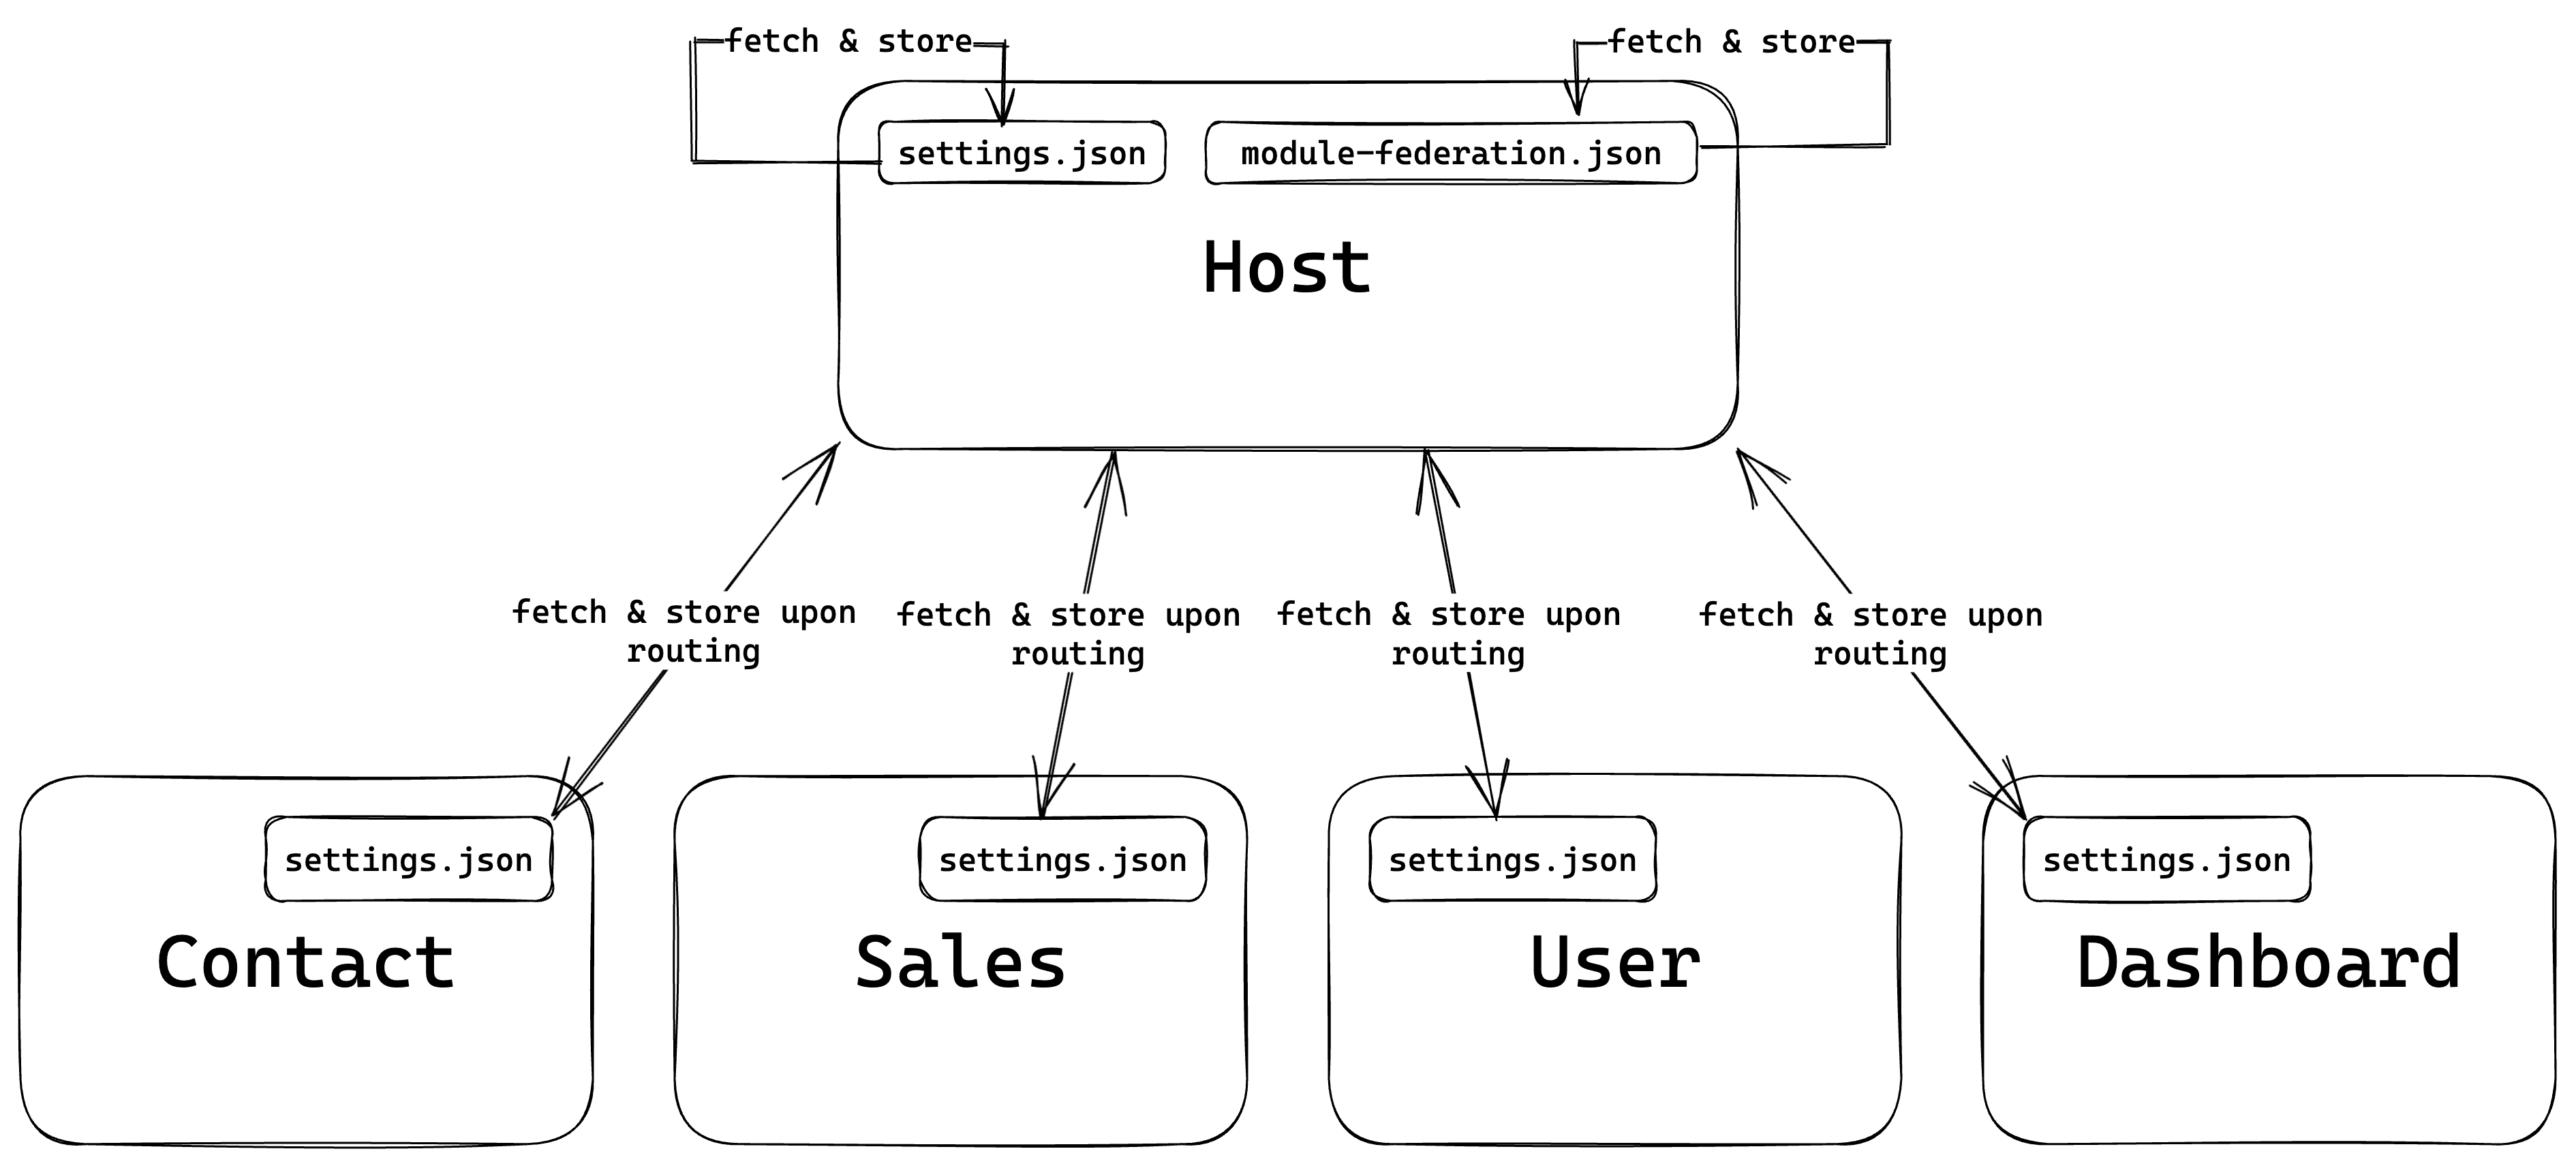
\includegraphics[width=0.9\linewidth]{images/applied-methods/prototypical-implementation/load-remote-settings.png}
  \caption{Loading a storing the configuration of the remote applications.}\label{fig:applied-methods:load-remote-settings}
  \end{figure}
\fi

\noindent With the help of Angular resolvers, the resolvers executed before the components of the target are rendered. Due to the dynamic Module Federation, the location of the remote module is known. Therefore, the \texttt{settings.json} is loaded and stored in addition to loading the remote module. A simplified version of the code is shown in Listing \ref{code:applied-methods:fetch-and-store-remote-application-settings}. The same principle applies to every remote module, which is consumed.

\ifshowListings
\begin{listing}[H]
\begin{minted}{typescript}
const routes: Routes = [{
    path: 'contact',
    loadChildren: () => loadRemoteModule('contact', './Module')
      .then((m) => m.ContactRemoteEntryModule),
    resolve: {
      settings: () => {
        const contact = inject(StorageClient).get('manifest')['contact'];
        return inject(HttpClient).get(`\${contact}/assets/settings.json`);
      }
    },
  },
  ...
]
\end{minted}
\caption{Fetch the settings of the contact application.}\label{code:applied-methods:fetch-and-store-remote-application-settings}
\end{listing}
\fi

\noindent With this approach, each application can access its settings like running in standalone mode. Moreover, it has another benefit because each application can only access its settings and not the settings of the other applications. 

\fi

\ifshowAppliedMethodsSecondaryEntrypoints
  \subsection{Sharing secondary entry points}\label{subsection:applied-methods:prototypical-implementation:sharing
-secondary-entrypoints}

By default, all dependencies of the micro-frontends are shared through Module Federation. The configuration options for every dependency are \texttt{singleton}-, \texttt{strictVersion}-, and \texttt{requiredVersion}-property. These properties are explained in more detail in Section \ref{subsection:background:micro-frontend:module-federation}. The versions of these dependencies are determined automatically from the \texttt{package.json}. However, not all packages support being shared with these default settings. The npm package \texttt{@apollo/client} has a problem because it has secondary entry points. When trying to share \texttt{@apollo/client/core}, \texttt{@apollo/client/link/batch} and \texttt{@apollo/client/link/error} the error message in Figure \ref{fig:applied-methods:sharing-secondary-entrypoints-error} is shown.

\ifshowImages
  \begin{figure}[H]
  \centering
  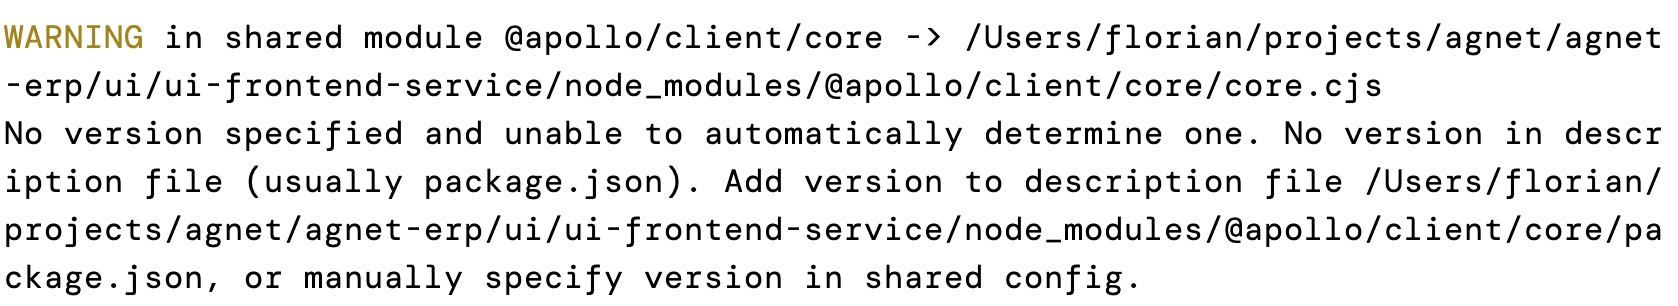
\includegraphics[width=1\linewidth]{images/applied-methods/prototypical-implementation/module-federation-apollo-warning.jpg}
  \caption{A Module Federation warning, when the dependency \texttt{@apollo/client} should be shared.}\label{fig:applied-methods:sharing-secondary-entrypoints-error}
  \end{figure}
\fi

\noindent The problems are secondary entry points like \texttt{@apollo/client/core}, which are a bit like an npm package in another npm package. The \texttt{package.json} of \texttt{@apollo/client/core} is shown in Listing \ref{code:applied-methods:package-json-apollo-client-core}. Webpack tries to resolve the version of the secondary entry point from the \texttt{package.json} and not from \texttt{@apollo/client}. Therefore, it cannot determine the version and prints the warning shown in Figure \ref{fig:applied-methods:sharing-secondary-entrypoints-error}. The warning does not lead to an error, but these dependencies cannot be shared and must be included in every micro-frontend bundle.

\ifshowListings
\begin{listing}[H]
  \begin{minted}{json}
{
  "name": "@apollo/client/core",
  "type": "module",
  "main": "error.cjs",
  "module": "index.js",
  "types": "index.d.ts",
  "sideEffects": false
}
  \end{minted}
  \caption{The \texttt{package.json} of \texttt{@apollo/client/core}.}\label{code:applied-methods:package-json-apollo-client-core}
\end{listing}
\fi

\noindent The Module Federation was fixed by specifying the version for these packages manually. The version is the same as that of \texttt{@apollo/client}. The configuration for the sharing of these packages is shown in the Listing \ref{code:applied-methods:sharing-secondary-entrypoints-config}. 

\ifshowListings
\begin{listing}[H]
  \begin{minted}{typescript}
shared: (libraryName, defaultConfig) => {
  if (libraryName.includes(`@apollo/client/`))
    return { ...defaultConfig, version: '^3.6.9' };

  return defaultConfig;
}
  \end{minted}
  \caption{Specify the version for the secondary entry points for the \texttt{@apollo/client} package.}\label{code:applied-methods:sharing-secondary-entrypoints-config}
\end{listing}
\fi

\fi
\section{Communication from the shell- to the remote-application}\label{section:methods:communication-shell-remote}

To solve the problem of building a common caching layer, some form of communication between the shell and remote application had to be implemented. To ensure that the micro-frontends remain independent of each other, it should be avoided that they communicate directly with each other.

Angular provides a great tool for this use case, namely dependency injection. The shell application can provide services that can later be injected by the remote applications. This is very handy because the micro frontend can provide the same services as the shell application in standalone mode. Therefore, the remote module can be easily used within the remote and shell application.

For example i implemented a layout-service that takes advantage of dependency injection.

\ifshowImages
\begin{figure}[H]
\centering

\includegraphics[width=1\linewidth]{images/prototype-screenshots/contact-header.png}
\caption{Beispiel für die Beschriftung eines Buchrückens.}
\end{figure}
\fi

\ifshowImages
\begin{figure}[H]
\centering
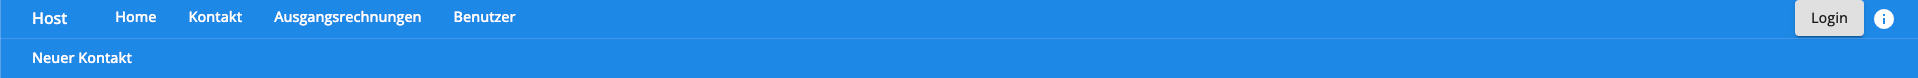
\includegraphics[width=1\linewidth]{images/prototype-screenshots/host-contact-header.png}
\caption{Beispiel für die Beschriftung eines Buchrückens.}
\end{figure}
\fi

\section{Shared caching layer}\label{section:applied-methods:shared-caching-layer}

The previous section explained how the communication strategy within the micro-frontend architecture works behind the scenes. Apollo Client's caching mechanism should be used to boost the performance of the micro-frontend architecture and handle the problems of over-fetching and over-requesting. This section goes into more detail, how the shared caching layer is implemented and integrated into the architecture. The structure of the shared caching layer is shown in Figure \ref{fig:applied-methods:structure-shared-caching-layer}. Each micro-frontend has a separate instance of the Apollo Client, but they should all use the same instance of the \texttt{InMemoryCache}. Therefore, each application can provide its own configuration for the Apollo Client, however all micro-frontend use the same instance of the \texttt{InMemoryCache}. The \texttt{InMemoryCache} stores the results of GraphQL queries. When a micro frontend needs to retrieve a query that is already cached, it can reuse the data that is already cached instead of retrieving it again from the GraphQL \ac{API} again. This caching strategy reduces the number of network requests and thus the amount of data that has to be transferred over the network.

\ifshowImages
  \begin{figure}[H]
  \centering
  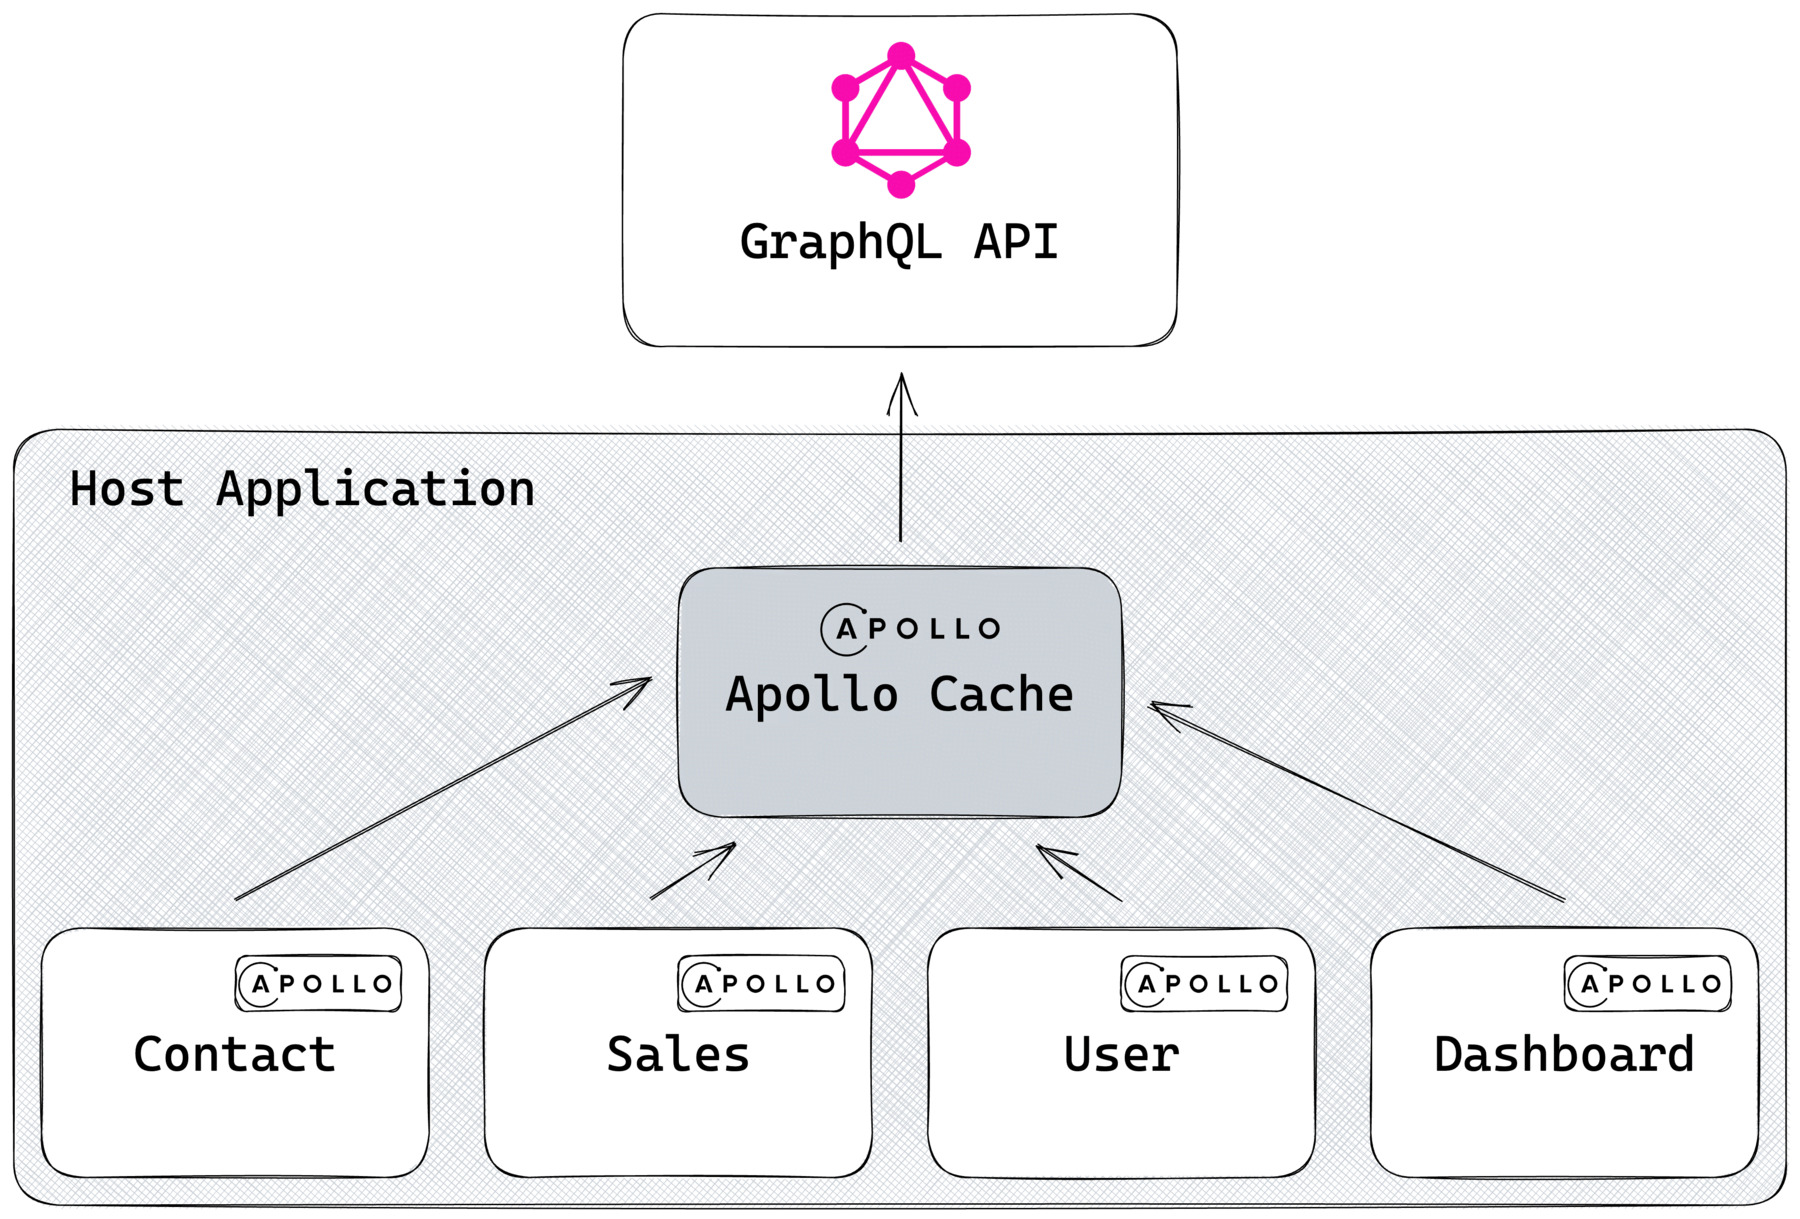
\includegraphics[width=0.7\linewidth]{images/applied-methods/shared-caching-layer/shared-caching-layer.jpg}
  \caption{The structure of the shared caching layer.}\label{fig:applied-methods:structure-shared-caching-layer}
  \end{figure}
\fi

\noindent The application shell must provide the instance of the GraphQL \texttt{InMemoryCache} to make sure that all micro-frontends have the same instance. Listing \ref{code:applied-methods:creating-the-apollo-client} shows how the Apollo Client is created for an Angular application with default settings. The \texttt{cache} property is important, as it needs an instance of Apollo's \texttt{InMemoryCache}. This allows for the architecture to create a single cache instance elsewhere and pass it to the Apollo Client. 

\ifshowListings
\begin{listing}[H]
\begin{minted}{typescript}
@NgModule({
  imports: [ApolloModule],
  providers: [{
    provide: APOLLO_OPTIONS,
    useFactory: (httpLink: HttpLink) => ({
      cache: new InMemoryCache(),
      link: httpLink.create({ uri: 'http://localhost:3000' }),
    }),
    deps: [HttpLink],
  }]
})
class AppModule {}
\end{minted}
\caption{Create a new instance of the Apollo Client.}\label{code:applied-methods:creating-the-apollo-client}
\end{listing}
\fi

\noindent The concept behind the shared caching layer is to instantiate the cache instance inside the application shell and provide it to the micro-frontends. The instance of the \texttt{InMemoryCache} should be injectable through an injection token, just like the injection token from Section \ref{section:applied-methods:communication-shell-remote}, which specifies whether the application runs in standalone mode. The injection token can be provided by the application shell and injected and used by the micro-frontends. Moreover, the application itself can provide the instance of the cache when it runs in standalone mode. The \texttt{GRAPHQL\_CLIENT\_CACHE} token can be used to provide an instance of Apollo's \texttt{InMemoryCache} to the micro-frontends, as shown in Listing \ref{code:applied-methods:graphql-client-cache-provider}.

\ifshowListings
\begin{listing}[H]
\begin{minted}{typescript}
@NgModule({
  providers: [
    { provide: GRAPHQL_CLIENT_CACHE, useValue: new InMemoryCache() }
  ]
})
class HostCoreModule {}
\end{minted}
\caption{Provide the instance of the \texttt{InMemoryCache} to \ac{DI}.}\label{code:applied-methods:graphql-client-cache-provider}
\end{listing}
\fi

\subsection{GraphQL Client creation}{subsection:applied-methods:shared-caching-layer:graphql-client-creation}

\noindent The prototype provides abstractions to create the necessary configuration for using the Apollo Client more easily and identically for all micro-frontends. Listing \ref{code:applied-methods:graphql-client-creation} shows the usage of the abstraction to create a new instance of Apollo Client for a micro-frontend. The module \texttt{GraphQLClientOptionsModule} hides the complexity of creating and providing a Apollo Client instance, as shown in Listing \ref{code:applied-methods:creating-the-apollo-client-with-a-shared-cache}. The moduls has a required parameter that specifies a unique name. This name is used to identify and track active Apollo Clients inside the architecture. The \texttt{GraphQLClientOptionsModule} should be used in every module that needs GraphQL functionality and is exposed through Module Federation. When the micro-frontend is then integrated within the application shell, it has its own instance of the Apollo Client. This facilitates independent development of micro-frontends, as the Apollo Client configuration remain the same whether it is running in standalone mode or consumed by the application shell. For example, a problem could arise if the application shell provides the instance of the Apollo Client and the contact micro-frontend injects that instance with \ac{DI}. The contact development team might configure the Apollo Client differently within the contact application, and the functionality might not work as expected within the application-shell because the configuration might be different.

\ifshowListings
  \begin{listing}[H]
    \begin{minted}{typescript}
@NgModule({
  imports: [ GraphQLClientOptionsModule.withConfig('contact-remote') ]
})
class ContactRemoteCoreModule {}
  \end{minted}
  \caption{Create the Apollo Client instance for the micro-frontend.}\label{code:applied-methods:graphql-client-creation}
  \end{listing}
\fi

\ifshowListings
\begin{listing}[H]
\begin{minted}{typescript}
@NgModule({
  imports: [ApolloModule],
  providers: [{
    provide: APOLLO_OPTIONS,
    useFactory(httpLink: HttpLink, cache: InMemoryCache) {
      const link = httpLink.create({uri: 'http://localhost:3000'});
      return { cache, link };
    },
    deps: [HttpLink, GRAPHQL_CLIENT_CACHE],
  }]
})
class ContactRemoteModule {}
\end{minted}
\caption{Access the shared \texttt{InMemoryCache} instance from \ac{DI}.}\label{code:applied-methods:creating-the-apollo-client-with-a-shared-cache}
\end{listing}
\fi

\noindent The \texttt{GraphQLClientOptionsModule} uses the storage service to get the required configuration for the Apollo Client. For example, \ac{URL} of GraphQL \ac{API} is taken from the storage service. By default, it tries to inject the \texttt{GRAPHQL\_CLIENT\_CACHE}, and use it as the cache instance for the Apollo Client. If it cannot be injected, a separate cache instance is created for the client. An addtional injection token \texttt{GRAPHQL\_CLIENT\_OPTIONS\_CONFIG} can be used to specify additional options for creating a new Apollo Client instance. The injection token's usage and default options are shown inside Listing \ref{code:applied-methods:graphql-client-extra-configuration-options}. The injection token must be provided inside the same module where the \texttt{GraphQLClientOptionsModule} was defined.

\ifshowListings
\begin{listing}[H]
\begin{minted}{typescript}
@NgModule({
  providers: [{
    provide: GRAPHQL_CLIENT_OPTIONS_CONFIG,
    useValue: {
      shareCache: true,
      persistCache: false,
      useTypePolicies: true,
      typePolicies: CONTACT_TYPE_POLICIES,
    },
  }]
})
class ContactRemoteCoreModule {}
\end{minted}
\caption{Provide additional options for creating the Apollo Client instance.}\label{code:applied-methods:graphql-client-extra-configuration-options}
\end{listing}
\fi

\noindent The options include \texttt{shareCache}, \texttt{persistCache}, \texttt{useTypePolicies} and \texttt{typePolicies}. The \texttt{shareCache} setting is used to specify whether the Apollo Client should use the \texttt{InMemoryCache} instance provided by \texttt{GRAPHQL\_CLIENT\_CACHE} or if it should create a new instance, specifically for this remote module. The \texttt{persistCache} option is set to \texttt{false} by default. It stores the contents of the \texttt{InMemoryCache} inside the \texttt{localStorage}. This feature provided by the Apollo Client allows faster initial page renders, because the data from the \texttt{localStorage} is transferred back to the cache when the application is loaded. The options \texttt{useTypePolicies} and \texttt{typePolicies} are used together and must be specified together. The property \texttt{useTypePolicies} specifies whether the type policies from the option \texttt{typePolicies} should be used or not. Type policies allow Apollo Client to customize the read and write operations of every field inside the cache. They are explained in more detail in Section \ref{subsubsection:background:graphql:apollo-server-client:type-policies}. As explained earlier, each micro-frontend has its own Apollo client instance with a shared cache instance, so the type policies cannot be registered directly when the \texttt{InMemoryCache} is created. The option \texttt{typePolicies} has the same type as the \texttt{typePolicies} parameter of the \texttt{InMemoryCache} constructor. Specifying the option when providing the \texttt{GRAPHQL\_CLIENT\_OPTIONS\_CONFIG} allows the micro-frontend to specify additional type policies for the cache. Part of the code to create the shared cache and append type-policies within the \texttt{GraphQLClientOptionsModule} is shown in Listing \ref{code:applied-methods:adding-extra-type-policies}. First, the instance of the cache should be injected. If the cache cannot be injected, it means that the Apollo Client has to create a new instance of the \texttt{InMemoryCache}. The \texttt{typePolicies} are added to the cache instnace if both options \texttt{typePolicies} and \texttt{useTypePolicies} are truthy values.

\ifshowListings
\begin{listing}[H]
\begin{minted}{typescript}
const cache = inject(GRAPHQL_CLIENT_CACHE, { optional: true });
const { shareCache, useTypePolicies, typePolicies } = graphQLClientOptions;

const cacheInstance = shareCache ? cache : new InMemoryCache();

if (typePolicies && useTypePolicies)
  clientCache.policies.addTypePolicies(typePolicies);
\end{minted}
\caption{Insert additional type policies into the cache instance.}\label{code:applied-methods:adding-extra-type-policies}
\end{listing}
\fi

\section{Built a mechanism that reduces the size of queries}\label{section:applied-methods:query-reduction}

After implementing the shared caching layer, the next step was to improve the performance of the micro-frontends by optimizing the use of the cache. The size of the network requests can be reduced by removing parts of a query that are already inside the cache. The theory behind removing fields from the query was already explained in Section \ref{subsection:background:graphql:query-reduction}. The Apollo Client does not provide such a functionality out of the box, but many users request the feature in Apollo's Github Repository. Section \ref{subsubsection:background:graphql:apollo-server-client:in-memory-cache-working} explains how the \texttt{InMemoryCache} of Apollo Client works in more detail. Briefly summarized the caching works with the name and the parameters of a GraphQL query. For example, if a query is executed against the GraphQL \ac{API}, the results of the query are cached. If the same query with the same fields is executed again with the same parameters, the results are fetched from the Apollo Client cache. If the query fetches an additional field, not inside the cache, the complete query is sent to the GraphQL \ac{API}. Only if the queried fields are identical the cache data is used. Consequently, identical queries that fetch different fields are always fetched from the server.

\bigskip

\noindent Consider Listing \ref{code:applied-methods:compare-allusers-user-query}, where the left query fetches all users, and the query on the right fetches a user by its id. Both queries fetch the same data type and the same fields, but they are fundamentally different queries. They have different names and different parameters. Both queries are sent to the GraphQL \ac{API}. The query on the right could be omitted if the user with the given id is fetched from the cache. If the left query is executed before the query on the right, the data to resolve the query on the right could be taken entirely from the cache.

\ifshowListings
\begin{listing}[H]
\begin{minted}{typescript}
query allUsers {                        query user(id: ID!) {
  allUsers {                              user(id: \$id) {
    id                                      id
    username                                username
    email                                   email
    firstName                               firstName
    secondName                              secondName
  }                                       }
}                                      }
\end{minted}
\caption{Comparison between the \texttt{allUsers} and \texttt{User} query.}\label{code:applied-methods:compare-allusers-user-query}
\end{listing}
\fi

\noindent Apollo offers a solution to tackle this problem. The application might have a detail view and a list view that query the same data as in Listing \ref{code:applied-methods:compare-allusers-user-query}. The user query data might already be in the cache, but the Apollo Client does not know that. Therefore, the cache lookup can be configured so the Apollo Client knows where to look for the data. A basic understanding of type policies is needed to understand the cache redirection, described in more detail in Section \ref{subsubsection:background:graphql:apollo-server-client:type-policies}.

\bigskip

\noindent A field policy \texttt{read} function must be written for the user query to inform the Apollo Client where to look for the cached \texttt{User} object. Like the \texttt{firstName} being a \texttt{User} type field, the user query is a field of the root query. This hierarchy resembles the structure of the GraphQL Schema, where the queries have to be defined inside the \texttt{Query} type. Listing \ref{code:applied-methods:query-reduction:graphql-schema} shows an excerpt from the GraphQL schema. All queries that a client can execute are listed inside the \texttt{Query} type.

\ifshowListings
\begin{listing}[H]
\begin{minted}{typescript}
type Query {
  user(id: ID!): User
  allUsers(page: Int, perPage: Int): [User]
  ...
}

type User {
  id: ID!
  firstName: String!
  secondName: String!
  ...
}
\end{minted}
\caption{An excerpt from the GraphQL schema.}\label{code:applied-methods:query-reduction:graphql-schema}
\end{listing}
\fi


\noindent Listing \ref{code:applied-methods:query-reduction:user-cache-redirect} shows the \texttt{read} field policy for the \texttt{User}. Like in the GraphQL schema from Listing \ref{code:applied-methods:query-reduction:graphql-schema}, the user query is a field of the root query. Therefore, the read function is executed every time the client runs the user query. The \texttt{toReference} function is used to cache a reference for a \texttt{User} type. The reference is generated based on its \texttt{\_\_typename} and \texttt{id}, as explained in Section \ref{subsubsection:background:graphql:apollo-server-client:data-normalization}. Apollo Client uses the result of \texttt{toReference} to look up the object in its cache and return it if it is present. The query is sent to the GraphQL \ac{API} if the object is not in the cache.

\ifshowListings
\begin{listing}[H]
\begin{minted}{typescript}
new ApolloClient({
  cache: new InMemoryCache({ typePolicies: { Query: { fields: {
    User: {
      read(_, { args, toReference }): {
        return toReference({ __typename: 'User', id: args.id });
      }
    }
  }}}})
});
\end{minted}
\caption{Writing a cache-redirect for the User-type.}\label{code:applied-methods:query-reduction:user-cache-redirect}
\end{listing}
\fi

\noindent Using cache redirects to reduce the amount of network requests works, but all of the query's requested fields must be already present in the cache. If the user query fetches any field that the allUsers query did not, Apollo Client considers the cache hit incomplete, and the query is executed over the network. That a detail view and a list view are perfectly identical is very rare in applications. Therefore, this approach cannot effectively reduce the size of network requests. Moreover, the approach is very verbose because a redirect has to be written for every data type. The approach does not scale; the same type-policies must be written and registered for every micro-frontend.

\bigskip

\noindent The open-source project \href{https://github.com/appmotion/apollo-augmented-hooks}{apollo-augmented-hooks} on GitHub provides drop-in replacements for Apollo's GraphQL query methods. It provides the functionality to remove fields from a query already in the cache. However, the big problem is that the project was developed specifically for React's Apollo Client. The dependencies were outdated, and the latest release of the library was in 2021. The library's functionality could only be tested with an old Apollo Client and React version. The dependency offered the functionality to remove fields in the cache from a previous GraphQL query. The Apollo-augmented-hooks dependency was forked to use the functionality of the library inside the prototypical micro-frontend architecture. The first step was to update the dependencies to make it work with the latest version of Apollo Client. The problem with the old implementation is that it just supports React's Apollo Client with its hooks. The core functionality of the library was extracted, and an adapter for React and Angular was written utilizing the functionality. The functions have the same \ac{API} as Apollo's original methods, so migration to the new functions is straightforward. The library's functionality was rewritten with \ac{TS}, adding additional features that utilize the cache even more. The implementation is detailed further in Section \ref{subsection:applied-methods:query-reduction:how-does-the-library-work}.

\ifshowAppliedMethodsTestingQueryReduction
  \subsection{Implementing a query reduction testing layer}\label{subsection:applied-methods:query-reduction:testing-query-reduction}

The following abstraction, seen in Listing \ref{code:applied-methods:query-reduction:graphql-client} for the GraphQL client, was created to compare the Apollo Client's default behavior with the improved behavior of reducing queries.The \texttt{watchQuery} and \texttt{mutate} functions have the same \ac{API} as Apollo Client's original query and mutate functions. Two implementations (\texttt{ReduceGraphQLClientImpl}, \texttt{GraphQLClientImpl}) were created for the base class \texttt{GraphQLClient}. The \texttt{ReduceGraphQLClientImpl} uses query reduction, while \texttt{GraphQLClientImpl} utilizes the original Apollo Client functions. A switch is used to determine which implementation is created at runtime.

\ifshowListings
\begin{listing}[H]
\begin{minted}{typescript}
abstract class GraphQLClient {
  abstract watchQuery<TData, TVariables>(
    options: WatchQueryOptions<TData, TVariables>
  ): Observable<QueryResult<TData>>;

  abstract mutate<TData, TVariables>(
    options: MutationOptions<TData, TVariables>
  ): Observable<MutationResult<TData>>;
}
\end{minted}
\caption{The abstract base class for the GraphQL client.}\label{code:applied-methods:query-reduction:graphql-client}
\end{listing}
\fi

\noindent The switch is implemented as a \ac{DI} token, which can be specified in the applications. The \texttt{REDUCE\_QUERY\_OPTIONS} injection token determines whether the query reduction should be used. The usage of the token is shown in the Listing \ref{code:applied-methods:query-reduction:switch-between-apollo-client-and-query-reduction}. The switch decides whether the \texttt{ReduceGraphQLClientImpl} or \texttt{GraphQLClientImpl} is created. The \texttt{ReduceGraphQLClientImpl} is created when the \texttt{reduceQueries} property is set to \texttt{true}. The provider is specified inside the core module of the application to create the provider globally.

\ifshowListings
\begin{listing}[H]
\begin{minted}{typescript}
const REDUCE_QUERY_OPTIONS = 
  new InjectionToken<ReduceQueryOptions>('reduce-query-options');

@NgModule({
  providers: [{
    provide: REDUCE_QUERY_OPTIONS,
    useValue: { reduceQueries: true },
  }]
})
class ContactCoreModule {}
\end{minted}
\caption{Specify whether queries should be reduced.}\label{code:applied-methods:query-reduction:switch-between-apollo-client-and-query-reduction}
\end{listing}
\fi


\fi

\subsection{Query reduction mechanism}\label{subsection:applied-methods:query-reduction:how-does-the-library-work}

This section briefly describes how the query reduction functionality removes fields from the query using the \texttt{InMemoryCache}. Apollo Client allows specifying multiple configuration options when fetching a query from a GraphQL \ac{API}. Three important options are \texttt{variables}, \texttt{query}, and \texttt{fetchPolicy}. The \texttt{query} specifies the GraphQL query, and the \texttt{variables} are the variables for the query. The fetch policy lets the client specify how data is stored and retrieved from the cache. The typical structure of a GraphQL query inside the micro-frontend architecture is shown in Listing \ref{code:applied-methods:query-reduction:executing-graphql-query}. The query fetches the user's details with the given \texttt{id}. The default fetch policy of a query is \texttt{cache-first}.

\ifshowListings
\begin{listing}[H]
\begin{minted}{typescript}
this.graphQLClient.watchQuery({
  variables: { id: `36bad921-8fcf-4f33-9f29-0d3cd70205c8` },
  query: USER_BY_ID_QUERY,
  fetchPolicy: 'cache-first',
});
\end{minted}
\caption{Defining and running a GraphQL query with Apollo Client.}\label{code:applied-methods:query-reduction:executing-graphql-query}
\end{listing}
\fi

\noindent The Apollo Client offers several fetch policies that customize how the client retrieves data from the cache. The available fetch policies are: \cite{misc:-:applied-methods:query-reduction:apollo-client:queries}

\begin{itemize}
  \item \textbf{cache-first (default)}: This fetch policy instructs the Apollo Client first to check the local cache for the query result. If the data is present in the cache, it is returned immediately. Otherwise, Apollo Client will execute the query and fetch the result from the server, which will then be cached.
  \item \textbf{cache-and-network}: This fetch policy combines the cache-first and network-only policies. Apollo Client first checks the cache for the query result and returns it immediately if it is present. Then, a network request is made to fetch the most up-to-date data, which is then used to update the cache. This fetch policy is a good option for displaying data that gets updated frequently.
  \item \textbf{cache-only}: This fetch policy tells Apollo Client only to check the cache for the query result. If the result is present in the cache, it is returned immediately.
  \item \textbf{network-only}: This fetch policy instructs Apollo to skip the cache entirely and always fetch the query result from the server.
  \item \textbf{no-cache}: This fetch policy skips the cache entirely and always fetches the query result from the server. Unlike network-only, the result is not cached.
\end{itemize}

\noindent The first step of the function is whether the fetch policy allows the query to be reduced. Suppose the query is executed with one of the following cache policies: \texttt{cache-only}, \texttt{network-only}, and \texttt{no-cache}; reducing the query is counterproductive. With \texttt{network-only}, the latest data should be fetched from the GraphQL \ac{API}. The \texttt{cache-only} policy only targets the cache; therefore, no reduction is necessary. The no-cache policy bypasses the cache and requests data from the GraphQL \ac{API}. Another feature of Apollo Client is polling. Polling in Apollo Client is a technique used to fetch a query's data at a specified interval periodically, and it allows a near-real-time synchronization with the server. To enable polling for a query, pass a \texttt{pollInterval} (ms) configuration option to the \texttt{watchQuery} method. Removing fields from a query that uses polling does not make sense either because real-time data should be rendered. The following sections describe the steps needed to reduce the query.

\subsubsection{Identify key fields of every GraphQL type}

The first step is identifying the key fields of the types inside the schema. The contents of the \texttt{InMemoryCache} can be extracted using the \texttt{cache.extract()} function. This function returns an object with all the contents of the cache. The key fields can be read from the configuration of the cache. The implementation returns an object where the type name is the key and the key fields are the value. The \texttt{InMemoryCache} uses key fields to generate cache \acp{ID} for individual types. By default, the \texttt{id} or \texttt{\_id} of the type is used as the unique \ac{ID}. To make the query reduction work, fetching the key field of the type is necessary. A type policy must be defined for the type that should be customized. The definition of a custom key field for a type is shown in Listing \ref{code:applied-methods:query-reduction:defining-a-custom-key-field}. The \texttt{name} is used instead of the \texttt{id} to generate the cache \ac{ID} of a \texttt{Salutation}. The GraphQL API does not provide an \ac{ID} field; the name is unique. \cite{misc:-:background:graphql:apollo-client-cache-configuration}

\ifshowListings
\begin{listing}[H]
\begin{minted}{typescript}
new InMemoryCache({
  typePolicies: {
    Salutation: { keyFields: ['name'] }
  }
});
\end{minted}
\caption{Defining a custom key field for the Salutation type.}\label{code:applied-methods:query-reduction:defining-a-custom-key-field}
\end{listing}
\fi

\noindent The reduction process cannot remove the key fields of a type because they are the unique identifier of the data entry inside the cache. Apollo Client needs this \ac{ID} to determine if an entity with the same \ac{ID} already exists in the cache. If it does, the Apollo Client will try to merge the incoming data with the existing data; otherwise, it will create a new cache entry.

\subsubsection{Check the data of the cache}

After storing the key fields for every type, the selected fields of the query are iterated. For example, listing \ref{code:applied-methods:query-reduction:selection-set-query} shows a GraphQL query that fetches all salutations and all titles. The selection set of this combined query is an array containing \texttt{allSalutations} and \texttt{allTitles}.

\ifshowListings
\begin{listing}[H]
\begin{minted}{typescript}
query {
  allSalutations {
    id
    name
  }
  allTitles {
    id
    name
  }
}
\end{minted}
\caption{A combined GraphQL query that fetches two datasets.}\label{code:applied-methods:query-reduction:selection-set-query}
\end{listing}
\fi

\noindent The names of the queries can be used to check whether the query was executed before and was cached. Therefore, the identifier of the query inside the cache must be determined. The query's name inside the cache is concatenated with the query variables by default. The arguments are converted to a string that has the following structure \texttt{(\{variableName:value,variableName:value,\dots\})}. If the query is executed with different arguments, it has a separate entry inside the cache. The arguments of a query are converted to key-value pairs. For example, the following query shown in listing \ref{code:applied-methods:query-reduction:storing-a-query-with-arguments} fetches a contact by its \ac{ID} and reads the \texttt{id} from the contact.

\ifshowListings
\begin{listing}[H]
\begin{minted}{typescript}
query {
  contact(id: "36bad921-8fcf-4f33-9f29-0d3cd70205c8") {
    id
  }
}
\end{minted}
\caption{Fetching a contact by id.}\label{code:applied-methods:query-reduction:storing-a-query-with-arguments}
\end{listing}
\fi

\noindent After the GraphQL query was fetched from the GraphQL \ac{API}, the contents of the \texttt{InMemoryCache} are shown in listing \ref{code:applied-methods:query-reduction:cache-representation-of-query-with-arguments}. The cache entry is the name of the query with the parameters of the query joined together. If the same query is executed with different arguments, there would be a separate cache entry inside the \texttt{ROOT\_QUERY} object.

\ifshowListings
\begin{listing}[H]
\begin{minted}{typescript}
{
  ROOT_QUERY {
    'contact({"id":"36bad921-8fcf-4f33-9f29-0d3cd70205c8"})': {
      __ref: 'Contact:36bad921-8fcf-4f33-9f29-0d3cd70205c8'
    }
  },
  'Contact:36bad921-8fcf-4f33-9f29-0d3cd70205c8': {
    __typename: 'Contact',
    id: '36bad921-8fcf-4f33-9f29-0d3cd70205c8'
  }
}
\end{minted}
\caption{The contents of the cache after fetching the query from listing \ref{code:applied-methods:query-reduction:storing-a-query-with-arguments}.}\label{code:applied-methods:query-reduction:cache-representation-of-query-with-arguments}
\end{listing}
\fi

\noindent To check whether the query was executed before, the query's name to reduce and its arguments must be put into the form of how the cache stores them. If no arguments are present, the name of the query is stored as the name inside the cache, without the round brackets. The forked library did not account for queries that do not have arguments, and the implementation did not check whether any arguments were set. It stringified the empty arguments object, which resulted in the library checking the \texttt{ROOT\_QUERY} with the argument value \enquote{(\{\})} instead of only the name directly. This leads to a cache miss and the query can't be reduced, although the query would have been cached. The adaption to the library is shown in Listing \ref{code:applied-methods:query-reduction:determine-the-field-name}, where the name of the query is returned directly if no arguments are present.

\bigskip

\noindent Another difference from the original implementation was that key args of the type were not considered. Key arguments are used to configure field policies for caching, specifying which arguments should be used as part of the cache key for a particular field. For example, if a \texttt{User} is queried with the \texttt{id} 1 and 2, the Apollo Client stores two entries for both. By default, the cache stores separate entries for each unique combination of field arguments. Each storage key includes the corresponding argument values. If a field has no arguments, its storage key is just its name. The cache must determine whether it can merge the values returned for different argument combinations without invalidating data. The cache should not merge the querying results for Users with ids 1 and 2. A key argument is an argument for a GraphQL field that's included in cache storage keys for that field. \cite{misc:-:applied-methods:query-reduction:key-args}

\bigskip

\noindent The original implementation has not taken into account that the client might have set individual \texttt{keyArgs} for a query. Therefore it considers all given arguments as \texttt{keyArgs}. Like the key fields, the key args for every type can be read from the cache configuration. Only if a given argument of the query is a key argument, the GraphQL argument is considered for the cache key. Unnecessary arguments are filtered out, and the filtered arguments are then used to determine the field name of the query. A part of the logic to determine the field name of the query inside the cache is shown inside Listing \ref{code:applied-methods:query-reduction:determine-the-field-name}.

\ifshowListings
\begin{listing}[H]
\begin{minted}{typescript}
if (Object.keys(queryArgs).length === 0)
  return fieldSelection.name.value;

const filteredQueryArgs = Object.keys(queryArgs)
  .filter((key) => key in keyArgs)
  .reduce((obj, key) => {
    return Object.assign(obj, {
      [key]: queryArgs[key],
    });
  }, {});

const stringifiedArgs = stringify(filteredQueryArgs);
return `${fieldSelection.name.value}(${stringifiedArgs})`;
\end{minted}
\caption{Finding the name of the query inside the \texttt{InMemoryCache}.}\label{code:applied-methods:query-reduction:determine-the-field-name}
\end{listing}
\fi

\subsubsection{Accessing the cached data}

\noindent After the field name is determined, the \texttt{ROOT\_QUERY} of the cache object is checked, whether it contains the query's name. Listing \ref{code:applied-methods:query-reduction:getting-cache-content} shows how the contents of the cache are accessed programmatically. If the result of the access is undefined, the query's results were not cached before, and the query has to be executed entirely against the cache; otherwise, a reference to the cached data is returned. This cache reference is used to locate and read the actual data from the cache and use the existing fields to reduce the fields inside the query. All fields inside the query and the cache reference can be removed from the query, except key fields. If the query fetches a list, all cache objects must have the fields from the query. Otherwise, the fields cannot be removed from the query.

\ifshowListings
\begin{listing}[H]
\begin{minted}{typescript}
const cacheObjectsOrRefs = cacheContents['ROOT_QUERY']?.[fieldName];
\end{minted}
\caption{Accessing the cached data for a query.}\label{code:applied-methods:query-reduction:getting-cache-content}
\end{listing}
\fi

\noindent Another feature that differs from the original implementation is that additional cache references can be passed to the query by the client. These references are used to look up data inside the cache when the initial check for the query name returns undefined. The reference to the object is then used to look up the fields that can be reduced. As explained in Section \ref{section:applied-methods:query-reduction}, caching works on the query level, and the data for a query could already be fetched with another query. The client knows that some parts of the desired data are already in the cache and can pass a reference to the query. Listing \ref{code:applied-methods:query-reduction:passing-an-additional-cache-ref} shows how additional cache references are passed to the query. The function \texttt{cache.identify} is used to generate a valid cache reference for the user based on its \texttt{id}. The process respects and considers the settings of the cache and generates a valid reference based on the key fields. However, this feature works only in collaboration with cache redirects. To make the \texttt{InMemoryCache} aware that the user's data can be found somewhere else, a cache redirect, like in listing \ref{code:applied-methods:query-reduction:user-cache-redirect}, has to be defined.

\ifshowListings
\begin{listing}[H]
\begin{minted}{typescript}
const userRef = this.cache.identify({ id, 'User' });

this.graphQLClient.watchQuery({
  variables: { id },
  query: USER_DETAIL_BY_ID_QUERY,
  additionalCacheRefs: userRef ? [{ __ref: userRef }] : []
})
\end{minted}
\caption{Provide the GraphQL query reduction with additional information about the cache.}\label{code:applied-methods:query-reduction:passing-an-additional-cache-ref}
\end{listing}
\fi

\subsubsection{Querying the data}

\noindent After removing unnecessary fields from the query, the reduced query is executed against the GraphQL \ac{API}. The original query is executed just against the cache with the fetch-policy \texttt{cache-only}. The results of both operations are merged to fetch all of the fields that the original query selects, a part of this logic is seen in Listing \ref{code:applied-methods:query-reduction:combining-the-results}. If a query cannot be reduced because no existing data is available in the cache to reduce it, the original query is executed against the GraphQL \ac{API}.

\ifshowListings
\begin{listing}[H]
\begin{minted}{typescript}
this.graphqlClient
  .watchQuery({
    ...options,
    query: reducedQuery || query,
    variables,
    fetchPolicy: reducedQuery ? options.fetchPolicy : 'cache-first',
  })
  .valueChanges.pipe(
    switchMap((data) =>
      this.graphQLClient.query(
        { query, variables, fetchPolicy: 'cache-only' }
      )
      .map((completeData) => ({ ...data, data: completeData.data }))
    )
  )
\end{minted}
\caption{Combining the results of the reduced- and original-query.}\label{code:applied-methods:query-reduction:combining-the-results}
\end{listing}
\fi


\subsection{Example query reduction}\label{subsection:background:graphql:example-reduction}

This section contains an example of how the query reduction is made with the help of \textbf{apollo-augmented-hooks} functionality. The client first navigates to a tabular view of all users. This page executes the GraphQL query shown in Listing \ref{code:applied-methods:query-all-users}. After the query is fetched from the GraphQL \ac{API}, the fields in the query are cached inside Apollo's \texttt{InMemoryCache}.

\ifshowListings
\begin{listing}[H]
\begin{minted}{typescript}
query allUsers {
  allUsers {
    id
    username
    email
    password
    firstName
    secondName
    Title { id }
    Salutation { id }
  }
}
\end{minted}
\caption{A GraphQL query to fetch all users.}\label{code:applied-methods:query-all-users}
\end{listing}
\fi

\noindent Afterwards, the client navigates to the detail view of a specific user. The left GraphQL query shown in Figure \ref{fig:applied-methods:comparison-user-reduced-user} is the original query that would normally be fetched from the GraphQL \ac{API} without reducing the query. However, with the help of reducing the query with already existing data, the query on the right is sent to the GraphQL \ac{API}. Exactly the fields which were queried with the GraphQL query shown in Listing \ref{code:applied-methods:query-all-users} are removed. Therefore, 8 of the 16 fields from the query were removed, which reduces the number of queried fields by 50\%. The next chapter goes into more detail, about the impact of reducing queries by utilizing the \texttt{InMemoryCache}.

\ifshowImages
  \begin{figure}[H]
  \centering
  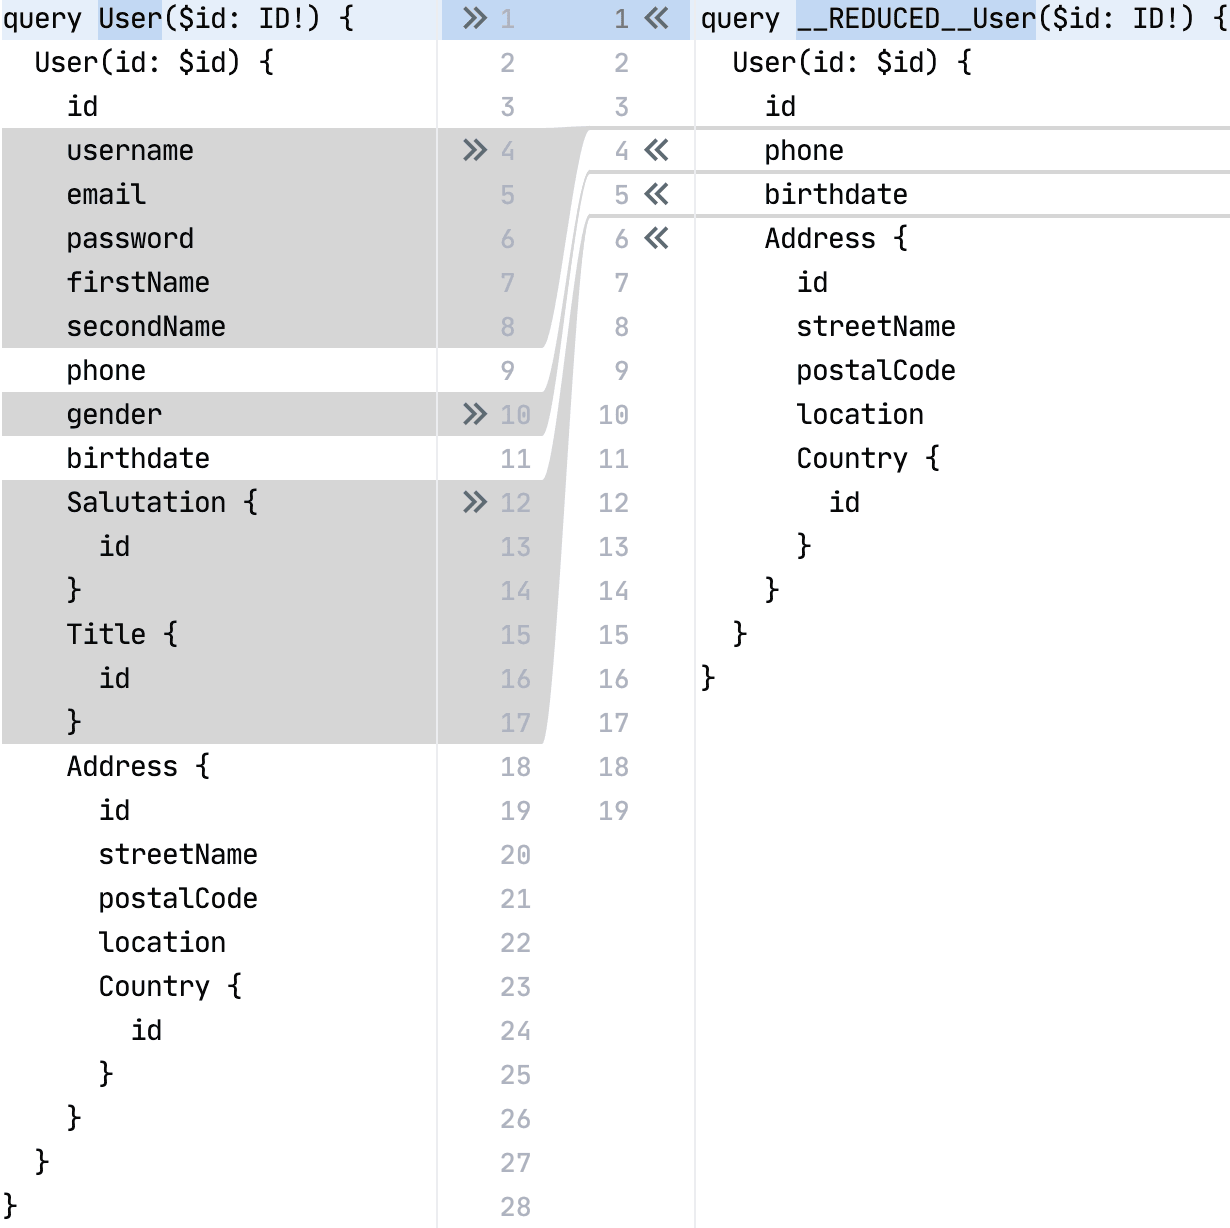
\includegraphics[width=0.65\linewidth]{images/reduction-graphql-examples/compare-user-reduced-user.png}
  \caption{A comparison of the original user- and reduced user-query.}\label{fig:applied-methods:comparison-user-reduced-user}
  \end{figure}
\fi


% \section{Persist the state of the cache}




\ifshowResultsChapter
  \chapter{Results}\label{chapter:results}

This chapter explains whether the micro-frontend architecture using GraphQL and a shared caching layer can improve performance over a separated cache. The micro-frontend architecture implements four \acp{SPA} and nine widgets. Most of the implementation was done using Angular, but one single widget was implemented in React. Using another framework should showcase whether another technology could access the shared caching layer. Furthermore, a \ac{BFF} service was developed using GraphQL which is explicitly tailored to the needs of the micro-frontends. The \ac{BFF} aggregates the data from the microservices and provides it to the micro-frontends. An overview of the prototypical architectures communicates with the GraphQL \ac{API} is shown in listing \ref{fig:results:micro-frontend-prototype}.

\ifshowImages
\begin{figure}[H]
  \centering
  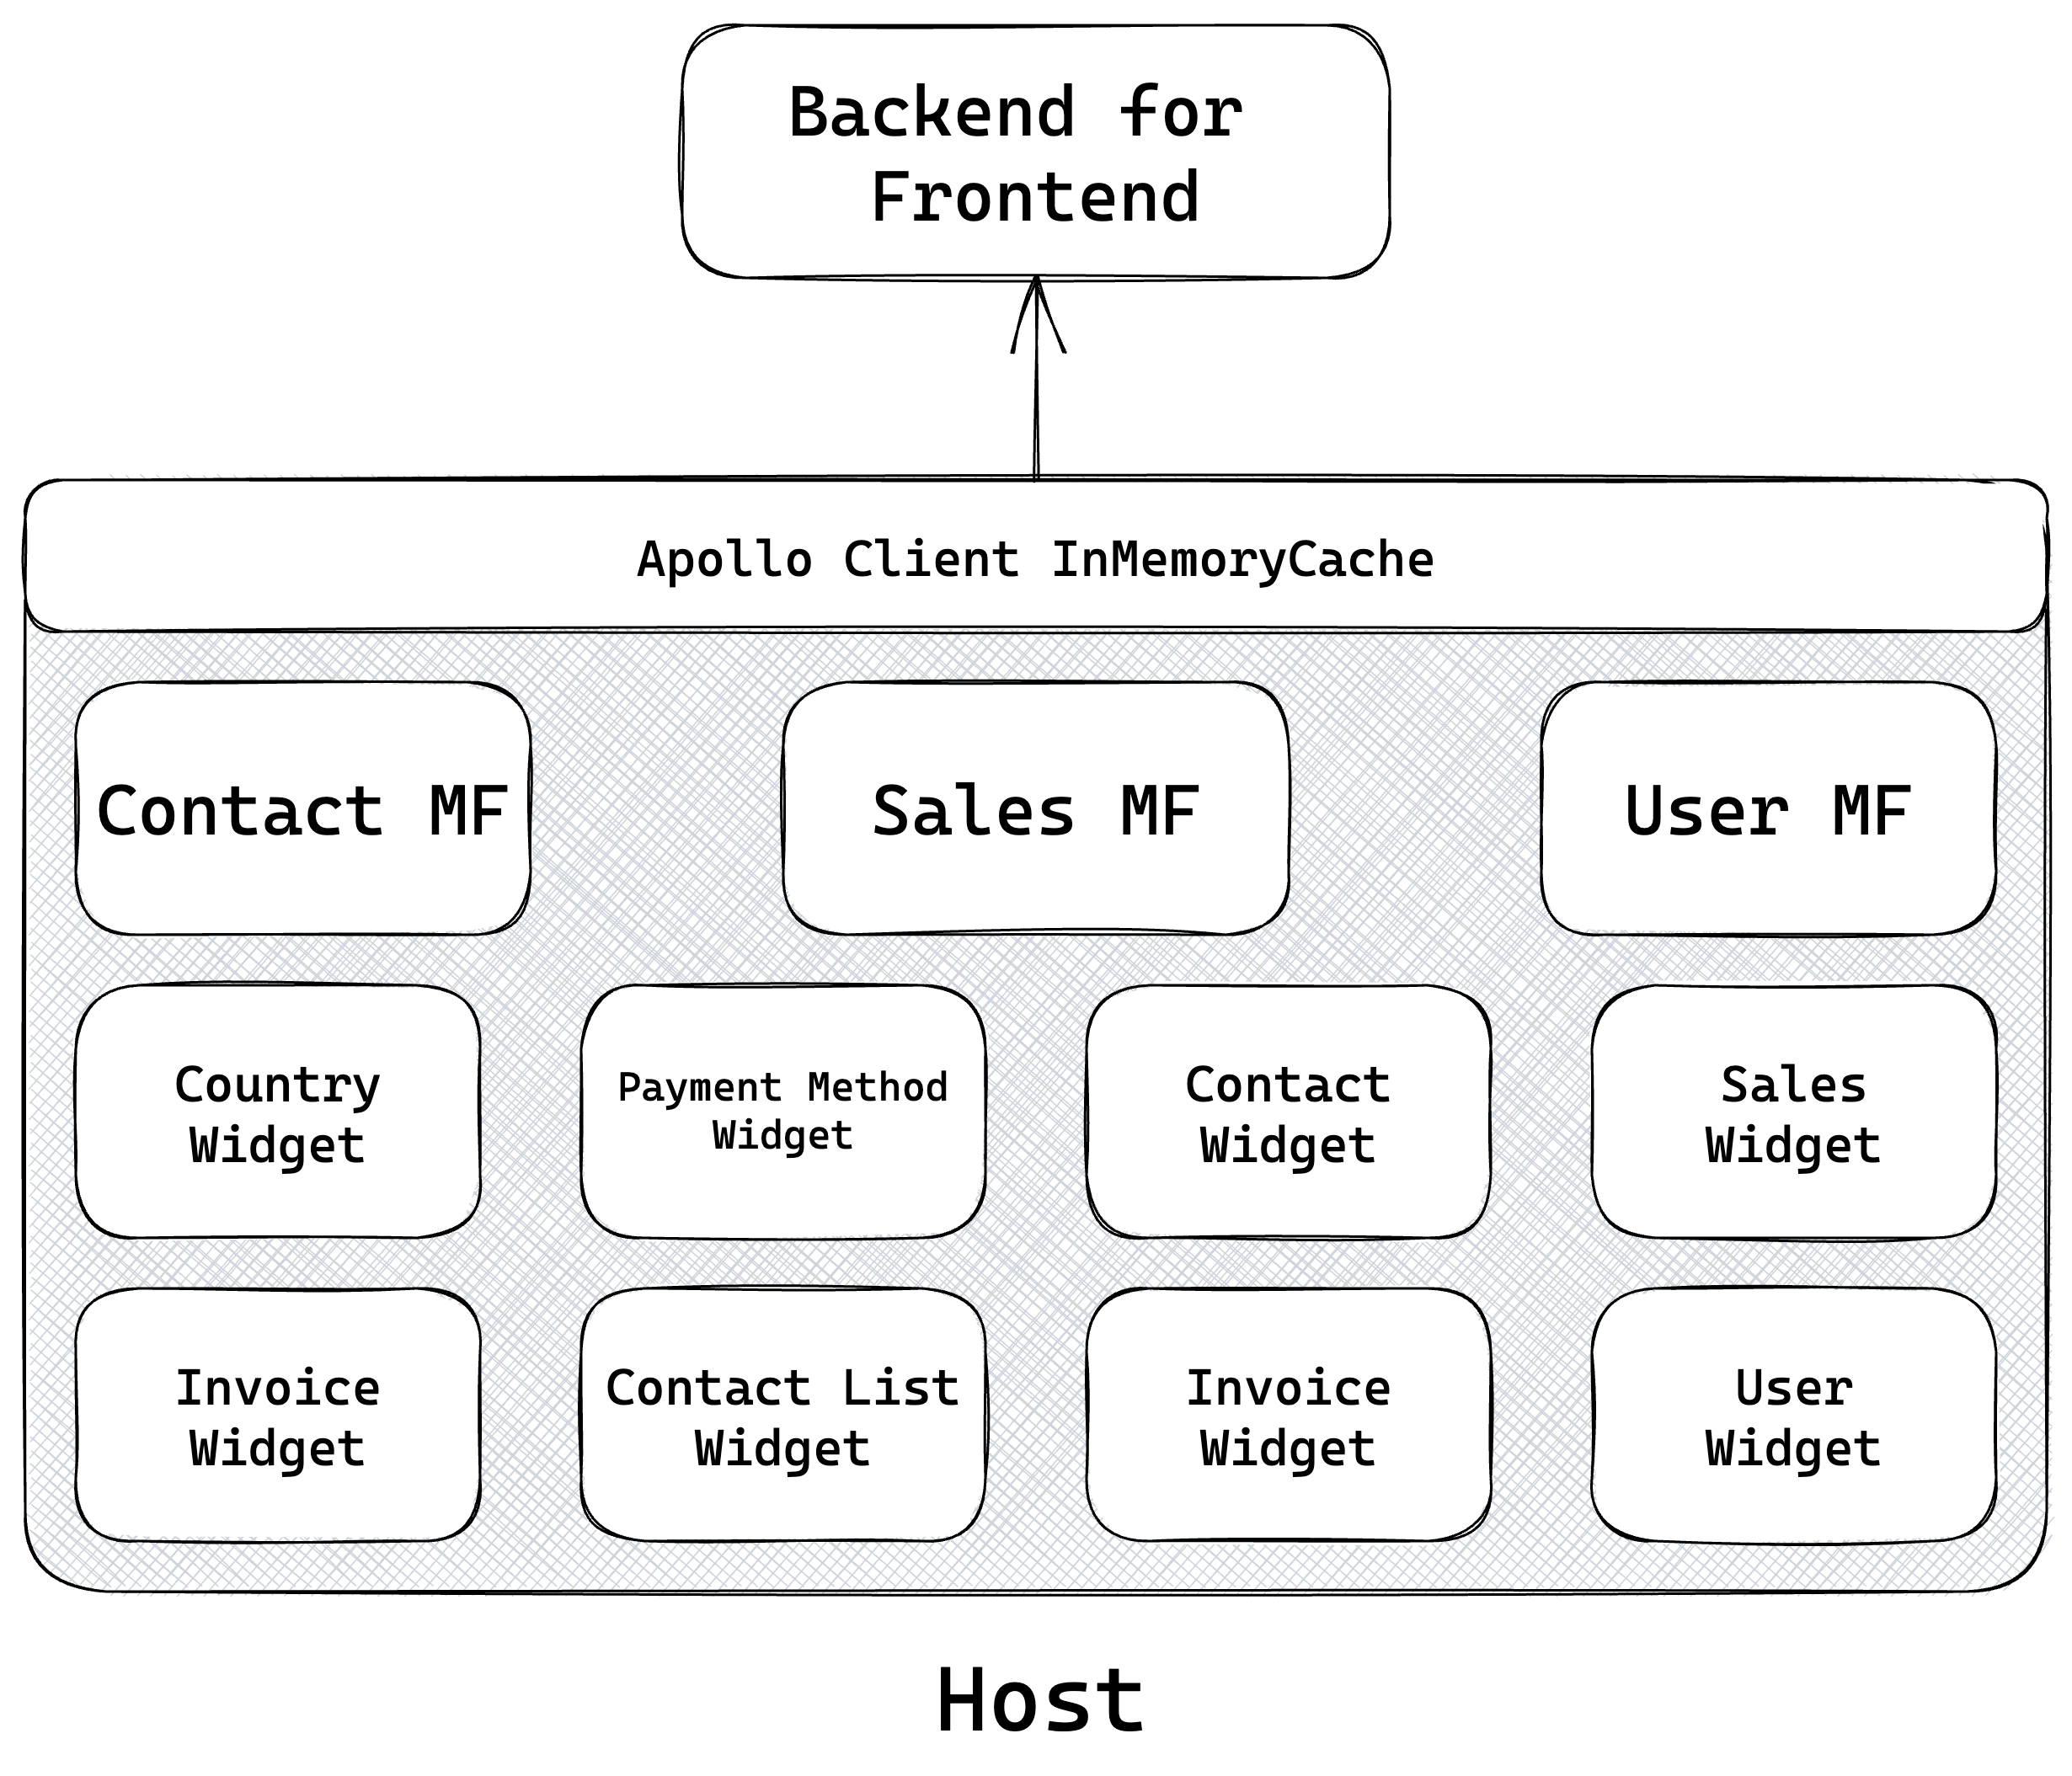
\includegraphics[width=0.8\linewidth]{images/results/micro-frontend-prototype.png}
  \caption{Architecture of the micro-frontend prototype.}\label{fig:results:micro-frontend-prototype}
\end{figure}
\fi

\section{Performance measurement}\label{section:results:performance-measurement}

This section explains how the micro-frontend architecture will be evaluated regarding the first hypothesis. Three distinct approaches were identified to measure the performance of the shared GraphQL caching layer. The architecture implements a switch allowing it to switch quickly between these three approaches.

\begin{enumerate}
  \item \textbf{Separate Cache and no reduced queries}: All remote modules use a separate cache, and no queries are reduced with the help of the cache.
  \item \textbf{Shared Cache and no reduced queries}: The remote modules share the same cache instance, and no queries are reduced with the help of the cache.
  \item \textbf{Shared Cache and reduced queries}: All remote modules share the same instance of the cache, and queries are reduced by using the functionality from apollo-augmented-hooks.
\end{enumerate}

\noindent Two exemplary paths through the application were planned to measure and compare the performance of these three approaches. These user journeys were intended to show how many network requests were made to the GraphQL \ac{API} and how much network traffic was generated during the process. A large amount of mock data was generated and used by the GraphQL \ac{API} to make the measurements as close as possible to real conditions. With this large amount of data, measuring the differences in response size is more expressive. Fetching smaller datasets makes only a difference when the application is used over a more extended period of time. The following sections detail the results of the user journeys through the application.

\section{Comparing the results of the first user journey}\label{section:results:comparison-first-journey}

This section takes the measurements from the previous section \ref{subsection:results:performance-measurement:evaluation} and compares the different approaches in terms of request sizes and response sizes, the number of requests, and the total records fetched.

\subsection{Comparing the first- and second-approach}\label{subsection:results:comparison-first-second-approach}

When comparing the first- with the second approach there is a significant difference in the number of network requests made to the GraphQL \ac{API} and the size of the requests and responses, as seen in table \ref{table:results:size-comparison-first-path-no-cache-no-reduction-cache-no-reduction}. The shared cache approach requires eleven fewer network requests than the separate cache approach. Since the queries are not reduced for this comparison, the additional network queries account for the overall difference in request- and response size. The 11 additional requests from the first approach send an additional 2.29 KB to the backend and return about an additional 2.34 MB from the backend. Therefore, 22\% of the total response size can be saved by using only one shared cache for all micro-frontends. Another interesting observation is that the shared cache approach retrieves 30191 fewer records than the naive approach, which is about 37\% of the total records returned.

\ifshowTables
\begin{table}[H]
  \begin{tabular}{|l|l|l|l|l|}
  \hline
    & \textbf{Request Size (B)} & \textbf{Response Size (B)} & \textbf{Requests} & \textbf{Records} \\
    \hline
    \textbf{No Reduction, Separate Cache} & 17462 & 10780656 & 47 & 81510 \\
    \hline
    \textbf{No Reduction, Shared Cache} & 15176 & 8437211 & 36 & 51319 \\
    \hline
    \hline
    \textbf{Diff} & \textbf{2286} & \textbf{2343445} & \textbf{11} & \textbf{30191} \\
    \hline
    \textbf{Reduction (\%)} & \textbf{13\%} & \textbf{22\%} & \textbf{23\%} & \textbf{37\%} \\
    \hline
  \end{tabular}
  \caption{First Journey: Comparing the requests and responses of the first- and second-approach.}\label{table:results:size-comparison-first-path-no-cache-no-reduction-cache-no-reduction}
\end{table}
\fi

\noindent The following enumeration shows which and how often GraphQL queries were dropped when using a shared caching layer between the micro front-ends compared to a separate cache:

\begin{itemize}
  \item allCountries: 2
  \item allSalutations: 2
  \item allTitles: 2
  \item allArticleUnits: 1
  \item allCurrencies: 1
  \item allVats: 1
  \item allSalesCountries: 1
  \item allInvoiceTypes: 1
\end{itemize}

\noindent The data of the requests that were omitted is usually used for filling selection controls inside detail views and has to be fetched over and over again in every micro-frontend. The first three queries are used for widgets on the dashboard, the contact application, and the user application. The last five queries are used for widgets on the dashboard and the sales application.

\subsection{Comparing the first- and third-approach}\label{subsection:results:comparison-first-third-approach}

Like in the previous comparison, there is the same difference in the number of network requests made to the GraphQL \ac{API}. The size of the responses and the requests have a massive difference, just like before. The results are shown in table \ref{table:results:size-comparison-first-path-no-cache-no-reduction-cache-reduction}. Just like before, there is a difference of 11 GraphQL queries that are sent to the GraphQL \ac{API}. However, due to the reduction in queries, the difference in the size of the queries and responses is greater than in section \ref{subsection:results:comparison-first-second-approach}. All queries of the first approach send 3.92 KB more and return about 2.41 MB more from the GraphQL \ac{API} compared to the third approach. A shared cache and query reduction can save about 22\% response sizes. As before, 37\% fewer records need to be fetched from the backend.

\ifshowTables
\begin{table}[H]
  \begin{tabular}{|l|l|l|l|l|}
  \hline
  & \textbf{Request Size (B)} & \textbf{Response Size (B)} & \textbf{Requests} & \textbf{Records}  \\
  \hline
  \textbf{No Reduction, Separate Cache} & 17462 & 10780656 & 47 & 81510 \\
  \hline
  \textbf{Reduction, Shared Cache} & 13533 & 8374763 & 36 & 51319 \\
  \hline
  \hline
  \textbf{Diff} & \textbf{3929} & \textbf{2405893} & \textbf{11} & \textbf{30191} \\
  \hline
  \textbf{Reduction (\%)} & \textbf{23\%} & \textbf{22\%} & \textbf{23\%} & \textbf{37\%} \\
  \hline
  \end{tabular}
  \caption{First Journey: Comparing the requests and responses of the first- and third-approach.}\label{table:results:size-comparison-first-path-no-cache-no-reduction-cache-reduction}
\end{table}
\fi

\subsection{Comparing the second- and third-approach}\label{subsection:results:comparison-second-third-approach}

Between the first- and the second approach, there is almost no difference in terms of request- and response size compared to the comparisons from section \ref{subsection:results:comparison-first-second-approach} and \ref{subsection:results:comparison-first-third-approach}, as seen in table \ref{table:results:size-comparison-first-path-no-cache-no-reduction-cache-reduction}. Both approaches have the same number of queries sent to the GraphQL \ac{API} since the cache is shared by all micro-frontends. Reducing queries does not lead to fewer network requests. The difference in request and response size between the two approaches comes solely from the use of query reduction. By using the third approach, the difference in request size is about 1.64 KB (11\%), which is not significant. The difference between the response sizes (62.45 KB) is almost zero in relation to the amount of data that was returned.

\ifshowTables
\begin{table}[H]
  \begin{tabular}{|l|l|l|l|l|}
  \hline
  & \textbf{Request Size (B)} & \textbf{Response Size (B)} & \textbf{Requests} & \textbf{Records} \\
  \hline
  \textbf{No Reduction, Shared Cache} & 15176 &  8437211 & 36 & 51319 \\
  \hline
  \textbf{Reduction, Shared Cache} &  13533 &  8374763 & 36 & 51319 \\
  \hline
  \hline
  \textbf{Diff} & \textbf{1643} & \textbf{62448} & \textbf{0} & \textbf{0} \\
  \hline
  \textbf{Reduction (\%)} & \textbf{11\%} & \textbf{0\%} & \textbf{-} & \textbf{-} \\
  \hline
  \end{tabular}
  \caption{First Journey: Comparing the requests and responses of the second- and third-approach.}\label{table:results:size-comparison-first-path-cache-no-reduction-cache-reduction}
\end{table}
\fi

\section{Compare the results of the second user journey}\label{section:results:comparison-second-journey}

This section compares the results for a second user journey through the prototype between the three approaches explained in Section \ref{section:results:performance-measurement}. The client's journey through the application is shown in Figure \ref{fig:results:evaluation-second-path}. The client has to perform 17 steps throughout the prototype, which involves running every available GraphQL query. In contrast to the first journey from Section \ref{section:results:comparison-first-journey}, the client uses an authenticated user to perform the test. The GraphQL \ac{API} query to retrieve the authenticated user is performed by every micro-frontend individually.

\ifshowImages
\begin{figure}[H]
  \centering
  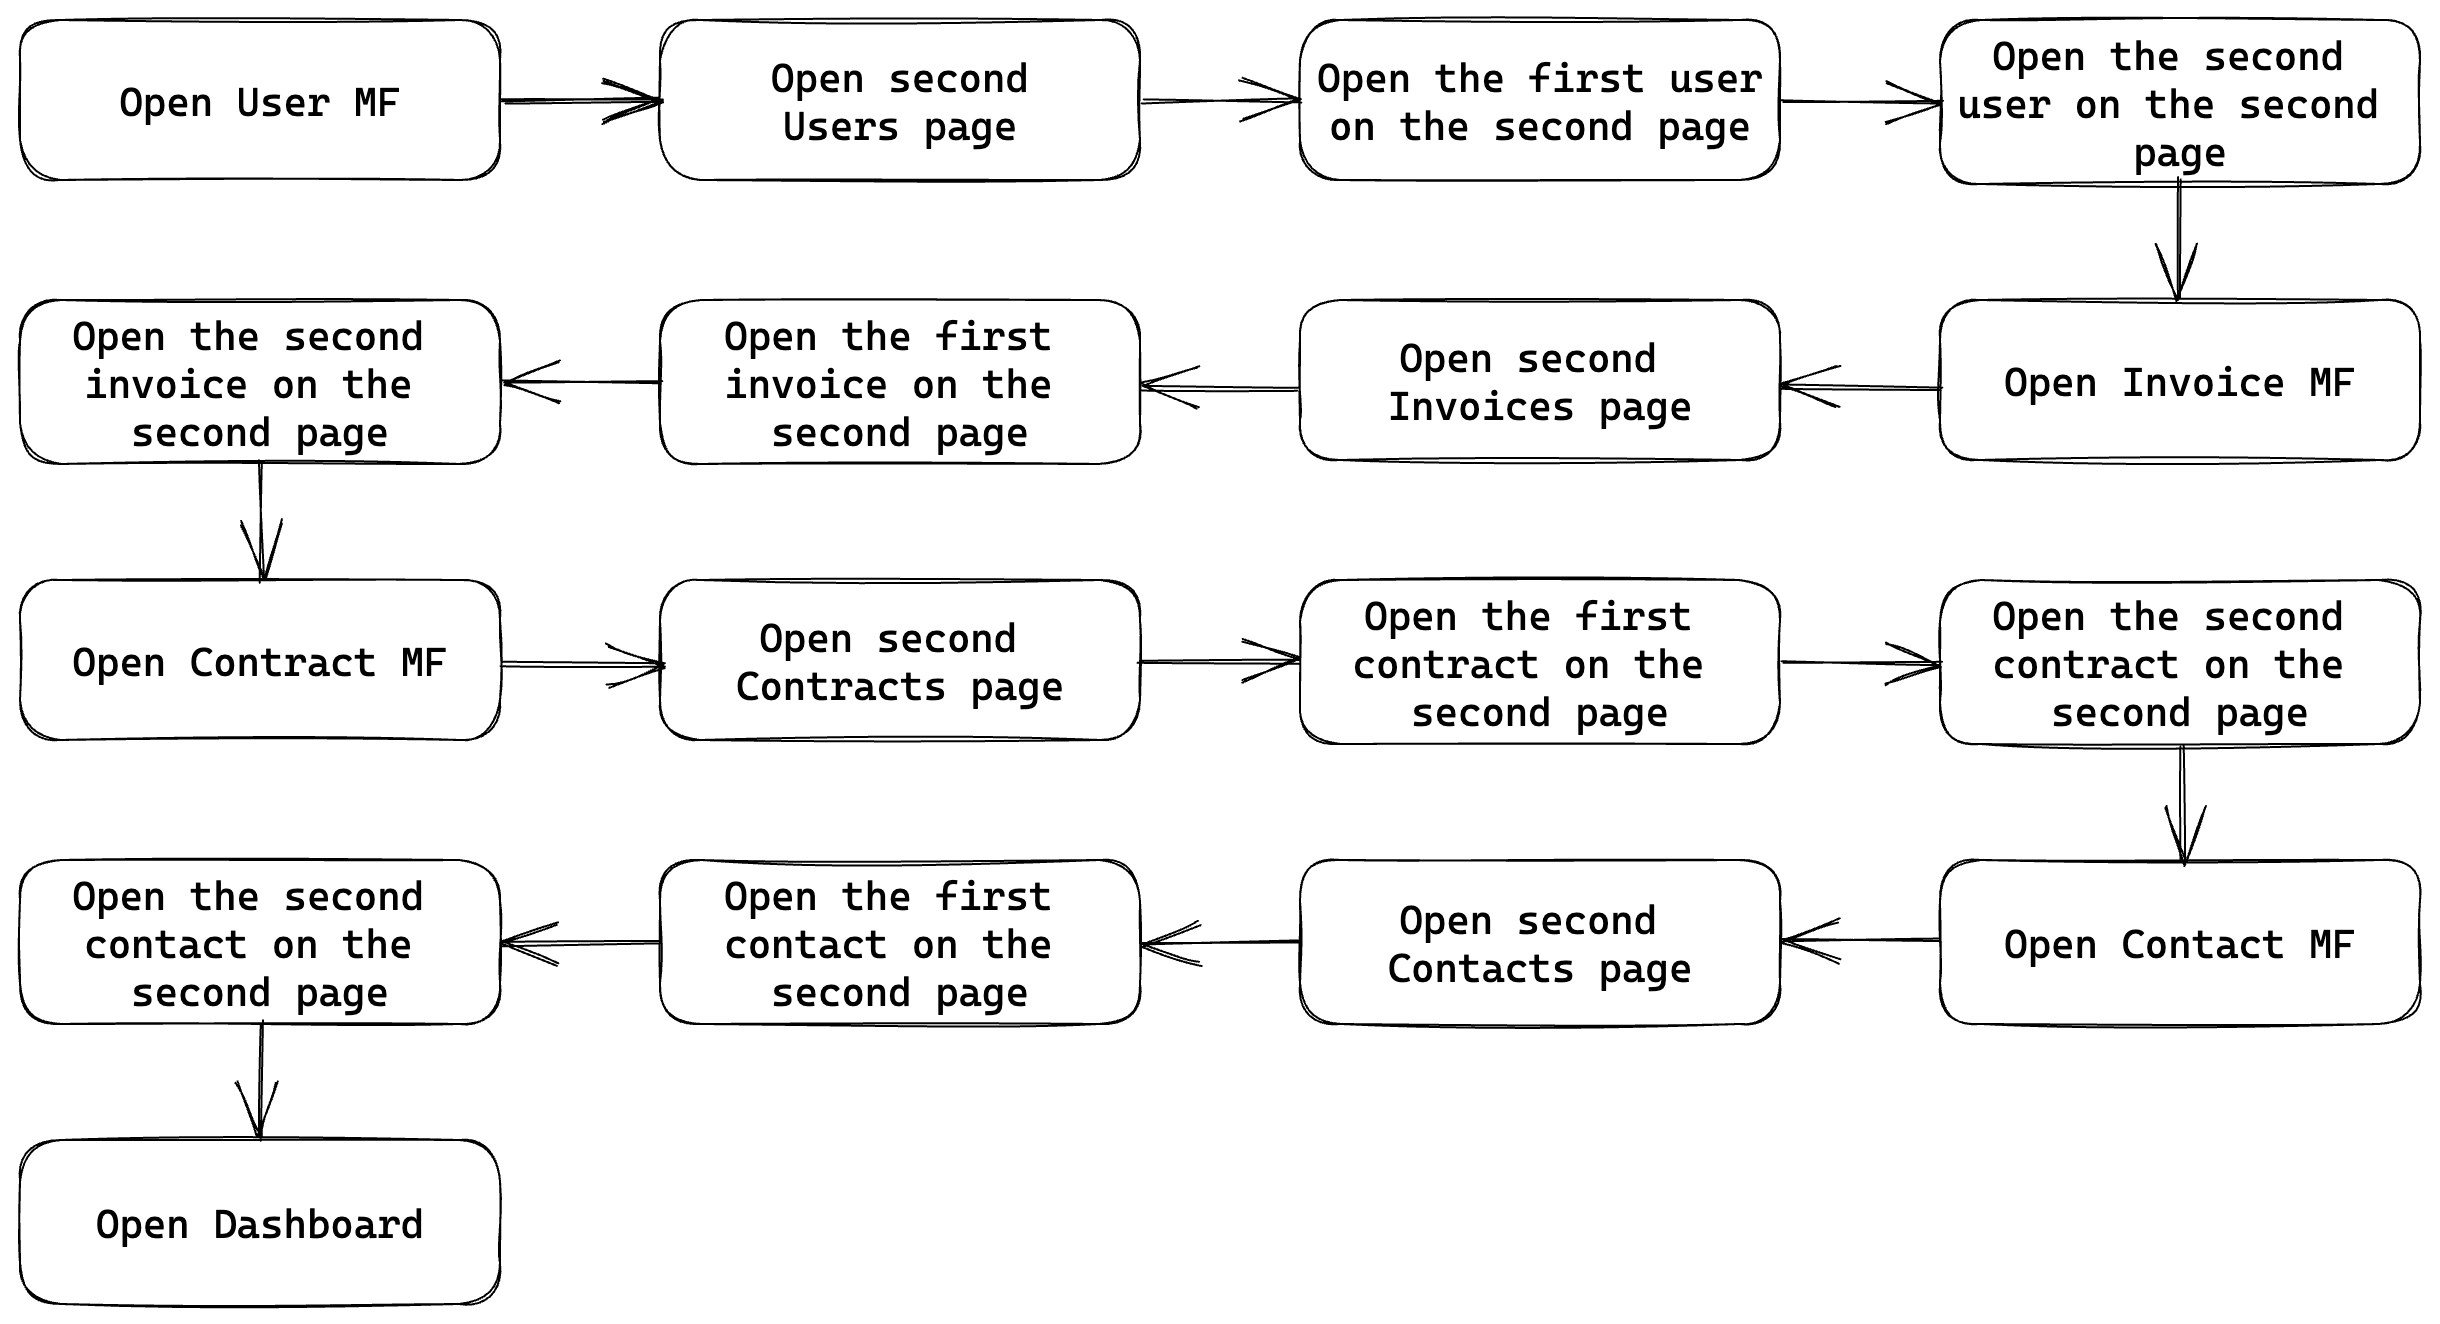
\includegraphics[width=1\linewidth]{images/results/evaluation-second-path.png}
  \caption{The second user journey through the application to measure the performance of the micro-frontend architecture.}\label{fig:results:evaluation-second-path}
\end{figure}
\fi

\noindent The following sections compare the three distinct approaches regarding request size, response size, number of requests, and the total number of records fetched, just as in the previous Section \ref{section:results:comparison-first-journey}.

\subsection{Compare the first- and second-approach}\label{subsection:results:comparison-second-path-first-second-approach}

Comparing the first approach with the second, there is a difference of 25 network requests to the GraphQL \ac{API} and the size of the requests and responses, as seen in Table \ref{table:results:size-comparison-second-path-cache-no-reduction-cache-reduction}. The second approach requires 25 fewer network requests than the first approach. Since the queries are not altered for this comparison, the additional network requests are responsible for the overall difference in request- and response size. The difference in request size is 26\%, which is about 6.07 KB, which is insignificant. Using a shared cache layer can save about 22\% of the total response size. Another interesting observation is that the shared cache approach retrieves 30401 fewer records than the naive approach, which is about 37\% of the total records returned.

\ifshowTables
\begin{table}[H]
  \begin{tabular}{|l|l|l|l|l|}
  \hline
  & \textbf{Req. size (B)} & \textbf{Resp. size (B)} & \textbf{Requests} & \textbf{Records} \\
  \hline
  \textbf{No Reduction, Separate Cache} & 22955 & 10713304 & 62 & 81325 \\
  \hline
  \textbf{No Reduction, Shared Cache} & 16884 & 8364416 & 37 & 50924 \\
  \hline
  \hline
  \textbf{Diff (B)} & \textbf{6071} & \textbf{2348888} & \textbf{25} & \textbf{30401} \\
  \hline
  \textbf{Reduction (\%)} & \textbf{26\%} & \textbf{22\%} & \textbf{40\%} & \textbf{37\%} \\
  \hline
  \end{tabular}
  \caption{Second Journey: Compare the requests and responses of the second- and third-approach.}\label{table:results:size-comparison-second-path-cache-no-reduction-cache-reduction}
\end{table}
\fi

\subsection{Compare the first- and third-approach}\label{subsection:results:comparison-second-path-second-third-approach}

As in the previous comparison, there are again 25 requests less made to the GraphQL \ac{API}. The size of the responses and the requests are similar to the previous section. The results are shown in Table \ref{table:results:size-comparison-second-path-no-cache-no-reduction-cache-reduction}. However, due to the reduction in queries, the difference in the size of queries and responses is more pronounced than in Section \ref{subsection:results:comparison-second-path-first-second-approach}. The difference in request size is 36\%, which accounts for 8.24 KB, which is insignificant. A shared caching layer and query reduction can save about 22\% of response size; as before, 37\% fewer records need to be fetched from the GraphQL \ac{API}.

\ifshowTables
\begin{table}[H]
  \begin{tabular}{|l|l|l|l|l|}
  \hline
  & \textbf{Req. size (B)} & \textbf{Resp. size (B)} & \textbf{Requests} & \textbf{Records} \\
  \hline
  \textbf{No Reduction, Separate Cache} & 22955 & 10713304 & 62 & 81325 \\
  \hline
  \textbf{Reduction, Shared Cache} & 14718 & 8361306 & 37 & 50924 \\
  \hline
  \hline
  \textbf{Diff (B)} & \textbf{8237} & \textbf{2351998} & \textbf{25} & \textbf{30401} \\
  \hline
  \textbf{Reduction (\%)} & \textbf{36\%} & \textbf{22\%} & \textbf{40\%} & \textbf{37\%} \\
  \hline
  \end{tabular}
  \caption{Second Journey: Compare the requests and responses of the first- and third-approach.}\label{table:results:size-comparison-second-path-no-cache-no-reduction-cache-reduction}
\end{table}
\fi

\subsection{Compare the second- and third-approach}\label{subsection:results:comparison-second-path-first-third-approach}

Between the second and third approaches, there is almost no difference regarding request size and response size. The results are displayed in Table \ref{table:results:size-comparison-second-path-no-cache-no-reduction-cache-no-reduction}. Both approaches have the same number of queries sent to the GraphQL \ac{API} and receive the same amount of records since all micro-frontends share the same cache instance. The difference in request and response size comes solely from using the query reduction mechanism. The difference in request size is 13\%, but they account for just 2.17 KB, which is insignificant. The difference between the response sizes (3.11 KB) is almost zero, like in the first user journey.

\ifshowTables
\begin{table}[H]
  \begin{tabular}{|l|l|l|l|l|}
  \hline
  & \textbf{Req. size (B)} & \textbf{Resp. size (B)} & \textbf{Requests} & \textbf{Records} \\
  \hline
  \textbf{No Reduction, Shared Cache} & 16884 & 8364416 & 37 & 50924 \\
  \hline
  \textbf{Reduction, Shared Cache} & 14718 & 8361306 & 37 & 50924 \\
  \hline
  \hline
  \textbf{Diff (B)} & \textbf{2166} & \textbf{3110} & \textbf{0} & \textbf{0} \\
  \hline
  \textbf{Reduction (\%)} & \textbf{13\%} & \textbf{0\%} & \textbf{-} & \textbf{-} \\
  \hline
  \end{tabular}
  \caption{Second Journey: Compare the requests and responses of the first- and second-approach.}\label{table:results:size-comparison-second-path-no-cache-no-reduction-cache-no-reduction}
\end{table}
\fi

\section{Compare original and reduced queries}

This section examines the differences in network request size and network response size between the reduced GraphQL queries and the unmodified original queries. The size difference between the original and reduced queries is calculated in percentages and bytes. Table \ref{table:code:comparison-user-reduction} shows the difference in network size for the user-detail query between the original and the reduced queries. The query fetches a user by its unique id. The network data was collected by fetching 10 different users from the GraphQL \ac{API} and looking at the request and response size. The requested fields of the user-detail query and which fields are removed fields with query reduction are explained in more detail in Section \ref{subsection:background:graphql:example-reduction}. The original query contains 16 fields, and 8 fields are removed from the query using the query reduction functionality. By removing 8 fields from the original GraphQL query, the size of the request to the GraphQL \ac{API} was reduced by about 30\% or 161 bytes. The difference in query sizes is always the same because the same 8 fields are removed from each user-detail query. When fetching 10 different users, a total of 1.61 KB of request size can be saved. The response size was reduced by 42\% on average. About 2.55 KB response size is saved when 10 different users are fetched from the GraphQL \ac{API} using query reduction. The response size difference varies slightly from user to user, because the content of the fields is different. The difference from the smallest to the largest user is only about 2\%.

\ifshowTables
\begin{table}[!htbp]
  \begin{tabular}{|l|l|l|l|l|}
  \hline
  \textbf{Query} & \textbf{Req. diff (\%)} & \textbf{Req. size diff (B)} & \textbf{Resp. diff (\%)} & \textbf{Resp. size diff (B)} \\
  \hline
  User A & 30\% & 161 & 42\% & 257 \\
  \hline
  User B & 30\% & 161 & 42\% & 257 \\
  \hline
  User C & 30\% & 161 & 41\% & 257 \\
  \hline
  User D & 30\% & 161 & 42\% & 244 \\
  \hline
  User E & 30\% & 161 & 43\% & 251 \\
  \hline
  User F & 30\% & 161 & 42\% & 271 \\
  \hline
  User G & 30\% & 161 & 42\% & 249 \\
  \hline
  User H & 30\% & 161 & 41\% & 263 \\
  \hline
  User I & 30\% & 161 & 41\% & 248 \\
  \hline
  User J & 30\% & 161 & 41\% & 252 \\
  \hline
  \hline
  \textbf{AVG} & \textbf{30\%} & - & \textbf{42\%} & -  \\
  \hline
  \hline
  \textbf{SUM} & - & \textbf{1610 (1.61 KB)} & - & \textbf{2549 (2.55 KB)} \\
  \hline
  \multicolumn{5}{l}{16 fields requested, 8 fields Removed, 8 remaining sent to the GraphQL \ac{API}}
  \end{tabular}
  \caption{A comparison of the user-detail query in request- and response-sizes.}\label{table:code:comparison-user-reduction}
\end{table}
\fi

% \bigskip

\noindent Table \ref{table:code:comparison-contract-reduction} shows the difference in network size for the contract-detail query between the original and reduced queries. The query fetches the detail data of a contract with its unique id. The network data was collected by fetching 10 different contracts. The original query contains 17 fields, where 10 fields were removed from the query using the query reduction functionality. Therefore, only 7 of the 17 fields remain within the query, which means that 58\% of the original fields were removed. The size of the requests to the GraphQL \ac{API} can be reduced by an average of 38\% or 207 bytes. Using the application and querying 10 detail views of a contract 2.07 KB of request size can be saved. The size GraphQL \ac{API} response can be reduced by about 58\% or 3.96 KB when fetching 10 different contracts. The response size savings vary slightly from contract to contract because the content of the fields is different. The difference from the smallest to the largest contract is only about 3\%.

\ifshowTables
\begin{table}[!htbp]
  \begin{tabular}{|l|l|l|l|l|}
  \hline
  \textbf{Query} & \textbf{Req. diff (\%)}  & \textbf{Req. size diff (B)} & \textbf{Resp. diff (\%)} & \textbf{Resp. size diff (B)}  \\
  \hline
  Contract A & 38\% & 207 & 58\% & 394 \\
  \hline
  Contract B & 38\% & 207 & 58\% & 378 \\
  \hline
  Contract C & 38\% & 207 & 59\% & 403 \\
  \hline
  Contract D & 38\% & 207 & 60\% & 408 \\
  \hline
  Contract E & 38\% & 207 & 60\% & 409 \\
  \hline
  Contract F & 38\% & 207 & 57\% & 370 \\
  \hline
  Contract G & 38\% & 207 & 58\% & 393 \\
  \hline
  Contract H & 38\% & 207 & 58\% & 407 \\
  \hline
  Contract I  & 38\% & 207 & 59\% & 400 \\
  \hline
  Contract J & 38\% & 207 & 58\% & 389 \\
  \hline
  \hline
  \textbf{AVG} & \textbf{38\%} & - & \textbf{58\%} & - \\
  \hline
  \hline
  \textbf{SUM} & - & \textbf{2070 (2.07 KB)} & - & \textbf{3951 (3.95 KB)} \\
  \hline
  \multicolumn{5}{l}{17 fields requested, 10 fields removed, 7 remaining sent to the GraphQL \ac{API}}
  \end{tabular}
  \caption{A comparison of the contract-detail query in request- and response-sizes.}\label{table:code:comparison-contract-reduction}
\end{table}
\fi

\fi

\ifshowDiscussionChapter
  \chapter{Discussion}\label{chapter:discussion}

This project report investigated whether GraphQL can bring performance improvement in micro-frontend architectures. The results of the evaluation of the prototype implementation of the micro-frontend architecture are discussed in this chapter. The results from Chapter \ref{chapter:results} are used to make a statement about the hypothesis from Chapter \ref{chapter:introduction}.

\section{Request Size}

Figure \ref{figure:discussion:request-size} displays the results already shown in the previous chapter as a bar chart. In terms of request-size the three approaches are not very far apart from each other. The reduction of queries only makes 1.64 KB difference, in contrast to only sharing the cache.

\ifshowImages
\begin{figure}[H]
\centering
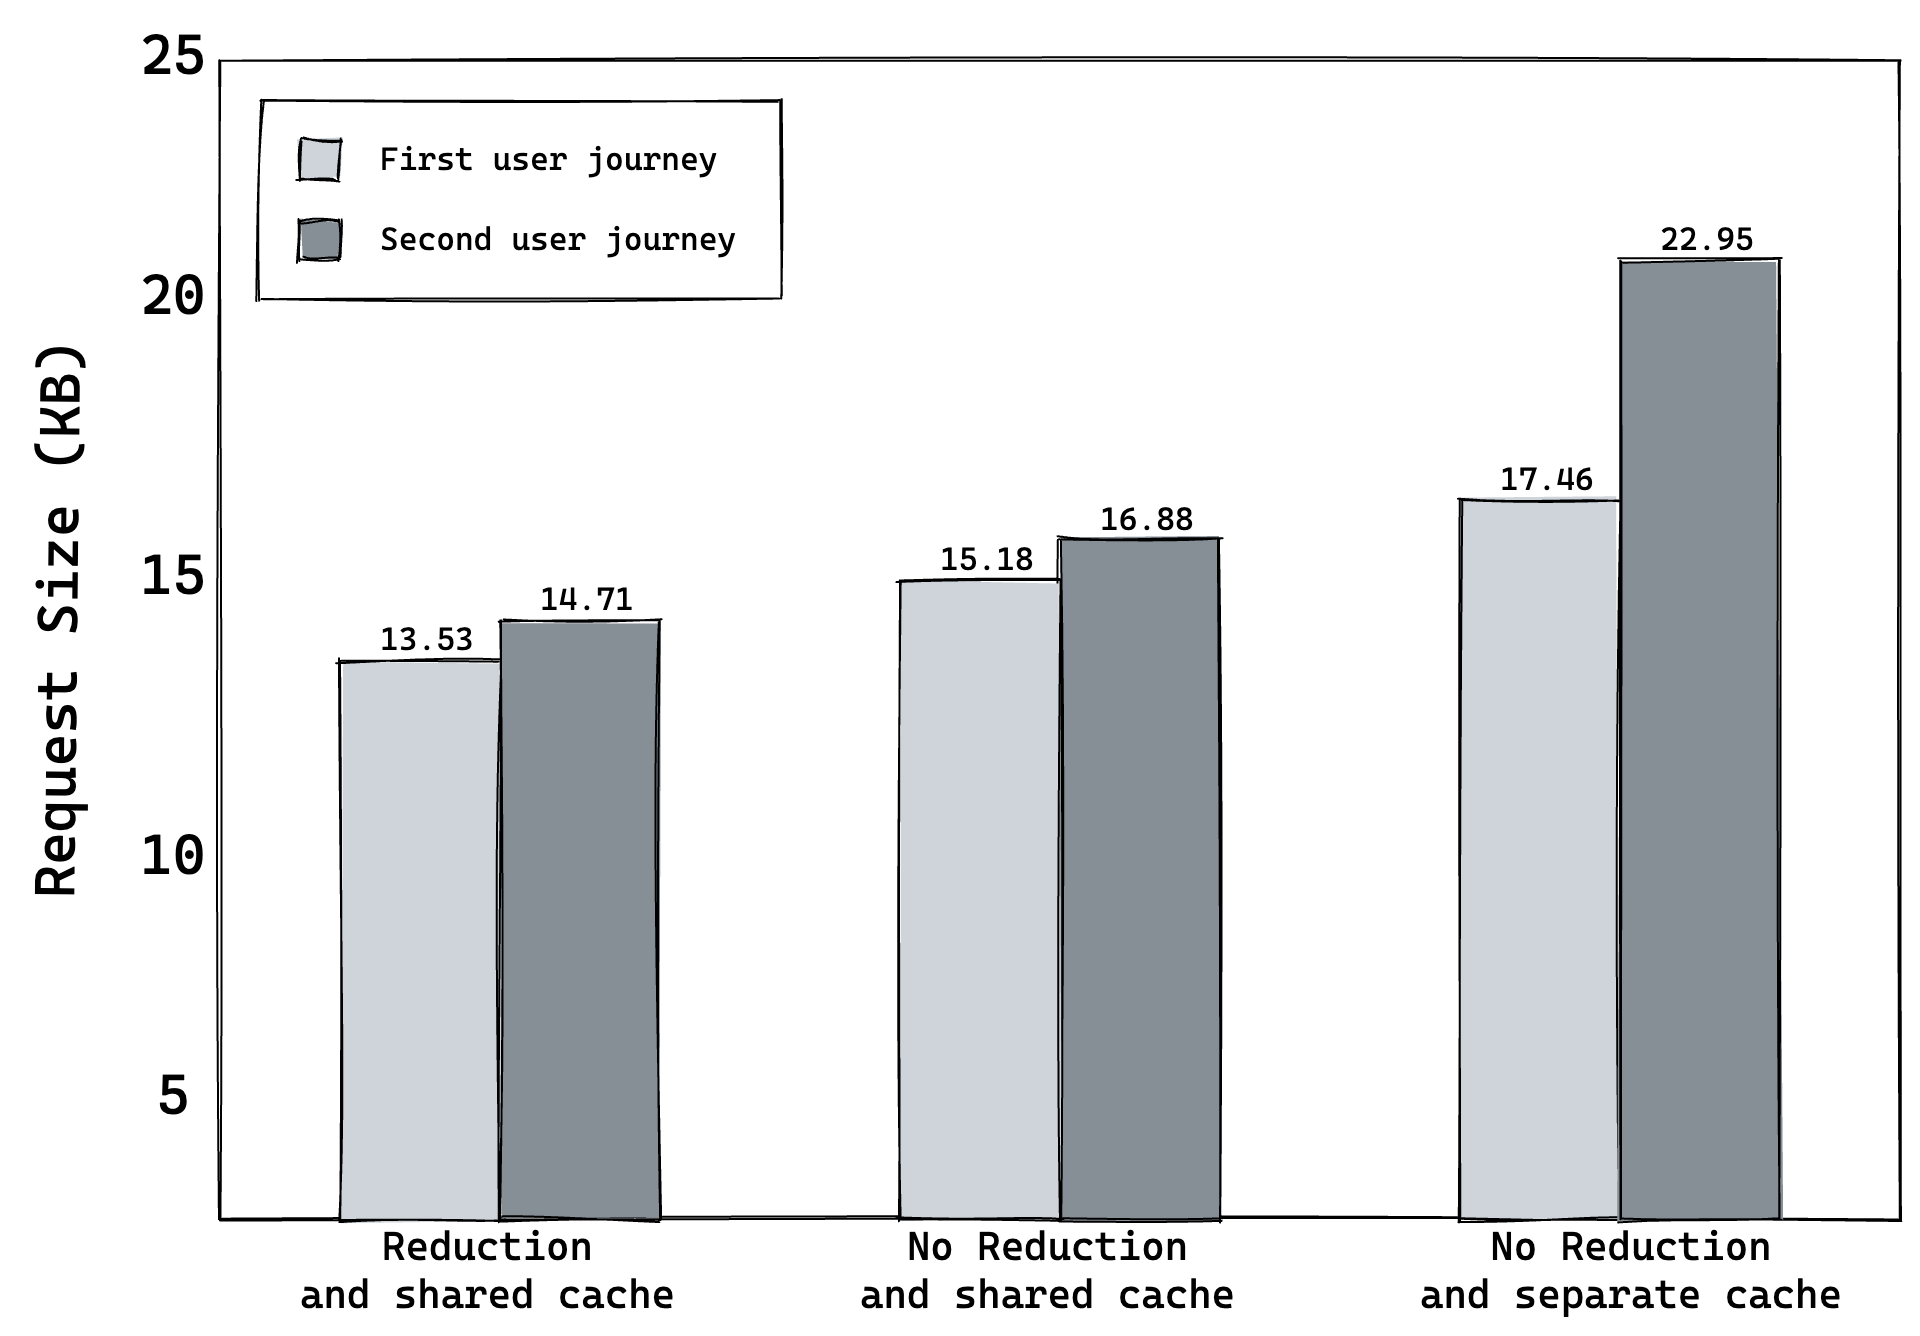
\includegraphics[width=0.8\linewidth]{images/discussion/request-size.png}
\caption{Request size comparison of the three approaches.}\label{figure:discussion:request-size}
\end{figure}
\fi

\section{Response Size}

Figure \ref{figure:discussion:response-size} displays the results already shown in the previous chapter as a bar chart. In contrast to the request-size, the response sizes are very far apart. When comparing the naive approach with the two improved approaches, there is a difference of about 2.40 MB. However, when comparing the two improved approaches, the difference is not very large. For the records that the application fetches, the reduction does not make such a big difference, in terms of responses.

\ifshowImages
\begin{figure}[H]
\centering
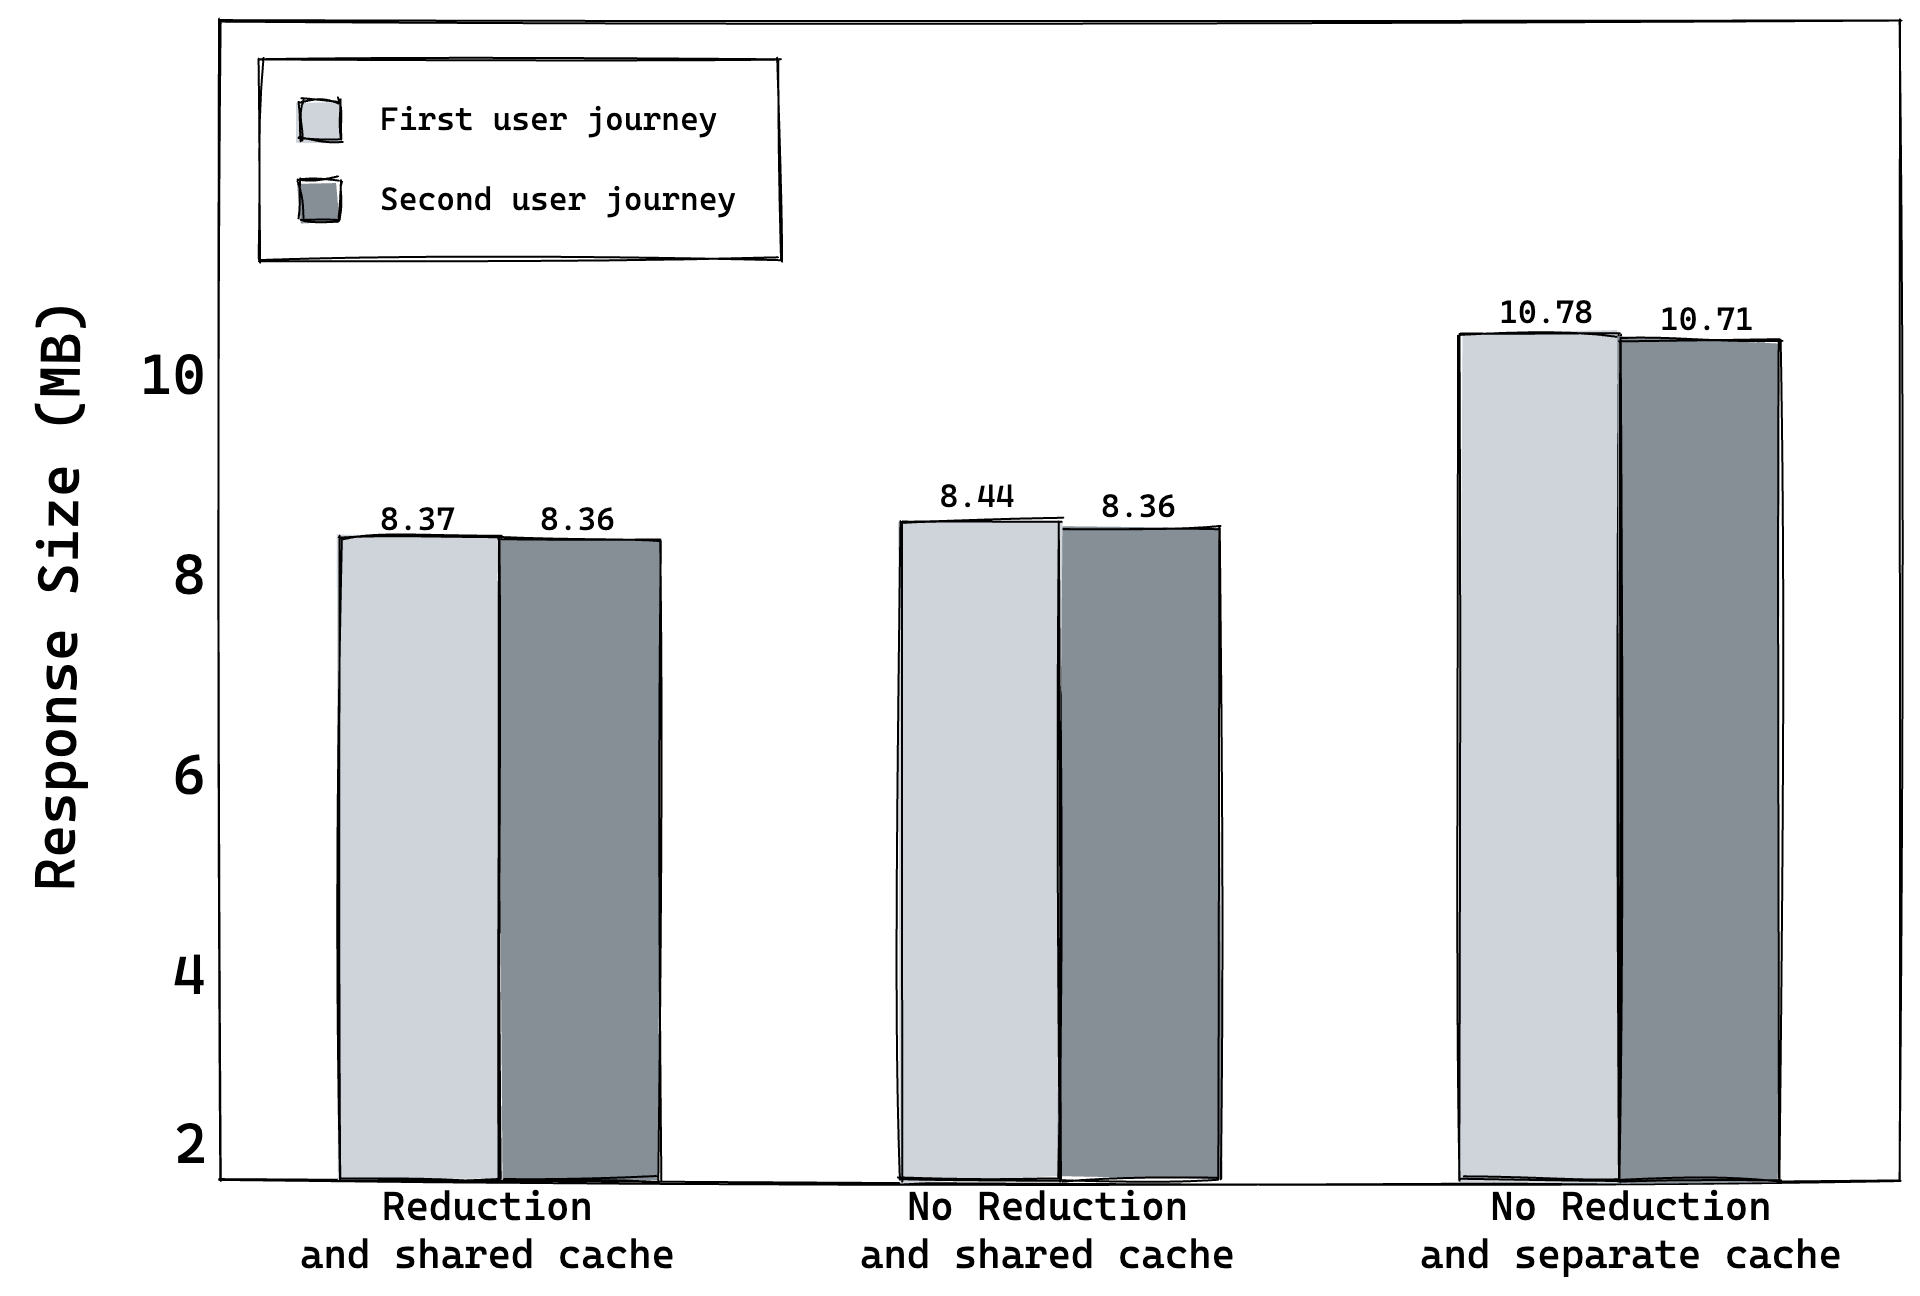
\includegraphics[width=0.8\linewidth]{images/discussion/response-size.png}
\caption{Response size comparison of the three approaches.}\label{figure:discussion:response-size}
\end{figure}
\fi

\fi

\ifshowConclusionChapter
  \chapter{Conclusion}\label{chapter:conclusion}

\noindent To validate the first hypothesis, which states that using GraphQL with a shared caching layer and a query reduction mechanism can prevent excessive retrievals and over-queries, a micro-frontend architecture with four \acp{SPA} and eight widgets was designed and implemented. An image showing the dashboard of the micro-frontend prototype is shown in Figure \ref{fig:conclusion:ui-dashboard}.

\ifshowImages
\begin{figure}[H]
  \centering
  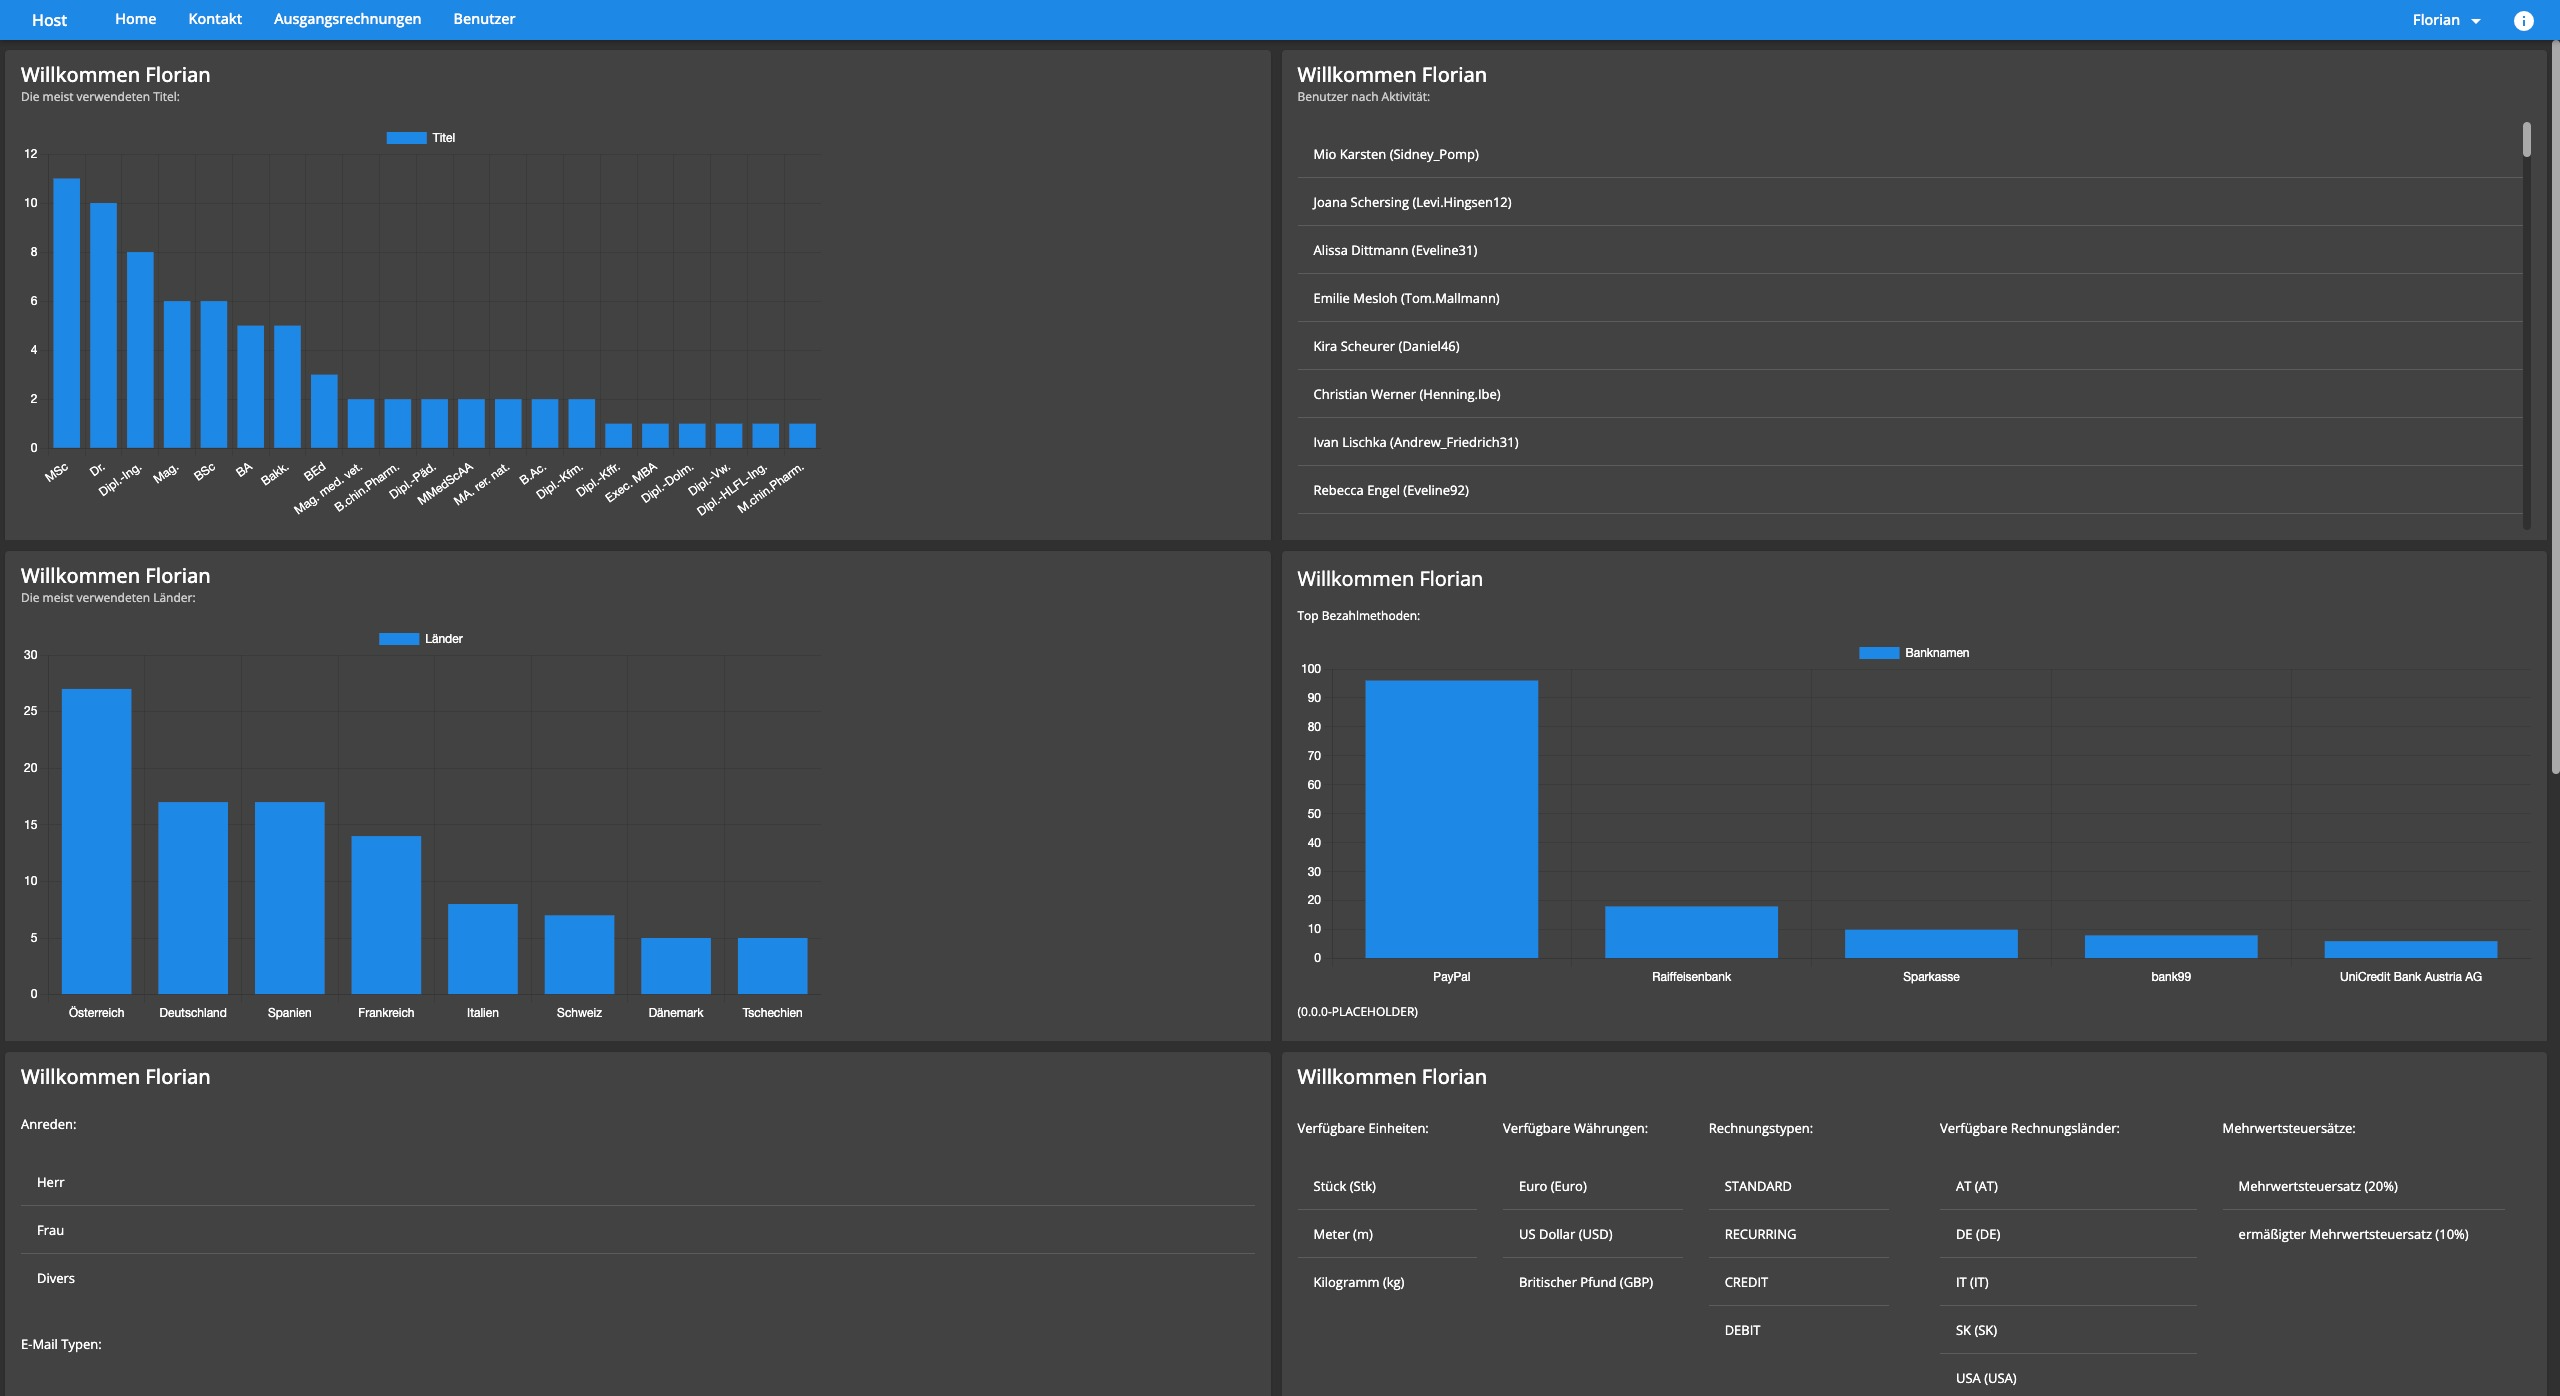
\includegraphics[width=1\linewidth]{images/prototype-screenshots/ui-dashboard.png}
  \caption{The dashboard of the micro-frontend prototype.}\label{fig:conclusion:ui-dashboard}
\end{figure}
\fi

\noindent Before the implementation began, the old legacy system was analyzed to identify potential bounded contexts that could be extracted into separate micro-frontends. The prototype was implemented using mainly Angular and React for a single widget. The micro-frontends were integrated using client-side integration using Webpack's Module Federation. A \ac{BFF} service in the form of a GraphQL \ac{API} was implemented using Apollo Server. This service provides a gateway to the microservice \acp{API} that run inside the company's cluster. The \ac{BFF} takes care of fetching and aggregating the data from multiple microservice. The data from the microservices is later used to answer GraphQL queries. The GraphQL \ac{API} was querying and mutating mocked datasets during development because the microservice cluster was not fully operational. The micro-frontend prototype will be integrated into the company's infrastructure sometime in the future and it will replace the legacy \ac{ERP} system. Therefore, the GraphQL schema and queries will be used later in production, making the evaluations' results very expressive.

\bigskip

\noindent The first step was to implement a communication strategy where the application shell could pass information to the micro-frontends. The shared caching layer was implemented with the help of Angular's \ac{DI}, which laid the groundwork for the communication strategy. To further improve the performance of the shared caching layer, a mechanism was implemented to provide the micro-frontend with the possibility to remove fields from GraphQL queries that are already stored inside the \texttt{InMemoryCache}. This behavior is not natively implemented in Apollo Client, but the apollo-augmented-hooks library offers exactly that functionality. However, the library is outdated and lacked support for \ac{JS} frameworks other than React. Therefore, the library was forked, and the functionality was made technology agnostic. Several new features were added to further leverage the \texttt{InMemoryCache} and remove unnecessary fields from a query.

\bigskip

\noindent Three different configurations for the micro-frontends were identified to compare whether the shared caching layer and the reduction of queries improve performance. The first approach is a naive approach where every micro-frontend has a separate cache and the queries are sent unaltered to the GraphQL \ac{API}. The second approach uses only the shared caching layer. The third approach uses the shared caching layer and reduces GraphQL queries by removing fields, that are already in the cache. Comparing the results of the measurements came with surprising results. The shared caching layer brought immense performance gains by significantly reducing the number of network requests and the overall size of network responses by several megabytes. However, reducing queries with the help of apollo-augmented-hooks functionality did not yield the expected results. In contrast to the immense savings from the shared caching layer, reducing queries does not make a significant difference when comparing the request and response sizes. Maintaining the additional functionality to reduce queries with the help of the cache brings additional complexity to the prototype. Each new release of Apollo Client's \texttt{InMemoryCache} could break the implementation, as the library directly depends on the cache's inner workings. When Apollo Client changes the public \ac{API}, it can disrupt the query reduction workflow. Another difficulty in using the query reduction mechanism is outdated and inconsistent data. If only fields that are not yet in the cache are retrieved, the objects in the cache may differ from their server counterparts. Especially with rapidly changing data, stale and new data can be mixed in the same cache object. The Apollo Client provides fetch policies to handle rapidly changing data, but they make the use of query reduction unnecessary. The user journeys of the built prototype do not leverage the potential of query reduction. The prototype mainly consists of a list view and a detail view. In this scenario, the potential of query reduction is not exploited because only a few fields are omitted from the queries. The list view usually shows only a handful of fields that could be removed from a query. These fields mostly contain a tiny fraction of response size. Most savings in response size can be made by omitting queries, which is already done by the shared caching layer

\bigskip

\noindent Based on the discussion points, hypothesis I is partially confirmed. The number of requests and network traffic can be drastically reduced with the help of a shared caching layer. This approach is a simple and relatively easy-to-implement solution that delivers huge performance improvements. Nevertheless, using a mechanism to remove existing fields from a query does not bring the desired performance improvements in the context of this prototype. 

\bigskip

\noindent Query reduction does not work well with the way data is retrieved within the prototype, as explained previously. Nevertheless, other applications might greatly benefit from such functionality. A major drawback of Apollo Client's \texttt{InMemoryCache} is that if the same query is retrieved twice and the second query contains a field that was not already in the first query, the query is always executed against the GraphQL \ac{API}. The other way around works well. If a query contains only fields or a subset of the fields that are already in the cache, the data for the query will be served only from the cache. Another disadvantage is that caching works only at the query level. The prototype mostly fetches part of the data in a list view and the complete data in a detail view. With the default behavior of Apollo Client, the query is always executed against the cache because the query name is different. The \texttt{InMemoryCache} does not know that parts of the detail data are already in the cache because another query retrieved them. The only solution to this problem is to define a cache redirect for each type, which is quite cumbersome.

\bigskip

\noindent To validate the second hypothesis, which states that the caching strategy implemented in this thesis can be used in various contexts and has enough flexibility to be technology agnostic, a micro-frontend was written in React and integrated into the application shell. Module Federation is a great tool to make encapsulated functionality and business logic available to be consumed by other applications. This allows micro-frontend architectures to be built independently of the framework used. To integrate the React application into the shared caching layer, an adapter Angular component was implemented. This component is responsible for initializing the React component and passing the information from the application shell to the React component. The base functionality of reducing queries was extracted into a library and an adapter for Angular and React was written. The concept of sharing a caching layer is technology agnostic and can be used independently of the framework. The only requirement is that the framework supports Apollo Client. Therefore, the second hypothesis is confirmed in the context of this thesis.

\fi

\ifshowFutureWorkChapter
  \chapter{Future work}\label{chapter:future-work}

This master thesis was primarily focused on implementing a prototypical micro-frontend architecture to replace AGnet's internal \ac{ERP} system sometime in the future. The work examined whether using GraphQL with Apollo Client can bring performance improvements inside a micro-frontend architecture. The improvements with GraphQL were implemented with two methods. First, a caching layer was shared across all micro-frontends. Second, the GraphQL Client layer should remove fields from queries that are already stored within the cache. Using a single cache instance for all micro-frontends has led to significant improvements regarding request size and response size. The second method of improving performance by reducing the fields of a query was auspicious, but it did not produce significant improvements in the prototype scenario. The screen design and structure of the prototype follow the approach of a list view, showing a table with some fields. In addition, a detail view for each table row view mainly loads all the fields in the object; however, the table view does not prefetch and cache enough fields to make a difference in query and response size. However, other applications with a different design could benefit from reducing queries with existing data. The following section explains a theoretical example of an application that could benefit from reducing queries.

\subsubsection{Example of an e-commerce platform benefiting from query reduction and a shared cache layer}

This section describes a fictional application that could improve significantly using query reduction and a shared caching layer. The application is an e-commerce platform, which has the same architecture as the micro-frontend prototype. The e-commerce application contains multiple micro-frontends, each responsible for a different part of the shopping experience. The micro-frontends for an e-commerce application could include multiple widgets on the landing page, product browsing, product detail, shopping cart, checkout process, and order tracking. A possible journey through an e-commerce application is shown in Figure \ref{fig:future-work:flow-chart}.

\ifshowImages
\begin{figure}[H]
  \centering
  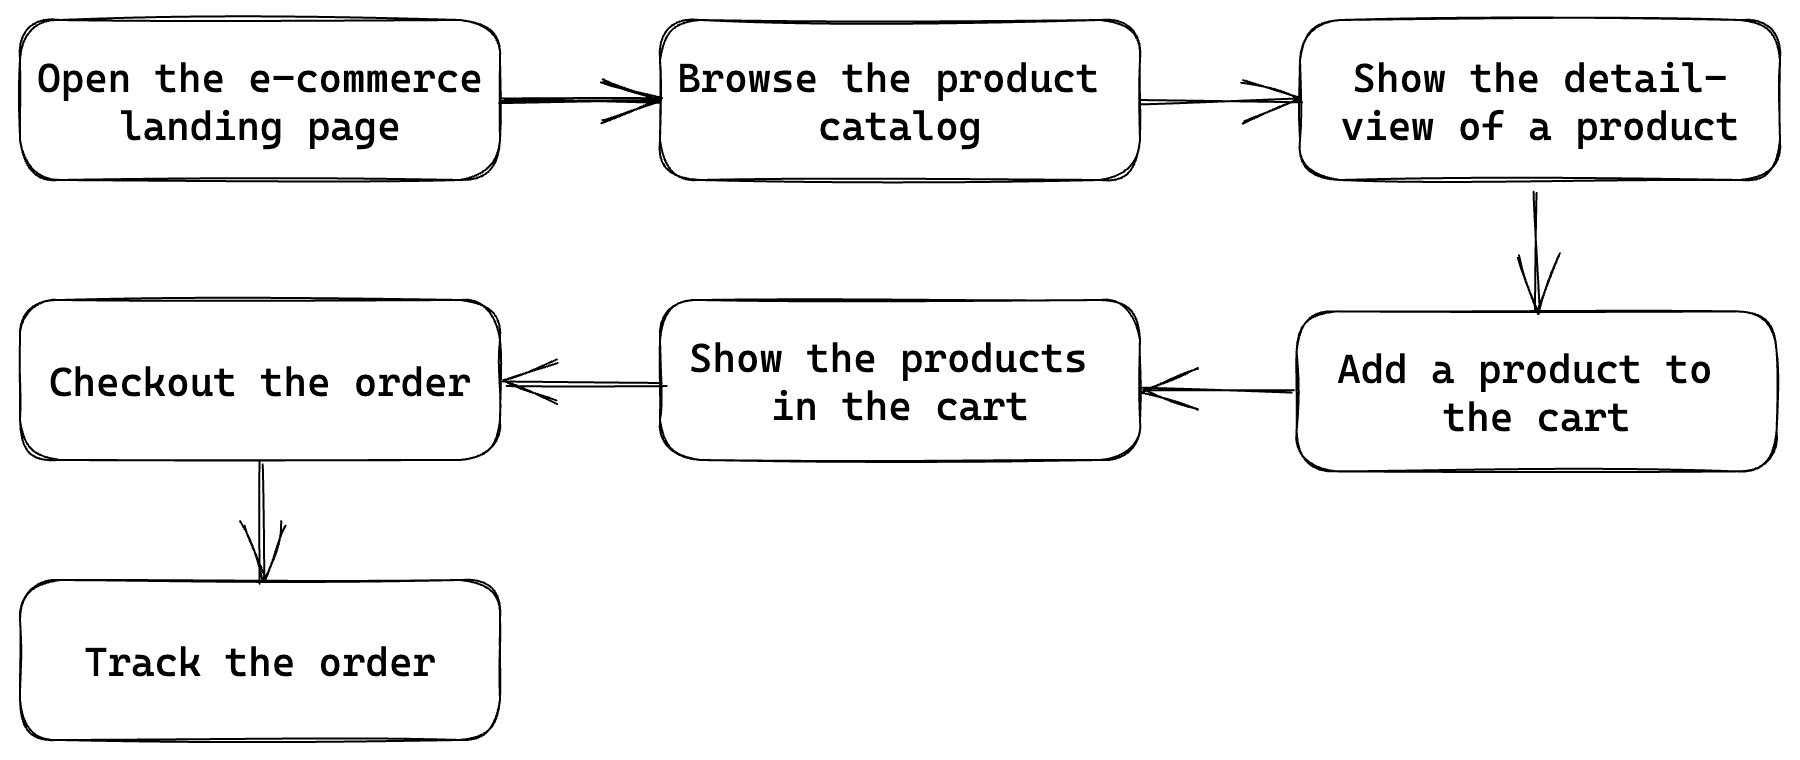
\includegraphics[width=0.8\linewidth]{images/future-work/flow-chart-e-commerce.png}
  \caption{A possible user journey through an e-commerce application.}\label{fig:future-work:flow-chart}
\end{figure}
\fi

\noindent The user first opens the landing page of the e-commerce platform. There he sees a list of recommended products and a list of product categories. The images and some information about the suggested products are loaded and stored in the cache. The user clicks on a recommended category and is redirected to the product browsing micro-frontend. The product browsing page displays a list of products in the selected category. The first products shown in the category are the same as on the landing page. Therefore, some data, including the product name, user rating, price, and image, can be reused from the cache. If the user scrolls down, the missing products are loaded from the server, rendered to the screen, and stored in the cache. Once the user finds a product they like, they can view the detail view. The detail view shows the product name, images, price, description, user rating, and reviews of other users. Much of the more important data, such as the product images displayed on the page, can be reused from the cache, allowing the page to render faster. Once the user has found a product he wants to order, he can add it to the shopping cart. When the user is ready to purchase the items in his shopping cart, he proceeds to the checkout. At the checkout, the user's address, the selected products and the total price are displayed. The information about the products can be completely reused from the cache. The information about the user's address can be reused from the cache. They enter their shipping and billing information, choose a payment method, and verify their order information. After submitting the order, the user receives a confirmation page with the order number, the ordered products and the expected delivery date. The user can track the status of his order and the progress of delivery. This information can also be fully reused from the cache if it is the same session.

\bigskip

\noindent This type of application benefits greatly from the shared caching layer and the mechanism for removing fields from a query that are already in the cache. The products are the main citizens of the e-commerce application. The shared caching layer is as important as it is in the micro-frontend prototype and allows most of the information to be reused. The user sees the same products on the landing page, product overview page, product detail page, shopping cart, checkout process, and order summary. So the product data is cached and can be used and extended on each page, which also benefits the subsequent pages.

\subsubsection{Further prototype development}

The current focus is on the further development of the micro-frontend prototype. The prototypical implementation carried out in this master thesis has only implemented a small subset of the functional requirements of the overall system. However, the basic structure that all micro-frontends must follow was defined and easily accessible. The process of creating, integrating, and configuring a new micro-frontend is also clearly defined and follows a standardized principle. The steps to create, configure, and add a new micro-frontend to the architecture could be automated in the future using Angular's Schematics\footnote{\url{https://angular.io/guide/schematics}}.

\fi


%
% Hier beginnen die Verzeichnisse.
%
\clearpage
\printbibliography
\clearpage

% Das Abbildungsverzeichnis
\listoffigures
\clearpage

% Das Tabellenverzeichnis
\listoftables
\clearpage

% Das Quellcodeverzeichnis
\listoflistings
\clearpage

\phantomsection
\addcontentsline{toc}{chapter}{\listacroname}

\chapter*{\listacroname}
\begin{acronym}[XXXXX]
    \acro{HTTP}{Hypertext Transfer Protocol}
    \acro{URL}{Uniform Resource Locator}
    \acro{API}{Application Programming Interface}
    \acro{SPA}{Single-Page-Application}
    \acro{BFF}{Backend For Frontend}
    \acro{REST}{Representational State Transfer}
    \acro{IP}{Internet-Procotol}
    \acro{HTML}{Hypertext Markup Language}
    \acro{IDE}{Integrated development environment}
    \acro{JSON}{JavaScript Object Notation}
    \acro{SQL}{Structured Query Language}
    \acro{GRPC}{gRPC Remote Procedure Calls}
    \acro{JS}{JavaScript}
    \acro{TS}{TypeScript}
    \acro{DI}{Dependency Injection}
    \acro{UI}{User Interface}
    \acro{ID}{Identifier}
    \acro{UML}{Unified Modeling Language}
\end{acronym}

%
% Hier beginnt der Anhang.
%
\clearpage
\appendix
\chapter{Anhang A}
\clearpage
\chapter{Anhang B}
\end{document}
